\documentclass[12pt,]{article}
\usepackage{lmodern}
\usepackage{amssymb,amsmath}
\usepackage{ifxetex,ifluatex}
\usepackage{fixltx2e} % provides \textsubscript
\ifnum 0\ifxetex 1\fi\ifluatex 1\fi=0 % if pdftex
  \usepackage[T1]{fontenc}
  \usepackage[utf8]{inputenc}
\else % if luatex or xelatex
  \ifxetex
    \usepackage{mathspec}
  \else
    \usepackage{fontspec}
  \fi
  \defaultfontfeatures{Ligatures=TeX,Scale=MatchLowercase}
\fi
% use upquote if available, for straight quotes in verbatim environments
\IfFileExists{upquote.sty}{\usepackage{upquote}}{}
% use microtype if available
\IfFileExists{microtype.sty}{%
\usepackage{microtype}
\UseMicrotypeSet[protrusion]{basicmath} % disable protrusion for tt fonts
}{}
\usepackage[margin=2.5cm]{geometry}
\usepackage{hyperref}
\hypersetup{unicode=true,
            pdftitle={Project 1: regression 1 (fishermen - do not use the variable MeHg)},
            pdfauthor={Urvan Christen, Amandine Goffeney, Joseph Vermeil, Lucile Vigué},
            pdfborder={0 0 0},
            breaklinks=true}
\urlstyle{same}  % don't use monospace font for urls
\usepackage{color}
\usepackage{fancyvrb}
\newcommand{\VerbBar}{|}
\newcommand{\VERB}{\Verb[commandchars=\\\{\}]}
\DefineVerbatimEnvironment{Highlighting}{Verbatim}{commandchars=\\\{\}}
% Add ',fontsize=\small' for more characters per line
\usepackage{framed}
\definecolor{shadecolor}{RGB}{248,248,248}
\newenvironment{Shaded}{\begin{snugshade}}{\end{snugshade}}
\newcommand{\KeywordTok}[1]{\textcolor[rgb]{0.13,0.29,0.53}{\textbf{#1}}}
\newcommand{\DataTypeTok}[1]{\textcolor[rgb]{0.13,0.29,0.53}{#1}}
\newcommand{\DecValTok}[1]{\textcolor[rgb]{0.00,0.00,0.81}{#1}}
\newcommand{\BaseNTok}[1]{\textcolor[rgb]{0.00,0.00,0.81}{#1}}
\newcommand{\FloatTok}[1]{\textcolor[rgb]{0.00,0.00,0.81}{#1}}
\newcommand{\ConstantTok}[1]{\textcolor[rgb]{0.00,0.00,0.00}{#1}}
\newcommand{\CharTok}[1]{\textcolor[rgb]{0.31,0.60,0.02}{#1}}
\newcommand{\SpecialCharTok}[1]{\textcolor[rgb]{0.00,0.00,0.00}{#1}}
\newcommand{\StringTok}[1]{\textcolor[rgb]{0.31,0.60,0.02}{#1}}
\newcommand{\VerbatimStringTok}[1]{\textcolor[rgb]{0.31,0.60,0.02}{#1}}
\newcommand{\SpecialStringTok}[1]{\textcolor[rgb]{0.31,0.60,0.02}{#1}}
\newcommand{\ImportTok}[1]{#1}
\newcommand{\CommentTok}[1]{\textcolor[rgb]{0.56,0.35,0.01}{\textit{#1}}}
\newcommand{\DocumentationTok}[1]{\textcolor[rgb]{0.56,0.35,0.01}{\textbf{\textit{#1}}}}
\newcommand{\AnnotationTok}[1]{\textcolor[rgb]{0.56,0.35,0.01}{\textbf{\textit{#1}}}}
\newcommand{\CommentVarTok}[1]{\textcolor[rgb]{0.56,0.35,0.01}{\textbf{\textit{#1}}}}
\newcommand{\OtherTok}[1]{\textcolor[rgb]{0.56,0.35,0.01}{#1}}
\newcommand{\FunctionTok}[1]{\textcolor[rgb]{0.00,0.00,0.00}{#1}}
\newcommand{\VariableTok}[1]{\textcolor[rgb]{0.00,0.00,0.00}{#1}}
\newcommand{\ControlFlowTok}[1]{\textcolor[rgb]{0.13,0.29,0.53}{\textbf{#1}}}
\newcommand{\OperatorTok}[1]{\textcolor[rgb]{0.81,0.36,0.00}{\textbf{#1}}}
\newcommand{\BuiltInTok}[1]{#1}
\newcommand{\ExtensionTok}[1]{#1}
\newcommand{\PreprocessorTok}[1]{\textcolor[rgb]{0.56,0.35,0.01}{\textit{#1}}}
\newcommand{\AttributeTok}[1]{\textcolor[rgb]{0.77,0.63,0.00}{#1}}
\newcommand{\RegionMarkerTok}[1]{#1}
\newcommand{\InformationTok}[1]{\textcolor[rgb]{0.56,0.35,0.01}{\textbf{\textit{#1}}}}
\newcommand{\WarningTok}[1]{\textcolor[rgb]{0.56,0.35,0.01}{\textbf{\textit{#1}}}}
\newcommand{\AlertTok}[1]{\textcolor[rgb]{0.94,0.16,0.16}{#1}}
\newcommand{\ErrorTok}[1]{\textcolor[rgb]{0.64,0.00,0.00}{\textbf{#1}}}
\newcommand{\NormalTok}[1]{#1}
\usepackage{graphicx,grffile}
\makeatletter
\def\maxwidth{\ifdim\Gin@nat@width>\linewidth\linewidth\else\Gin@nat@width\fi}
\def\maxheight{\ifdim\Gin@nat@height>\textheight\textheight\else\Gin@nat@height\fi}
\makeatother
% Scale images if necessary, so that they will not overflow the page
% margins by default, and it is still possible to overwrite the defaults
% using explicit options in \includegraphics[width, height, ...]{}
\setkeys{Gin}{width=\maxwidth,height=\maxheight,keepaspectratio}
\IfFileExists{parskip.sty}{%
\usepackage{parskip}
}{% else
\setlength{\parindent}{0pt}
\setlength{\parskip}{6pt plus 2pt minus 1pt}
}
\setlength{\emergencystretch}{3em}  % prevent overfull lines
\providecommand{\tightlist}{%
  \setlength{\itemsep}{0pt}\setlength{\parskip}{0pt}}
\setcounter{secnumdepth}{0}
% Redefines (sub)paragraphs to behave more like sections
\ifx\paragraph\undefined\else
\let\oldparagraph\paragraph
\renewcommand{\paragraph}[1]{\oldparagraph{#1}\mbox{}}
\fi
\ifx\subparagraph\undefined\else
\let\oldsubparagraph\subparagraph
\renewcommand{\subparagraph}[1]{\oldsubparagraph{#1}\mbox{}}
\fi

%%% Use protect on footnotes to avoid problems with footnotes in titles
\let\rmarkdownfootnote\footnote%
\def\footnote{\protect\rmarkdownfootnote}

%%% Change title format to be more compact
\usepackage{titling}

% Create subtitle command for use in maketitle
\newcommand{\subtitle}[1]{
  \posttitle{
    \begin{center}\large#1\end{center}
    }
}

\setlength{\droptitle}{-2em}

  \title{Project 1: regression 1 (fishermen - do not use the variable MeHg)}
    \pretitle{\vspace{\droptitle}\centering\huge}
  \posttitle{\par}
    \author{Urvan Christen, Amandine Goffeney, Joseph Vermeil, Lucile Vigué}
    \preauthor{\centering\large\emph}
  \postauthor{\par}
      \predate{\centering\large\emph}
  \postdate{\par}
    \date{March 17, 2019}

\usepackage{fancyhdr}
\pagestyle{fancy}
\fancyhead[LE,RO]{Christen, Goffeney, Vermeil, Vigué}

\begin{document}
\maketitle

\section{Data description}\label{data-description}

Source: N.B. Al-Majed and M.R. Preston (2000). ``Factors Influencing the
Total Mercury and Methyl Mercury in the Hair of Fishermen in Kuwait,''
Environmental Pollution, Vol. 109, pp.~239-250

Description: Factors related to mercury levels among fishermen and a
control group of non-fishermen.

Variables/names

\begin{itemize}
\tightlist
\item
  Fisherman indicator (\emph{fisherman})
\item
  Age in years (\emph{age})
\item
  Residence Time in years (\emph{restime})
\item
  Height in cm (\emph{height})
\item
  Weight in kg (\emph{weight})
\item
  Fish meals per week (\emph{fishmlwk})
\item
  Parts of fish consumed: 0=none, 1=muscle tissue only, 2=mt and
  sometimes whole fish, 3=whole fish (\emph{fishpart})
\item
  Methyl Mercury in mg/g (\emph{MeHg})
\item
  Total Mercury in mg/g (\emph{TotHg})
\end{itemize}

\section{Imports and loading data}\label{imports-and-loading-data}

\begin{Shaded}
\begin{Highlighting}[]
\CommentTok{# Load here the libraries and packages you need for the rest of the analysis.}
\KeywordTok{library}\NormalTok{(tidyverse)}
\end{Highlighting}
\end{Shaded}

\begin{verbatim}
## Warning: package 'tidyverse' was built under R version 3.5.3
\end{verbatim}

\begin{verbatim}
## -- Attaching packages ------------------------------------------------------------------------- tidyverse 1.2.1 --
\end{verbatim}

\begin{verbatim}
## v ggplot2 3.1.0       v purrr   0.3.1  
## v tibble  2.0.1       v dplyr   0.8.0.1
## v tidyr   0.8.3       v stringr 1.4.0  
## v readr   1.3.1       v forcats 0.4.0
\end{verbatim}

\begin{verbatim}
## Warning: package 'tidyr' was built under R version 3.5.3
\end{verbatim}

\begin{verbatim}
## Warning: package 'readr' was built under R version 3.5.3
\end{verbatim}

\begin{verbatim}
## Warning: package 'purrr' was built under R version 3.5.3
\end{verbatim}

\begin{verbatim}
## Warning: package 'dplyr' was built under R version 3.5.3
\end{verbatim}

\begin{verbatim}
## Warning: package 'forcats' was built under R version 3.5.3
\end{verbatim}

\begin{verbatim}
## -- Conflicts ---------------------------------------------------------------------------- tidyverse_conflicts() --
## x dplyr::filter() masks stats::filter()
## x dplyr::lag()    masks stats::lag()
\end{verbatim}

\begin{Shaded}
\begin{Highlighting}[]
\KeywordTok{library}\NormalTok{(}\StringTok{"MASS"}\NormalTok{)}
\end{Highlighting}
\end{Shaded}

\begin{verbatim}
## Warning: package 'MASS' was built under R version 3.5.3
\end{verbatim}

\begin{verbatim}
## 
## Attaching package: 'MASS'
\end{verbatim}

\begin{verbatim}
## The following object is masked from 'package:dplyr':
## 
##     select
\end{verbatim}

\begin{Shaded}
\begin{Highlighting}[]
\KeywordTok{library}\NormalTok{(GGally)}
\end{Highlighting}
\end{Shaded}

\begin{verbatim}
## Warning: package 'GGally' was built under R version 3.5.3
\end{verbatim}

\begin{verbatim}
## 
## Attaching package: 'GGally'
\end{verbatim}

\begin{verbatim}
## The following object is masked from 'package:dplyr':
## 
##     nasa
\end{verbatim}

\begin{Shaded}
\begin{Highlighting}[]
\KeywordTok{library}\NormalTok{(car) }\CommentTok{# contains the vif() and leveneTest() functions}
\end{Highlighting}
\end{Shaded}

\begin{verbatim}
## Warning: package 'car' was built under R version 3.5.3
\end{verbatim}

\begin{verbatim}
## Loading required package: carData
\end{verbatim}

\begin{verbatim}
## 
## Attaching package: 'car'
\end{verbatim}

\begin{verbatim}
## The following object is masked from 'package:dplyr':
## 
##     recode
\end{verbatim}

\begin{verbatim}
## The following object is masked from 'package:purrr':
## 
##     some
\end{verbatim}

\begin{Shaded}
\begin{Highlighting}[]
\NormalTok{DATA_FILE =}\StringTok{ "fishermen_mercury.csv"} \CommentTok{# Location of the data csv file}
\NormalTok{dataset =}\StringTok{ }\KeywordTok{read.csv}\NormalTok{(DATA_FILE) }\CommentTok{# Loading the data}
\NormalTok{dataset}\OperatorTok{$}\NormalTok{MeHg <-}\StringTok{ }\OtherTok{NULL} \CommentTok{# We are asked not to use the variable MeHg}
\NormalTok{dataset}\OperatorTok{$}\NormalTok{LogTotHg =}\StringTok{ }\KeywordTok{log}\NormalTok{(dataset}\OperatorTok{$}\NormalTok{TotHg)}
\NormalTok{dataset}
\end{Highlighting}
\end{Shaded}

\begin{verbatim}
##     fisherman age restime height weight fishmlwk fishpart  TotHg
## 1           1  45       6    175     70       14        2  4.484
## 2           1  38      13    173     73        7        1  4.789
## 3           1  24       2    168     66        7        2  3.856
## 4           1  41       2    183     80        7        1 11.435
## 5           1  43      11    175     78       21        1 10.849
## 6           1  58       2    176     75       21        1  6.457
## 7           1  45       6    184     85       21        1 17.788
## 8           1  46       0    170     68        7        2  4.908
## 9           1  46      14    175     80       21        1 10.116
## 10          1  46       5    175     75        7        1  9.495
## 11          1  35       2    175     76       21        2  6.092
## 12          1  25       2    164     66       21        2  3.799
## 13          1  35       0    166     66       21        2  0.025
## 14          1  42      12    183     87        7        2  5.995
## 15          1  35       1    170     68        7        2  1.717
## 16          1  33       4    170     69       14        2  4.615
## 17          1  35      15    170     70        7        2  3.362
## 18          1  35      12    175     72        7        2  3.928
## 19          1  27       0    170     70        7        2  1.833
## 20          1  34       3    172     70       14        2  5.668
## 21          1  26       0    178     74       14        2  4.700
## 22          1  31       2    179     69        7        2  2.391
## 23          1  32       2    175     69        7        2  3.294
## 24          1  16       2    170     73        7        2  2.272
## 25          1  30       2    170     73       21        2  2.640
## 26          1  26       2    171     70        7        2  1.342
## 27          1  30       0    170     74        7        2  1.552
## 28          1  32       2    164     72        7        2  4.622
## 29          1  45      17    164     76        7        1  7.805
## 30          1  58      13    173     74        7        2  2.643
## 31          1  26       6    170     73        7        2  6.111
## 32          1  42      13    172     76        7        1  2.476
## 33          1  38      15    180     88        7        1  1.619
## 34          1  37      13    178     75        4        2  1.789
## 35          1  50      13    175     67        4        3  2.484
## 36          1  44      10    184     86        7        1  1.757
## 37          1  28       1    188     80        7        2  1.239
## 38          1  28       2    170     63        7        2  5.311
## 39          1  36      13    170     67        4        2  2.794
## 40          1  48      14    170     64        4        2  1.984
## 41          1  45      15    163     66        4        2  2.697
## 42          1  42      13    154     59        7        2  0.692
## 43          1  23       1    173     70        7        1  2.404
## 44          1  29       4    174     70        7        2  1.503
## 45          1  33       8    170     75        7        2  0.750
## 46          1  21       0    164     74       14        2  0.276
## 47          1  42       3    170     73        7        2  3.810
## 48          1  54      16    163     66       21        1  1.765
## 49          1  50      18    170     68        4        1  0.408
## 50          1  36      15    175     74        7        3  3.901
## 51          1  49       0    175     70        7        2  0.480
## 52          1  26       3    170     71        7        2  3.826
## 53          1  44      11    164     86        7        2  3.451
## 54          1  52       1    170     67        7        2  2.320
## 55          1  27       3    175     76        7        2  4.086
## 56          1  28       4    175     70        7        3  2.272
## 57          1  46      15    166     62        7        2  2.564
## 58          1  37       3    188     64        7        2  7.998
## 59          1  31       0    170     75        7        2  5.081
## 60          1  32       1    195     68        7        2  0.366
## 61          1  25       0    170     67        7        2  2.477
## 62          1  28       1    171     64        4        2  5.288
## 63          1  44      12    175     79        7        2  5.676
## 64          1  27       5    180     75        7        1  2.296
## 65          1  31      13    180     78       21        3  6.110
## 66          1  43       0    175     70        7        2  2.628
## 67          1  28       0    170     75        7        3  3.366
## 68          1  28       0    170     73        7        2  1.746
## 69          1  30       2    175     69        7        2  1.131
## 70          1  45       6    190     75        4        3  1.502
## 71          1  29       2    180     77        7        2  3.710
## 72          1  31       6    182     75        7        2  4.568
## 73          1  28       4    180     72        7        2  2.340
## 74          1  37       2    190     70        7        1  4.083
## 75          1  26       0    170     70        7        2  3.886
## 76          1  30       5    168     63        7        2  3.006
## 77          1  26       4    162     66        7        2  1.615
## 78          1  26       1    180     79        7        2  5.314
## 79          1  37       9    170     62        3        2  2.752
## 80          1  46       4    168     64        7        3  4.214
## 81          1  25       2    160     64        7        2  4.930
## 82          1  40       8    187     61        7        2  2.965
## 83          1  40       0    164     87        7        2  4.422
## 84          1  35       0    160     92        3        2 11.863
## 85          1  33       0    180     84        4        3 17.131
## 86          1  34       0    183     62        7        2  1.616
## 87          1  28       2    186     78        7        2  8.873
## 88          1  37       0    190     71        7        2  2.162
## 89          1  50      25    180     89        7        2  8.265
## 90          1  25       1    180     76        7        1  4.208
## 91          1  26       0    170     76        4        2  4.650
## 92          1  32       3    180     82        7        2  7.241
## 93          1  24       0    188     62        4        2 11.925
## 94          1  28       3    175     78        7        2  3.753
## 95          1  24       0    175     80        7        2  6.277
## 96          1  26       0    170     71        7        1  2.992
## 97          1  27       1    180     83        7        3  4.704
## 98          1  24       0    170     66        7        2  0.359
## 99          1  31      12    180     80        4        2  4.008
## 100         1  40      15    188     84       21        1  5.345
## 101         0  28       3    170     68        1        2  2.455
## 102         0  34       2    170     61        0        0  0.941
## 103         0  34       1    170     72        1        2  2.478
## 104         0  29       2    175     76        1        1  3.212
## 105         0  32       2    175     83        2        1  5.214
## 106         0  29       2    175     66        0        0  1.120
## 107         0  32       3    177     67        0        0  0.745
## 108         0  28       2    180     82        2        2  4.645
## 109         0  28       3    180     83        2        2  4.981
## 110         0  28       2    175     71        1        2  2.812
## 111         0  30       3    180     75        0        0  0.846
## 112         0  31       3    170     73        2        1  5.142
## 113         0  29       2    170     70        0        0  1.111
## 114         0  31       2    175     74        0        0  1.094
## 115         0  32       2    175     75        2        2  2.978
## 116         0  30       2    175     81        2        2  3.942
## 117         0  26       3    173     78        0        0  1.131
## 118         0  26       2    170     70        0        0  0.979
## 119         0  30       3    175     75        2        1  3.542
## 120         0  35       3    175     84        2        1  4.243
## 121         0  33       3    180     82        2        2  4.216
## 122         0  34       2    180     80        2        1  4.676
## 123         0  35       3    180     73        1        1  2.979
## 124         0  29       2    175     78        1        1  3.112
## 125         0  28       2    175     72        1        2  1.745
## 126         0  30       3    170     68        1        2  2.101
## 127         0  29       2    175     70        1        2  1.975
## 128         0  32       3    180     77        1        2  1.997
## 129         0  30       3    180     78        1        2  2.122
## 130         0  27       3    180     77        0        0  0.844
## 131         0  33       2    175     75        1        2  2.411
## 132         0  32       3    175     74        1        2  2.497
## 133         0  28       2    175     72        2        2  3.764
## 134         0  28       2    175     70        1        1  2.769
## 135         0  35       2    170     66        0        0  0.764
##        LogTotHg
## 1    1.50051551
## 2    1.56632162
## 3    1.34963038
## 4    2.43667883
## 5    2.38407291
## 6    1.86516481
## 7    2.87852407
## 8    1.59086653
## 9    2.31411833
## 10   2.25076534
## 11   1.80697644
## 12   1.33473787
## 13  -3.68887945
## 14   1.79092579
## 15   0.54057858
## 16   1.52931187
## 17   1.21253603
## 18   1.36813039
## 19   0.60595397
## 20   1.73483632
## 21   1.54756251
## 22   0.87171169
## 23   1.19210263
## 24   0.82066050
## 25   0.97077892
## 26   0.29416104
## 27   0.43954442
## 28   1.53082751
## 29   2.05476455
## 30   0.97191464
## 31   1.81009043
## 32   0.90664435
## 33   0.48180867
## 34   0.58165680
## 35   0.90987016
## 36   0.56360781
## 37   0.21430460
## 38   1.66978014
## 39   1.02747426
## 40   0.68511501
## 41   0.99214004
## 42  -0.36816932
## 43   0.87713402
## 44   0.40746311
## 45  -0.28768207
## 46  -1.28735441
## 47   1.33762919
## 48   0.56815069
## 49  -0.89648810
## 50   1.36123293
## 51  -0.73396918
## 52   1.34181987
## 53   1.23866404
## 54   0.84156719
## 55   1.40756650
## 56   0.82066050
## 57   0.94156854
## 58   2.07919151
## 59   1.62550809
## 60  -1.00512195
## 61   0.90704815
## 62   1.66544010
## 63   1.73624676
## 64   0.83116848
## 65   1.80992677
## 66   0.96622310
## 67   1.21372510
## 68   0.55732746
## 69   0.12310220
## 70   0.40679755
## 71   1.31103188
## 72   1.51907547
## 73   0.85015093
## 74   1.40683201
## 75   1.35738035
## 76   1.10061029
## 77   0.47933496
## 78   1.67034485
## 79   1.01232792
## 80   1.43841232
## 81   1.59533899
## 82   1.08687703
## 83   1.48659208
## 84   2.47342431
## 85   2.84088969
## 86   0.47995396
## 87   2.18301296
## 88   0.77103372
## 89   2.11202973
## 90   1.43698748
## 91   1.53686722
## 92   1.97975932
## 93   2.47863704
## 94   1.32255552
## 95   1.83689216
## 96   1.09594206
## 97   1.54841321
## 98  -1.02443289
## 99   1.38829236
## 100  1.67616154
## 101  0.89812676
## 102 -0.06081214
## 103  0.90745178
## 104  1.16689380
## 105  1.65134732
## 106  0.11332869
## 107 -0.29437106
## 108  1.53579137
## 109  1.60563067
## 110  1.03389597
## 111 -0.16723592
## 112  1.63744211
## 113  0.10526051
## 114  0.08984070
## 115  1.09125193
## 116  1.37168821
## 117  0.12310220
## 118 -0.02122364
## 119  1.26469154
## 120  1.44527057
## 121  1.43888681
## 122  1.54244304
## 123  1.09158767
## 124  1.13526561
## 125  0.55675456
## 126  0.74241342
## 127  0.68056840
## 128  0.69164605
## 129  0.75235904
## 130 -0.16960278
## 131  0.88004160
## 132  0.91509001
## 133  1.32548222
## 134  1.01848624
## 135 -0.26918749
\end{verbatim}

We have the following continuous variables: - Age in years (\emph{age})
- Residence Time in years (\emph{restime}) - Height in cm
(\emph{height}) - Weight in kg (\emph{weight}) - Total Mercury in mg/g
(\emph{TotHg}) \textbf{- I added log(Total Mercury) for some tests
(\emph{LogTotHg})}

We have the following categorical or boolean variables: - Fisherman
indicator (\emph{fisherman}) - Fish meals per week (\emph{fishmlwk}) -
Parts of fish consumed: 0=none, 1=muscle tissue only, 2=mt and sometimes
whole fish, 3=whole fish (\emph{fishpart})

NB: pour \emph{restime} et \emph{fishmlwk} je ne sais pas trop si on les
compte comme catégoriques ou pas.

\begin{Shaded}
\begin{Highlighting}[]
\NormalTok{dataset}\OperatorTok{$}\NormalTok{fisherman <-}\StringTok{ }\KeywordTok{factor}\NormalTok{(dataset}\OperatorTok{$}\NormalTok{fisherman)}
\CommentTok{#dataset$fishmlwk <- factor(dataset$fishmlwk)}
\NormalTok{dataset}\OperatorTok{$}\NormalTok{fishpart <-}\StringTok{ }\KeywordTok{factor}\NormalTok{(dataset}\OperatorTok{$}\NormalTok{fishpart)}
\end{Highlighting}
\end{Shaded}

Let's separate the table into the table of interest (the fisherman) vs
the control table (the non fisherman).

\begin{Shaded}
\begin{Highlighting}[]
\NormalTok{dataset.fisherman=dataset[}\KeywordTok{which}\NormalTok{(dataset}\OperatorTok{$}\NormalTok{fisherman}\OperatorTok{==}\DecValTok{1}\NormalTok{),]}
\NormalTok{dataset.non_fisherman=dataset[}\KeywordTok{which}\NormalTok{(dataset}\OperatorTok{$}\NormalTok{fisherman}\OperatorTok{==}\DecValTok{0}\NormalTok{),]}
\end{Highlighting}
\end{Shaded}

We can now do some regression on both datasets and compare the results
with some statistical tests?

\section{Exploratory analysis}\label{exploratory-analysis}

\subsection{Summarize the dataset}\label{summarize-the-dataset}

\begin{Shaded}
\begin{Highlighting}[]
\KeywordTok{summary}\NormalTok{(dataset)}
\end{Highlighting}
\end{Shaded}

\begin{verbatim}
##  fisherman      age           restime           height     
##  0: 35     Min.   :16.00   Min.   : 0.000   Min.   :154.0  
##  1:100     1st Qu.:28.00   1st Qu.: 2.000   1st Qu.:170.0  
##            Median :32.00   Median : 2.000   Median :175.0  
##            Mean   :33.76   Mean   : 4.593   Mean   :174.4  
##            3rd Qu.:37.50   3rd Qu.: 6.000   3rd Qu.:180.0  
##            Max.   :58.00   Max.   :25.000   Max.   :195.0  
##      weight         fishmlwk      fishpart     TotHg       
##  Min.   :59.00   Min.   : 0.000   0:10     Min.   : 0.025  
##  1st Qu.:68.50   1st Qu.: 2.000   1:28     1st Qu.: 1.904  
##  Median :73.00   Median : 7.000   2:88     Median : 3.006  
##  Mean   :73.16   Mean   : 6.526   3: 9     Mean   : 3.775  
##  3rd Qu.:77.00   3rd Qu.: 7.000            3rd Qu.: 4.688  
##  Max.   :92.00   Max.   :21.000            Max.   :17.788  
##     LogTotHg      
##  Min.   :-3.6889  
##  1st Qu.: 0.6433  
##  Median : 1.1006  
##  Mean   : 1.0346  
##  3rd Qu.: 1.5450  
##  Max.   : 2.8785
\end{verbatim}

\subsection{Plots}\label{plots}

\subsubsection{Pairwise behaviour of explnatory
variables}\label{pairwise-behaviour-of-explnatory-variables}

\begin{Shaded}
\begin{Highlighting}[]
\KeywordTok{ggpairs}\NormalTok{(dataset[, }\KeywordTok{c}\NormalTok{(}\StringTok{"fisherman"}\NormalTok{, }\StringTok{"age"}\NormalTok{, }\StringTok{"weight"}\NormalTok{, }\StringTok{"restime"}\NormalTok{, }\StringTok{"fishmlwk"}\NormalTok{, }\StringTok{"fishpart"}\NormalTok{)])}
\end{Highlighting}
\end{Shaded}

\begin{verbatim}
## `stat_bin()` using `bins = 30`. Pick better value with `binwidth`.
## `stat_bin()` using `bins = 30`. Pick better value with `binwidth`.
## `stat_bin()` using `bins = 30`. Pick better value with `binwidth`.
## `stat_bin()` using `bins = 30`. Pick better value with `binwidth`.
## `stat_bin()` using `bins = 30`. Pick better value with `binwidth`.
## `stat_bin()` using `bins = 30`. Pick better value with `binwidth`.
## `stat_bin()` using `bins = 30`. Pick better value with `binwidth`.
## `stat_bin()` using `bins = 30`. Pick better value with `binwidth`.
\end{verbatim}

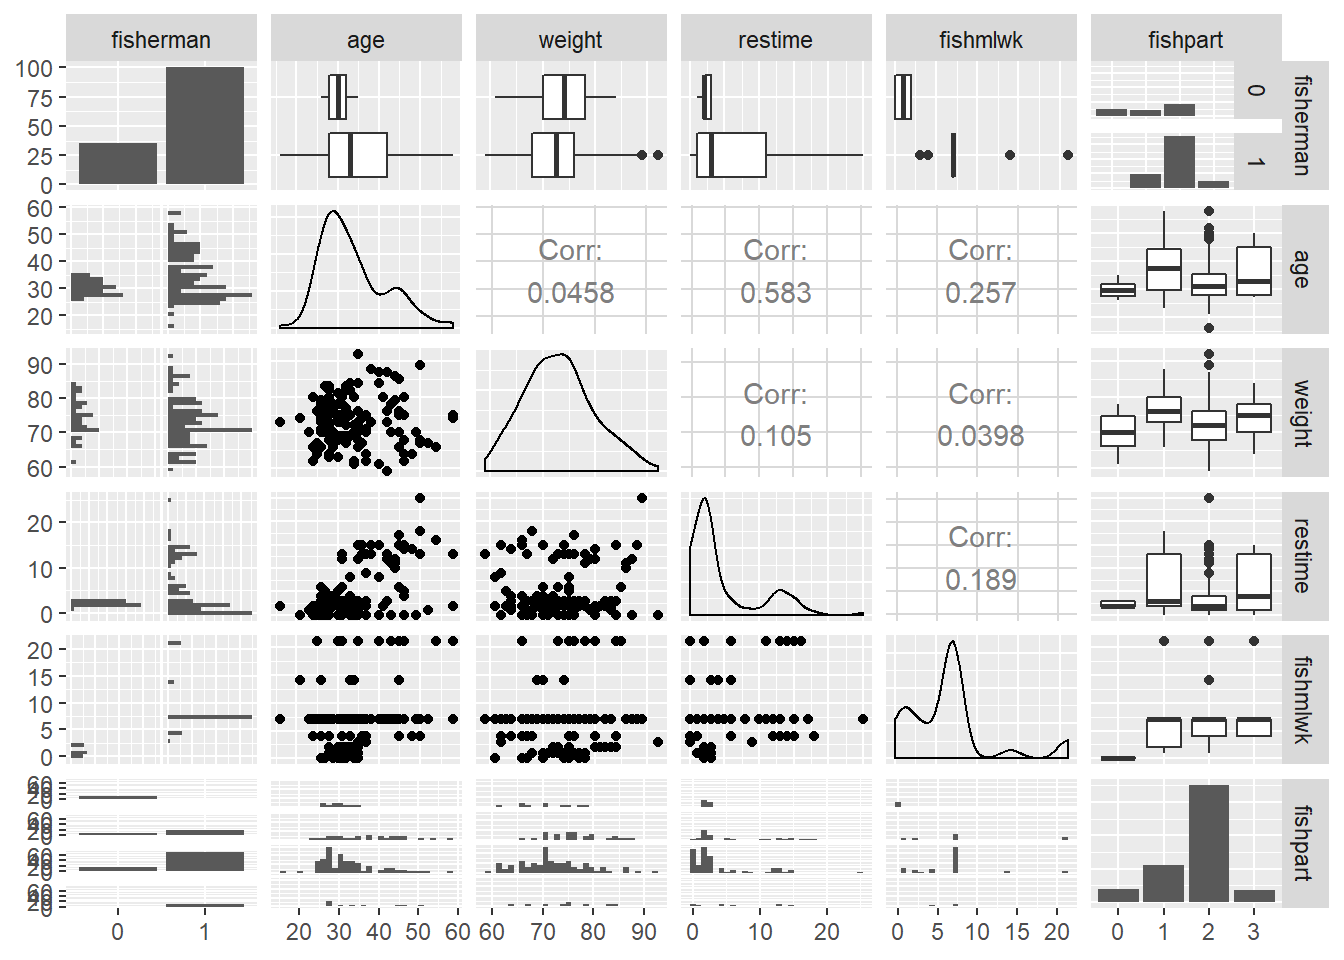
\includegraphics{Data_analysis_files/figure-latex/unnamed-chunk-6-1.pdf}

\begin{Shaded}
\begin{Highlighting}[]
\KeywordTok{ggpairs}\NormalTok{(dataset.fisherman[, }\KeywordTok{c}\NormalTok{(}\StringTok{"fisherman"}\NormalTok{, }\StringTok{"age"}\NormalTok{, }\StringTok{"weight"}\NormalTok{, }\StringTok{"restime"}\NormalTok{, }\StringTok{"fishmlwk"}\NormalTok{, }\StringTok{"fishpart"}\NormalTok{)])}
\end{Highlighting}
\end{Shaded}

\begin{verbatim}
## `stat_bin()` using `bins = 30`. Pick better value with `binwidth`.
## `stat_bin()` using `bins = 30`. Pick better value with `binwidth`.
## `stat_bin()` using `bins = 30`. Pick better value with `binwidth`.
## `stat_bin()` using `bins = 30`. Pick better value with `binwidth`.
## `stat_bin()` using `bins = 30`. Pick better value with `binwidth`.
## `stat_bin()` using `bins = 30`. Pick better value with `binwidth`.
## `stat_bin()` using `bins = 30`. Pick better value with `binwidth`.
## `stat_bin()` using `bins = 30`. Pick better value with `binwidth`.
\end{verbatim}

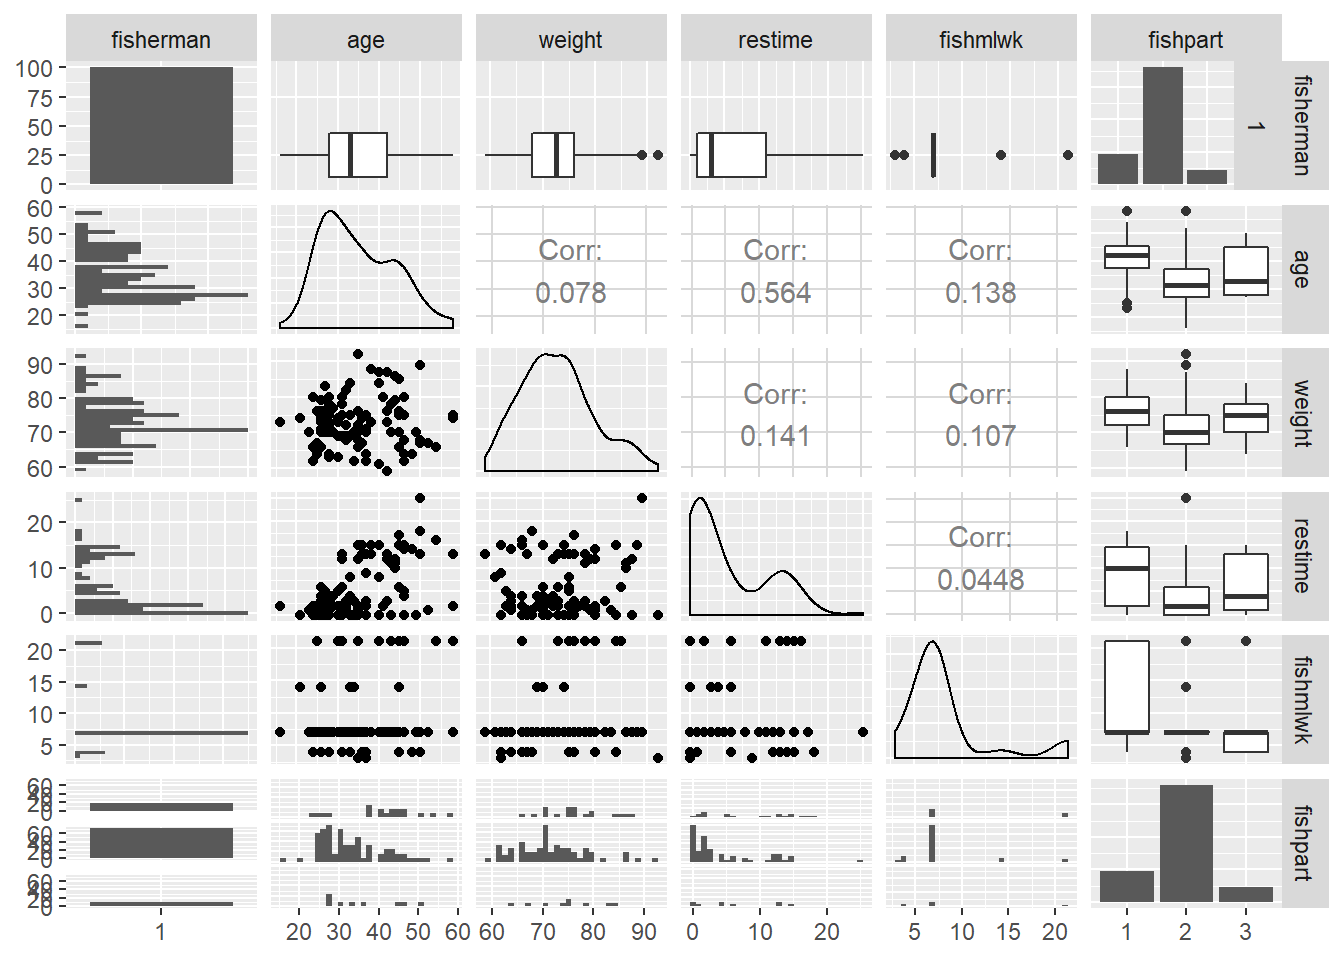
\includegraphics{Data_analysis_files/figure-latex/unnamed-chunk-6-2.pdf}

\begin{Shaded}
\begin{Highlighting}[]
\KeywordTok{ggpairs}\NormalTok{(dataset.non_fisherman[, }\KeywordTok{c}\NormalTok{(}\StringTok{"fisherman"}\NormalTok{, }\StringTok{"age"}\NormalTok{, }\StringTok{"weight"}\NormalTok{, }\StringTok{"restime"}\NormalTok{, }\StringTok{"fishmlwk"}\NormalTok{, }\StringTok{"fishpart"}\NormalTok{)])}
\end{Highlighting}
\end{Shaded}

\begin{verbatim}
## `stat_bin()` using `bins = 30`. Pick better value with `binwidth`.
## `stat_bin()` using `bins = 30`. Pick better value with `binwidth`.
## `stat_bin()` using `bins = 30`. Pick better value with `binwidth`.
## `stat_bin()` using `bins = 30`. Pick better value with `binwidth`.
## `stat_bin()` using `bins = 30`. Pick better value with `binwidth`.
## `stat_bin()` using `bins = 30`. Pick better value with `binwidth`.
## `stat_bin()` using `bins = 30`. Pick better value with `binwidth`.
## `stat_bin()` using `bins = 30`. Pick better value with `binwidth`.
\end{verbatim}

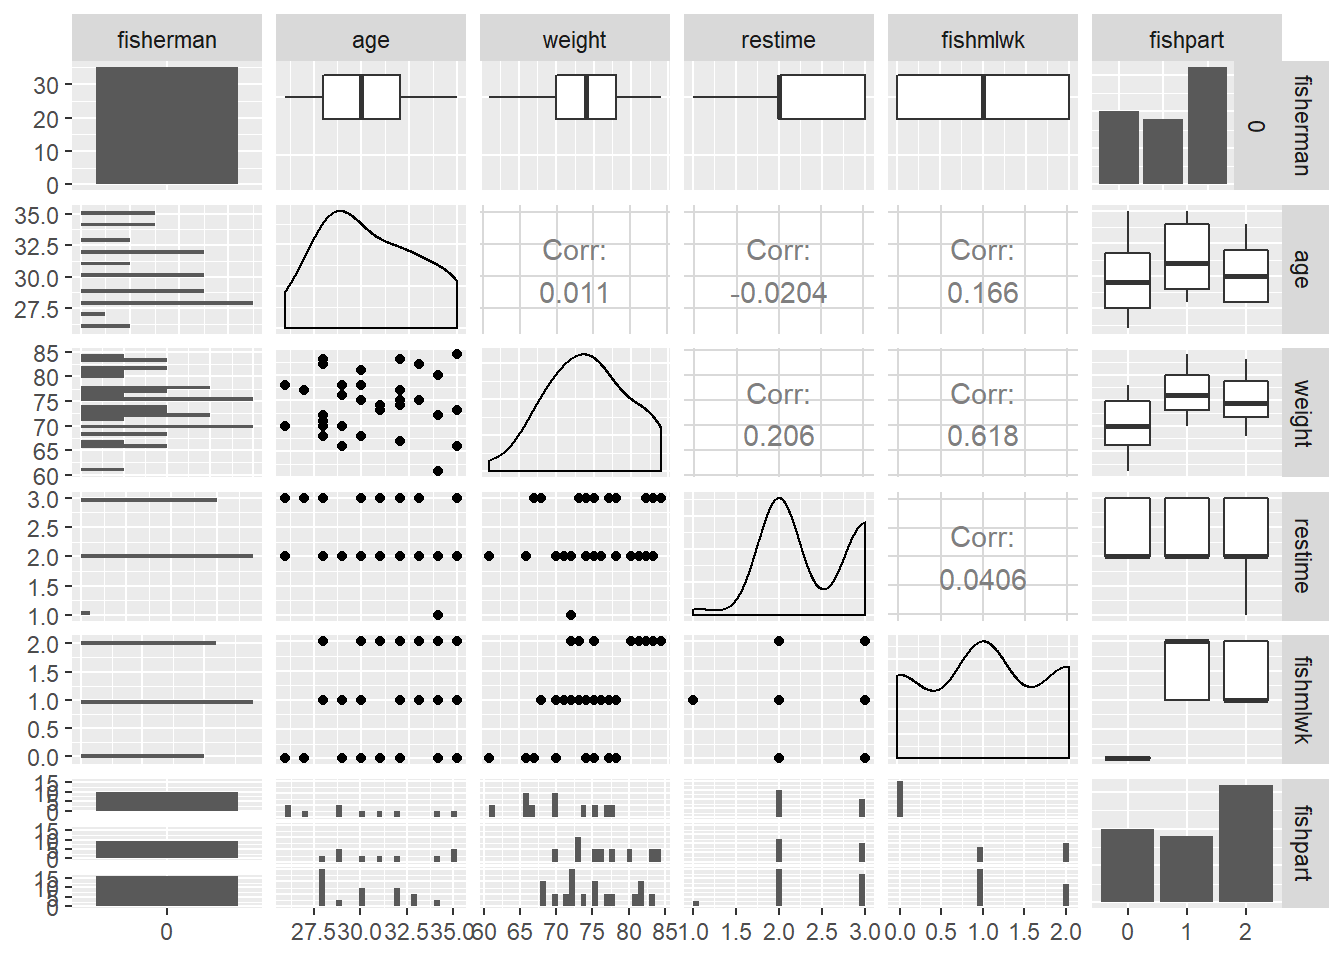
\includegraphics{Data_analysis_files/figure-latex/unnamed-chunk-6-3.pdf}

\subsubsection{Plots of factored data}\label{plots-of-factored-data}

\begin{Shaded}
\begin{Highlighting}[]
\KeywordTok{ggplot}\NormalTok{(dataset, }\KeywordTok{aes}\NormalTok{(fisherman, TotHg)) }\OperatorTok{+}\StringTok{ }\KeywordTok{geom_boxplot}\NormalTok{()}
\end{Highlighting}
\end{Shaded}

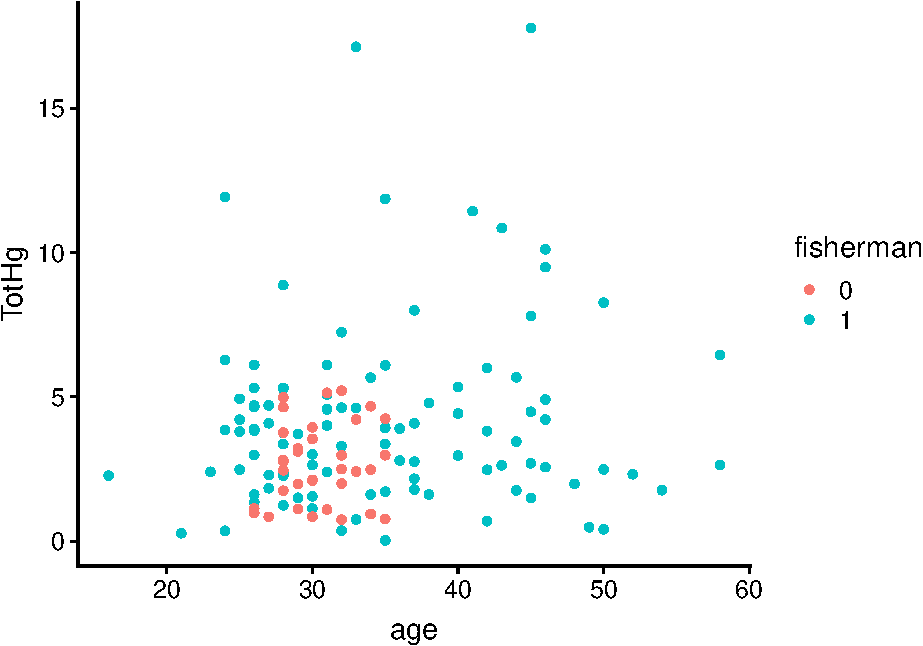
\includegraphics{Data_analysis_files/figure-latex/unnamed-chunk-7-1.pdf}

\begin{Shaded}
\begin{Highlighting}[]
\KeywordTok{ggplot}\NormalTok{(dataset, }\KeywordTok{aes}\NormalTok{(age, TotHg, }\DataTypeTok{colour =}\NormalTok{ fisherman)) }\OperatorTok{+}\StringTok{ }\KeywordTok{geom_point}\NormalTok{() }\CommentTok{#+ scale_y_log10() + scale_x_log10() ##Uncomment for log scales}
\end{Highlighting}
\end{Shaded}

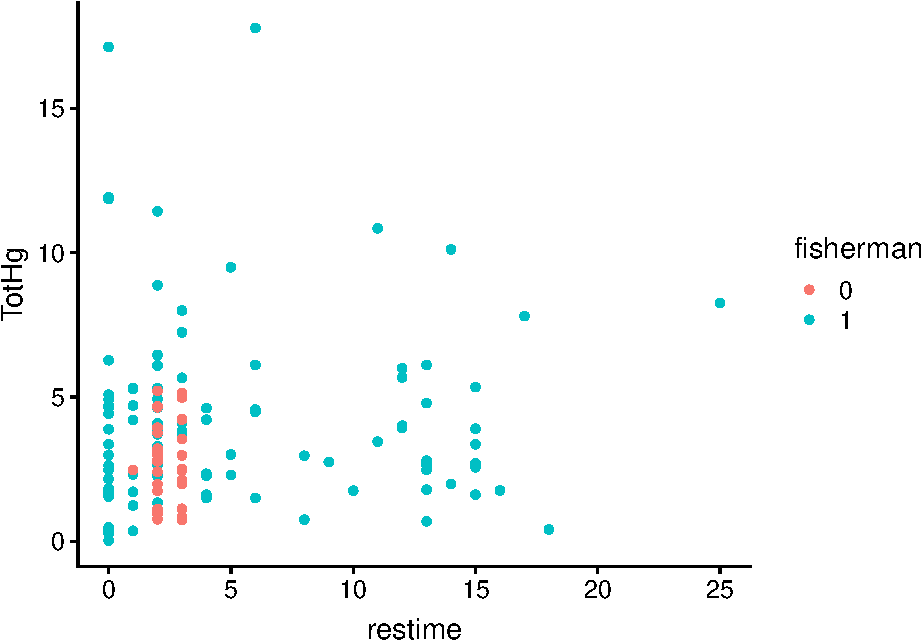
\includegraphics{Data_analysis_files/figure-latex/unnamed-chunk-7-2.pdf}

\begin{Shaded}
\begin{Highlighting}[]
\KeywordTok{ggplot}\NormalTok{(dataset, }\KeywordTok{aes}\NormalTok{(restime, TotHg, }\DataTypeTok{colour =}\NormalTok{ fisherman)) }\OperatorTok{+}\StringTok{ }\KeywordTok{geom_point}\NormalTok{()}
\end{Highlighting}
\end{Shaded}

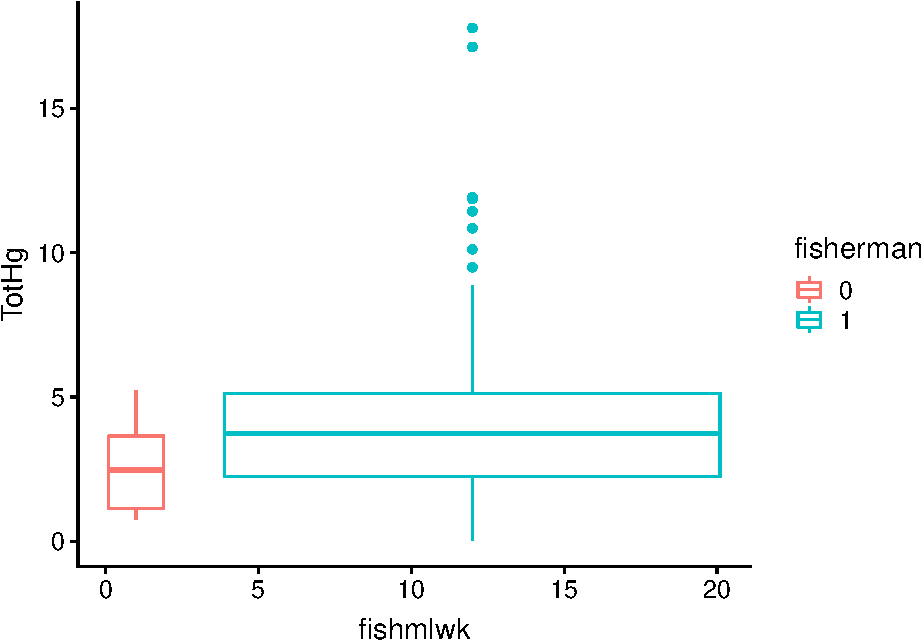
\includegraphics{Data_analysis_files/figure-latex/unnamed-chunk-7-3.pdf}

\begin{Shaded}
\begin{Highlighting}[]
\KeywordTok{ggplot}\NormalTok{(dataset, }\KeywordTok{aes}\NormalTok{(height, TotHg, }\DataTypeTok{colour =}\NormalTok{ fisherman)) }\OperatorTok{+}\StringTok{ }\KeywordTok{geom_point}\NormalTok{() }\CommentTok{#+ scale_y_log10() + scale_x_log10() }
\end{Highlighting}
\end{Shaded}

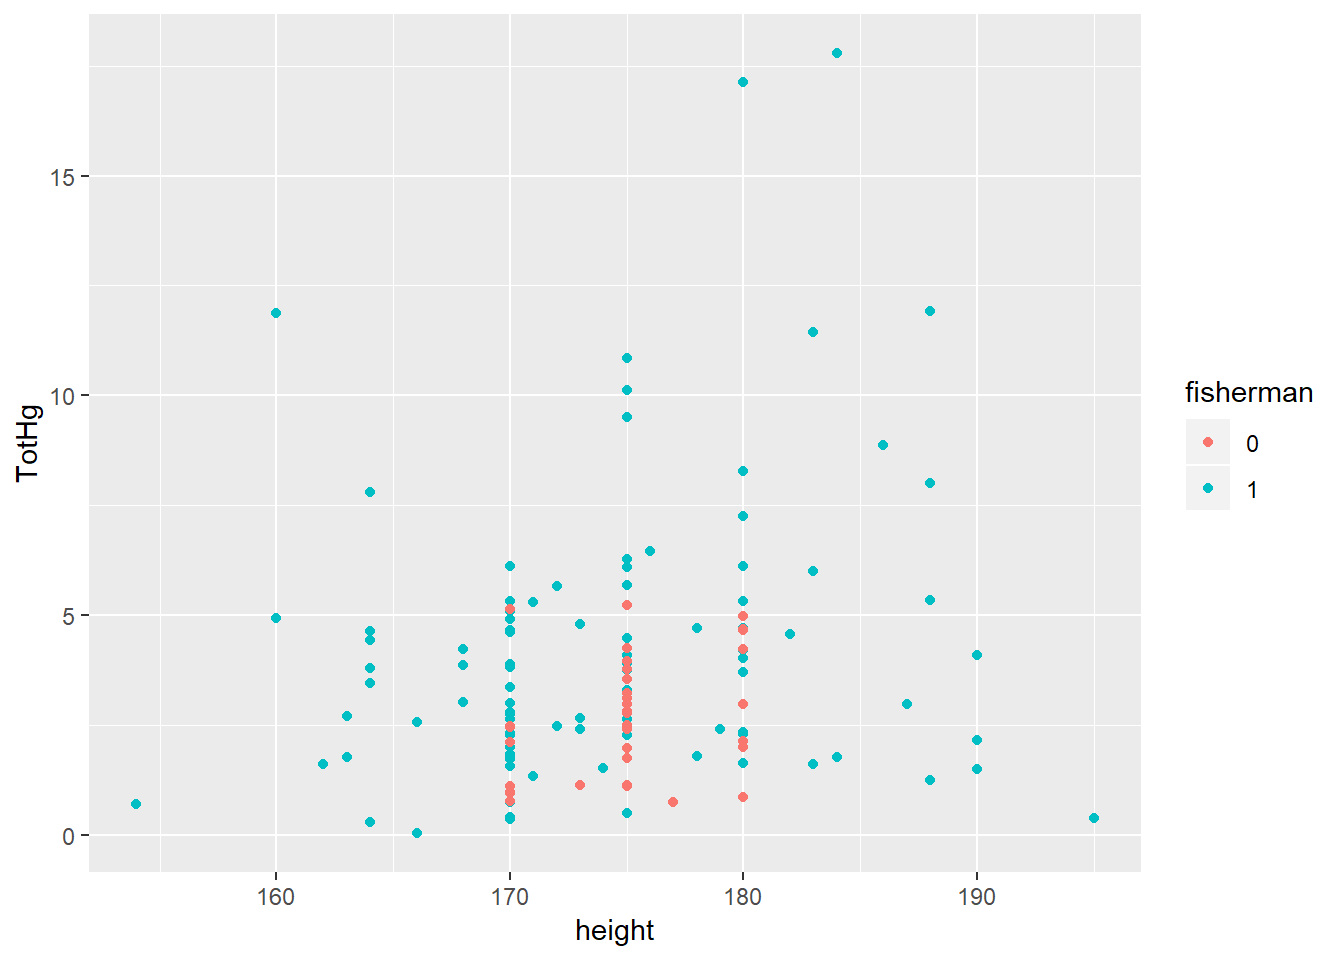
\includegraphics{Data_analysis_files/figure-latex/unnamed-chunk-7-4.pdf}

\begin{Shaded}
\begin{Highlighting}[]
\KeywordTok{ggplot}\NormalTok{(dataset, }\KeywordTok{aes}\NormalTok{(weight, TotHg, }\DataTypeTok{colour =}\NormalTok{ fisherman)) }\OperatorTok{+}\StringTok{ }\KeywordTok{geom_point}\NormalTok{() }\CommentTok{#+ scale_y_log10() + scale_x_log10()}
\end{Highlighting}
\end{Shaded}

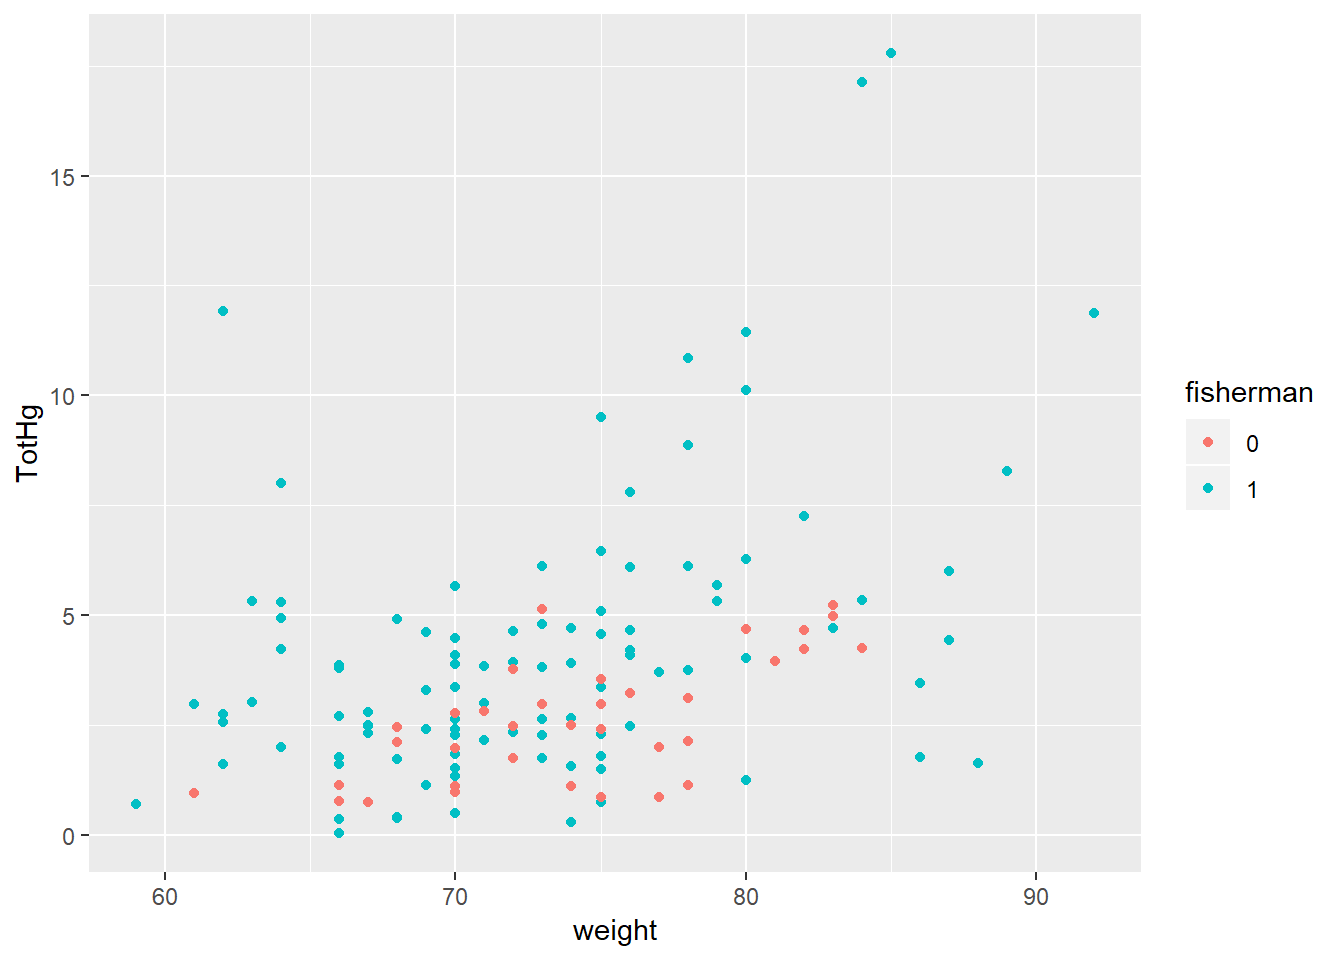
\includegraphics{Data_analysis_files/figure-latex/unnamed-chunk-7-5.pdf}

\begin{Shaded}
\begin{Highlighting}[]
\KeywordTok{ggplot}\NormalTok{(dataset, }\KeywordTok{aes}\NormalTok{(fishmlwk, TotHg, }\DataTypeTok{colour =}\NormalTok{ fisherman)) }\OperatorTok{+}\StringTok{ }\KeywordTok{geom_boxplot}\NormalTok{()}
\end{Highlighting}
\end{Shaded}

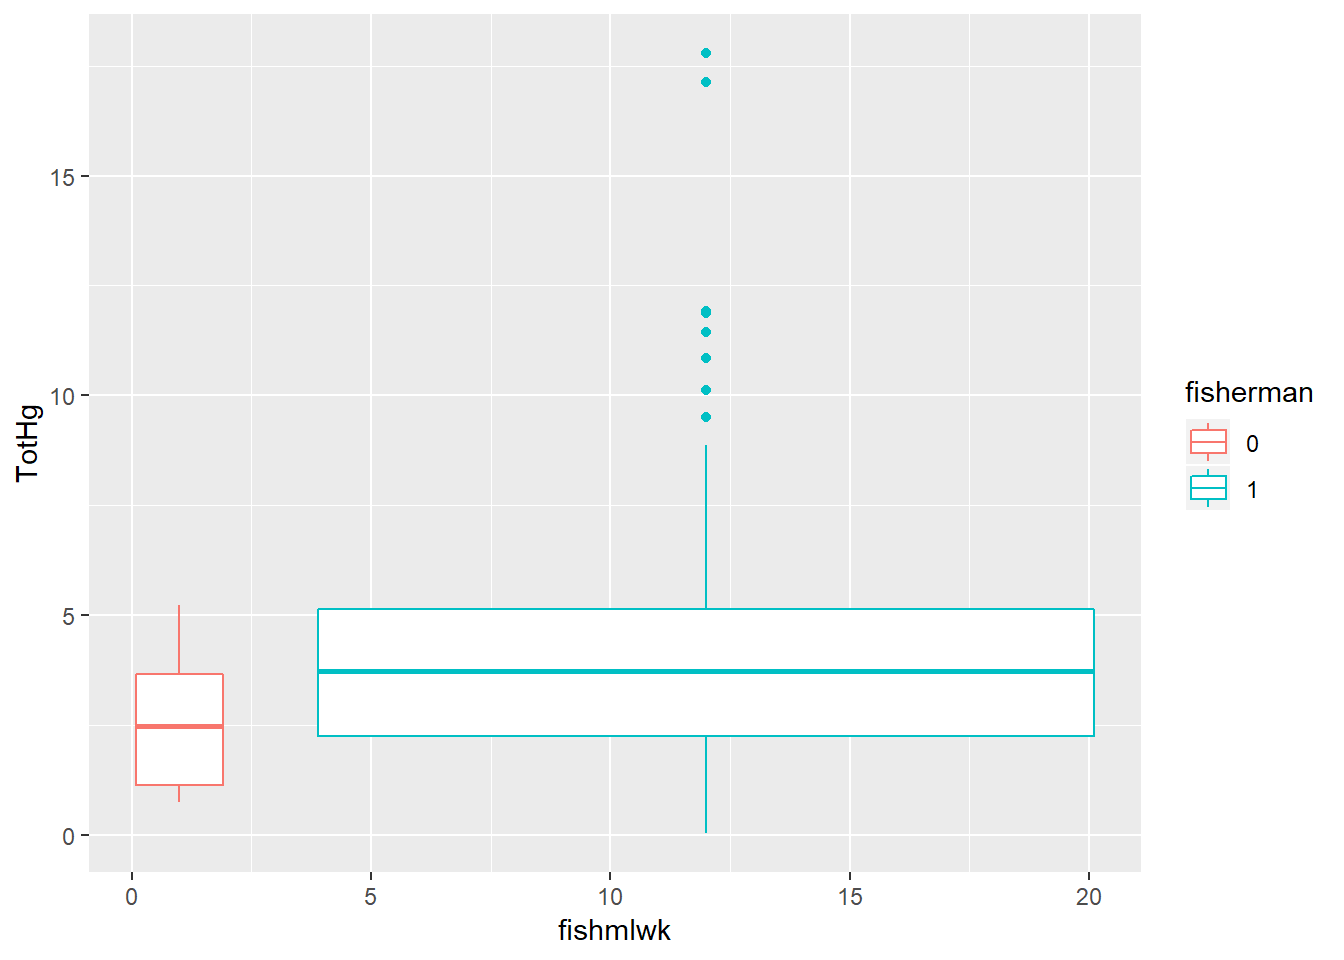
\includegraphics{Data_analysis_files/figure-latex/unnamed-chunk-7-6.pdf}

\begin{Shaded}
\begin{Highlighting}[]
\KeywordTok{ggplot}\NormalTok{(dataset, }\KeywordTok{aes}\NormalTok{(fishpart, TotHg, }\DataTypeTok{colour =}\NormalTok{ fisherman)) }\OperatorTok{+}\StringTok{ }\KeywordTok{geom_boxplot}\NormalTok{()}
\end{Highlighting}
\end{Shaded}

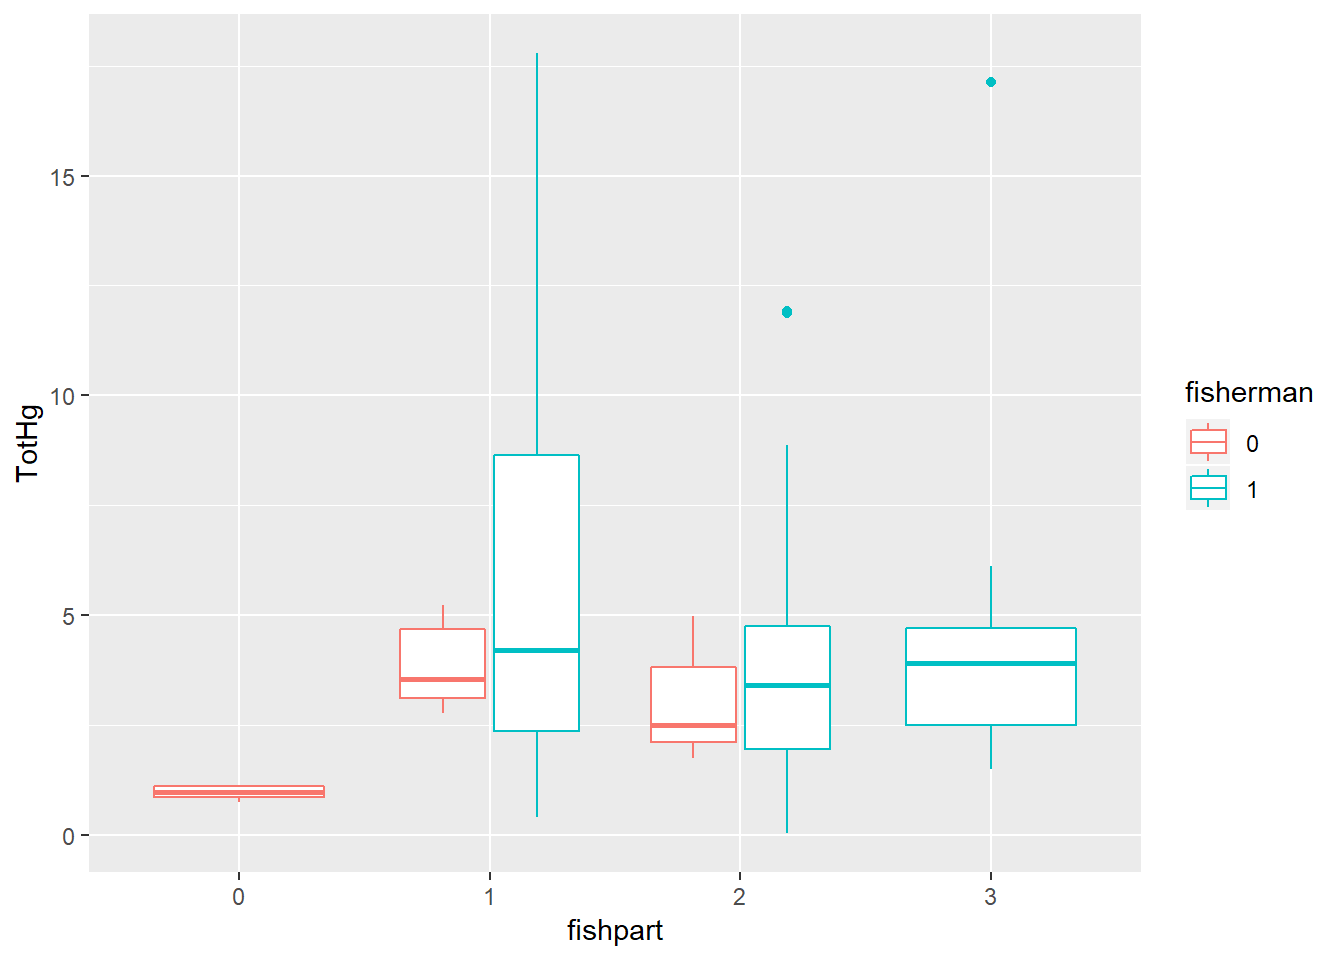
\includegraphics{Data_analysis_files/figure-latex/unnamed-chunk-7-7.pdf}

\subsection{Analyze}\label{analyze}

\subsubsection{1-D linear models}\label{d-linear-models}

\paragraph{Age}\label{age}

\subparagraph{Code}\label{code}

\begin{Shaded}
\begin{Highlighting}[]
\NormalTok{hg.form.age =}\StringTok{ }\NormalTok{TotHg }\OperatorTok{~}\StringTok{ }\NormalTok{age }\CommentTok{# 1-D regression}

\NormalTok{hg.lm.age =}\StringTok{ }\KeywordTok{lm}\NormalTok{(hg.form.age, }\DataTypeTok{data=}\NormalTok{dataset) }\CommentTok{# Whole population}
\NormalTok{hg.lmFi.age =}\StringTok{ }\KeywordTok{lm}\NormalTok{(hg.form.age, }\DataTypeTok{data=}\NormalTok{dataset.fisherman) }\CommentTok{# Fishermen population}
\NormalTok{hg.lmNF.age =}\StringTok{ }\KeywordTok{lm}\NormalTok{(hg.form.age, }\DataTypeTok{data=}\NormalTok{dataset.non_fisherman) }\CommentTok{# Control population}

\CommentTok{# Diagnostic plots}
\KeywordTok{par}\NormalTok{(}\DataTypeTok{mfrow=}\KeywordTok{c}\NormalTok{(}\DecValTok{2}\NormalTok{,}\DecValTok{2}\NormalTok{))}
\KeywordTok{plot}\NormalTok{(hg.lm.age)}
\KeywordTok{mtext}\NormalTok{(}\StringTok{"TotHg as a function of age - Whole population"}\NormalTok{, }\DataTypeTok{side =} \DecValTok{3}\NormalTok{, }\DataTypeTok{line =} \OperatorTok{-}\DecValTok{2}\NormalTok{, }\DataTypeTok{outer =} \OtherTok{TRUE}\NormalTok{, }\DataTypeTok{cex =} \FloatTok{1.5}\NormalTok{)}
\end{Highlighting}
\end{Shaded}

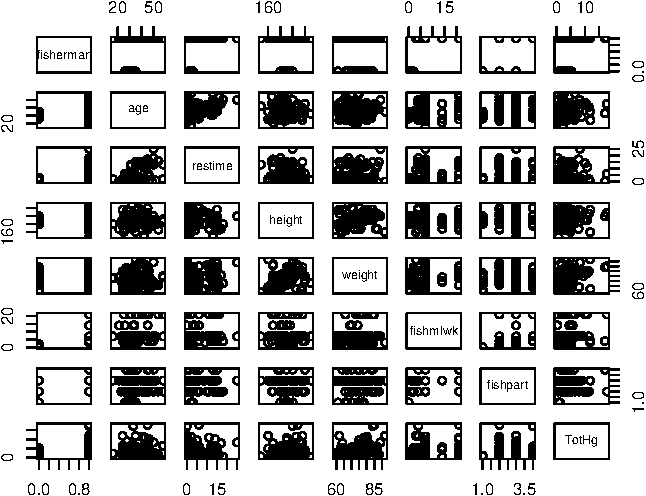
\includegraphics{Data_analysis_files/figure-latex/unnamed-chunk-8-1.pdf}

\begin{Shaded}
\begin{Highlighting}[]
\KeywordTok{par}\NormalTok{(}\DataTypeTok{mfrow=}\KeywordTok{c}\NormalTok{(}\DecValTok{2}\NormalTok{,}\DecValTok{2}\NormalTok{))}
\KeywordTok{plot}\NormalTok{(hg.lmFi.age)}
\KeywordTok{mtext}\NormalTok{(}\StringTok{"TotHg as a function of age - Fishermen population"}\NormalTok{, }\DataTypeTok{side =} \DecValTok{3}\NormalTok{, }\DataTypeTok{line =} \OperatorTok{-}\DecValTok{2}\NormalTok{, }\DataTypeTok{outer =} \OtherTok{TRUE}\NormalTok{, }\DataTypeTok{cex =} \FloatTok{1.5}\NormalTok{)}
\end{Highlighting}
\end{Shaded}

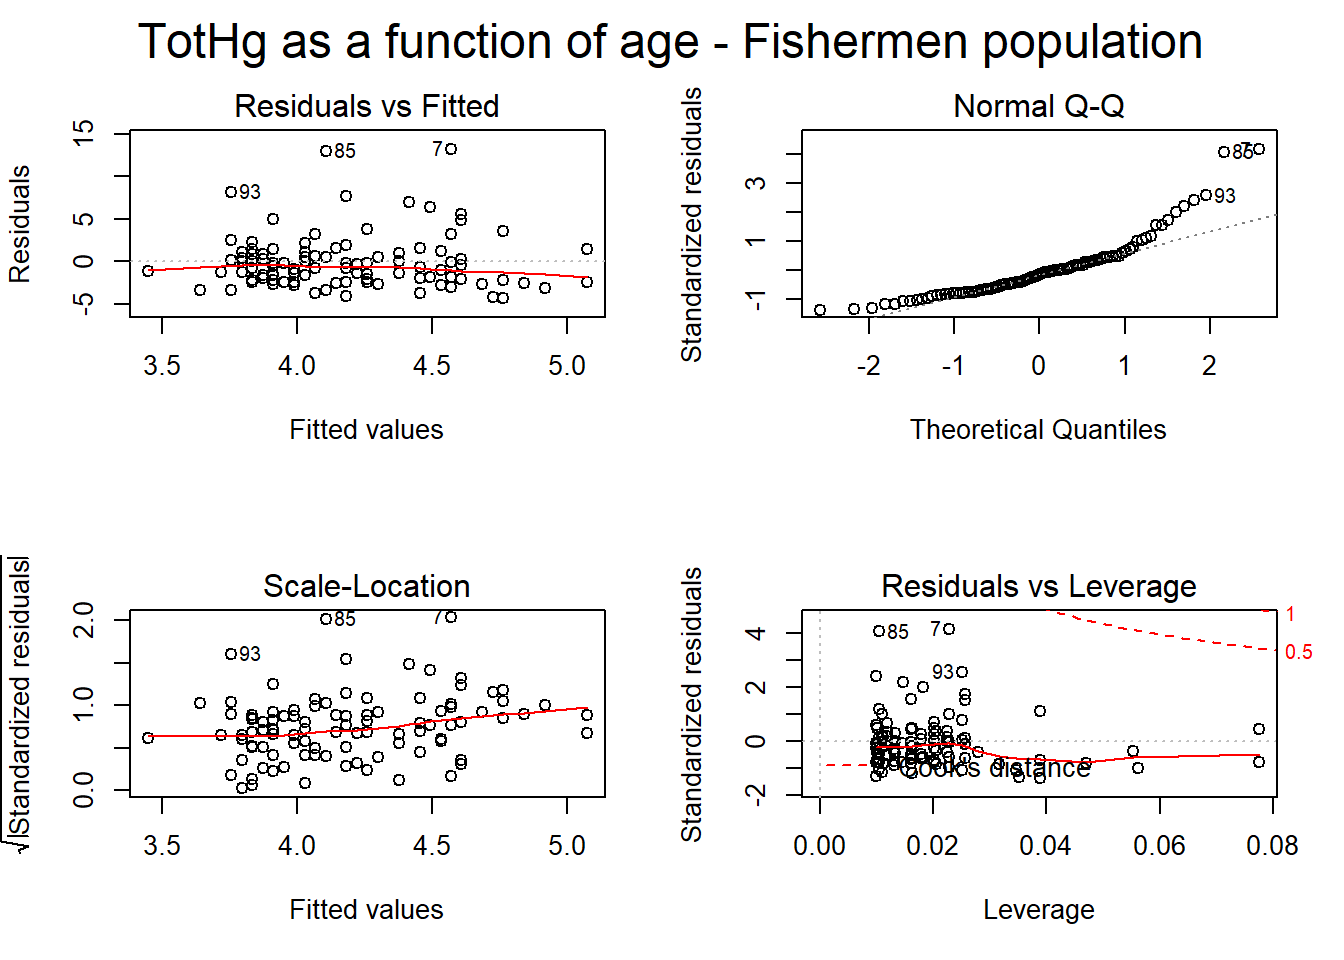
\includegraphics{Data_analysis_files/figure-latex/unnamed-chunk-8-2.pdf}

\begin{Shaded}
\begin{Highlighting}[]
\KeywordTok{par}\NormalTok{(}\DataTypeTok{mfrow=}\KeywordTok{c}\NormalTok{(}\DecValTok{2}\NormalTok{,}\DecValTok{2}\NormalTok{))}
\KeywordTok{plot}\NormalTok{(hg.lmNF.age)}
\KeywordTok{mtext}\NormalTok{(}\StringTok{"TotHg as a function of age - Non-Fishermen population"}\NormalTok{, }\DataTypeTok{side =} \DecValTok{3}\NormalTok{, }\DataTypeTok{line =} \OperatorTok{-}\DecValTok{2}\NormalTok{, }\DataTypeTok{outer =} \OtherTok{TRUE}\NormalTok{, }\DataTypeTok{cex =} \FloatTok{1.5}\NormalTok{)}
\end{Highlighting}
\end{Shaded}

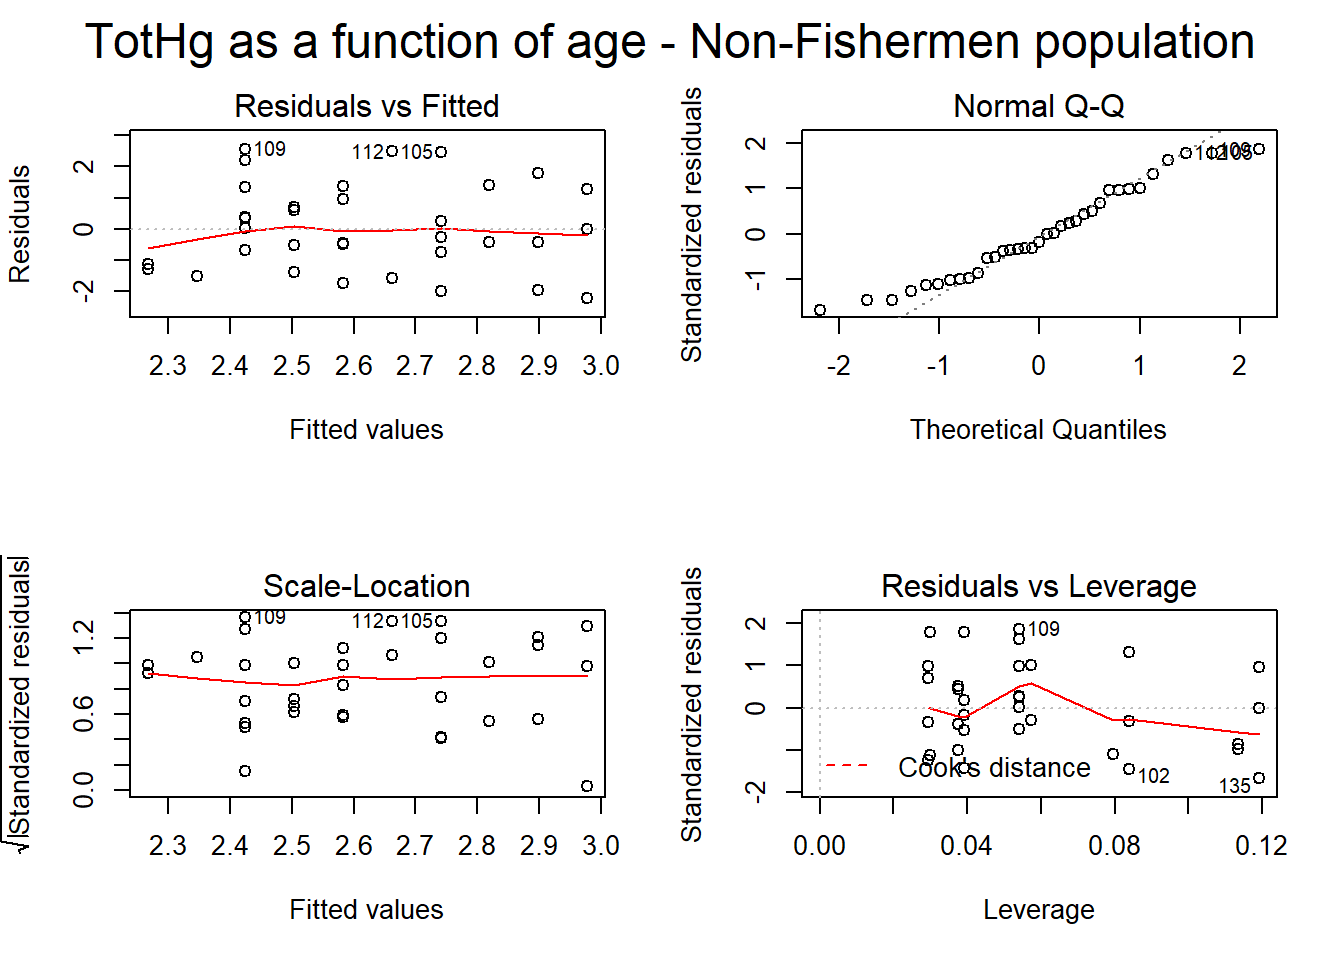
\includegraphics{Data_analysis_files/figure-latex/unnamed-chunk-8-3.pdf}

\subparagraph{Comments:}\label{comments}

\begin{itemize}
\tightlist
\item
  Residuals seem all in all well distributed in all three populations
  suggesting that the distribution of TotHg as a function of age is
  homoscedastic.
\item
  Normal Q-Q fits a line for Non-Fishermen population reinforcing the
  assumption that the distribution of TotHg given an age follows a
  normal distribution.
\item
  Normal Q-Q suggest however a heavy right tail for Fishermen population
  on this same distribution
\end{itemize}

\subparagraph{Test of homoskedasticity with a Breusch-Pagan test
(Joseph)}\label{test-of-homoskedasticity-with-a-breusch-pagan-test-joseph}

\begin{itemize}
\tightlist
\item
  This is a test for homoskedasticity of the data. The null hypothesis
  is homoskedasticity, and ncvTest calculates a p-value.
\end{itemize}

\begin{Shaded}
\begin{Highlighting}[]
\KeywordTok{ncvTest}\NormalTok{(hg.lm.age) }\CommentTok{# Output: Chisquare = 10.93327, Df = 1, p = 0.00094453}
\end{Highlighting}
\end{Shaded}

\begin{verbatim}
## Non-constant Variance Score Test 
## Variance formula: ~ fitted.values 
## Chisquare = 10.93327, Df = 1, p = 0.00094453
\end{verbatim}

\begin{Shaded}
\begin{Highlighting}[]
\KeywordTok{ncvTest}\NormalTok{(hg.lmFi.age) }\CommentTok{# Output: Chisquare = 4.561776, Df = 1, p = 0.032693}
\end{Highlighting}
\end{Shaded}

\begin{verbatim}
## Non-constant Variance Score Test 
## Variance formula: ~ fitted.values 
## Chisquare = 4.561776, Df = 1, p = 0.032693
\end{verbatim}

\begin{Shaded}
\begin{Highlighting}[]
\KeywordTok{ncvTest}\NormalTok{(hg.lmNF.age) }\CommentTok{# Output: Chisquare = 0.2004155, Df = 1, p = 0.65439}
\end{Highlighting}
\end{Shaded}

\begin{verbatim}
## Non-constant Variance Score Test 
## Variance formula: ~ fitted.values 
## Chisquare = 0.2004155, Df = 1, p = 0.65439
\end{verbatim}

These results suggest that only the non-Fisherman pop has homoskedastic
HgTot vs.~Age values.

\paragraph{Restime}\label{restime}

\subparagraph{Code}\label{code-1}

\begin{Shaded}
\begin{Highlighting}[]
\NormalTok{hg.form.restime =}\StringTok{ }\NormalTok{TotHg }\OperatorTok{~}\StringTok{ }\NormalTok{restime}

\NormalTok{hg.lm.restime =}\StringTok{ }\KeywordTok{lm}\NormalTok{(hg.form.restime, }\DataTypeTok{data=}\NormalTok{dataset)}
\NormalTok{hg.lmFi.restime =}\StringTok{ }\KeywordTok{lm}\NormalTok{(hg.form.restime, }\DataTypeTok{data=}\NormalTok{dataset.fisherman)}
\NormalTok{hg.lmNF.restime =}\StringTok{ }\KeywordTok{lm}\NormalTok{(hg.form.restime, }\DataTypeTok{data=}\NormalTok{dataset.non_fisherman)}

\KeywordTok{par}\NormalTok{(}\DataTypeTok{mfrow=}\KeywordTok{c}\NormalTok{(}\DecValTok{2}\NormalTok{,}\DecValTok{2}\NormalTok{))}
\KeywordTok{plot}\NormalTok{(hg.lm.restime)}
\KeywordTok{mtext}\NormalTok{(}\StringTok{"TotHg as a function of restime - Whole population"}\NormalTok{, }\DataTypeTok{side =} \DecValTok{3}\NormalTok{, }\DataTypeTok{line =} \OperatorTok{-}\DecValTok{2}\NormalTok{, }\DataTypeTok{outer =} \OtherTok{TRUE}\NormalTok{, }\DataTypeTok{cex =} \FloatTok{1.5}\NormalTok{)}
\end{Highlighting}
\end{Shaded}

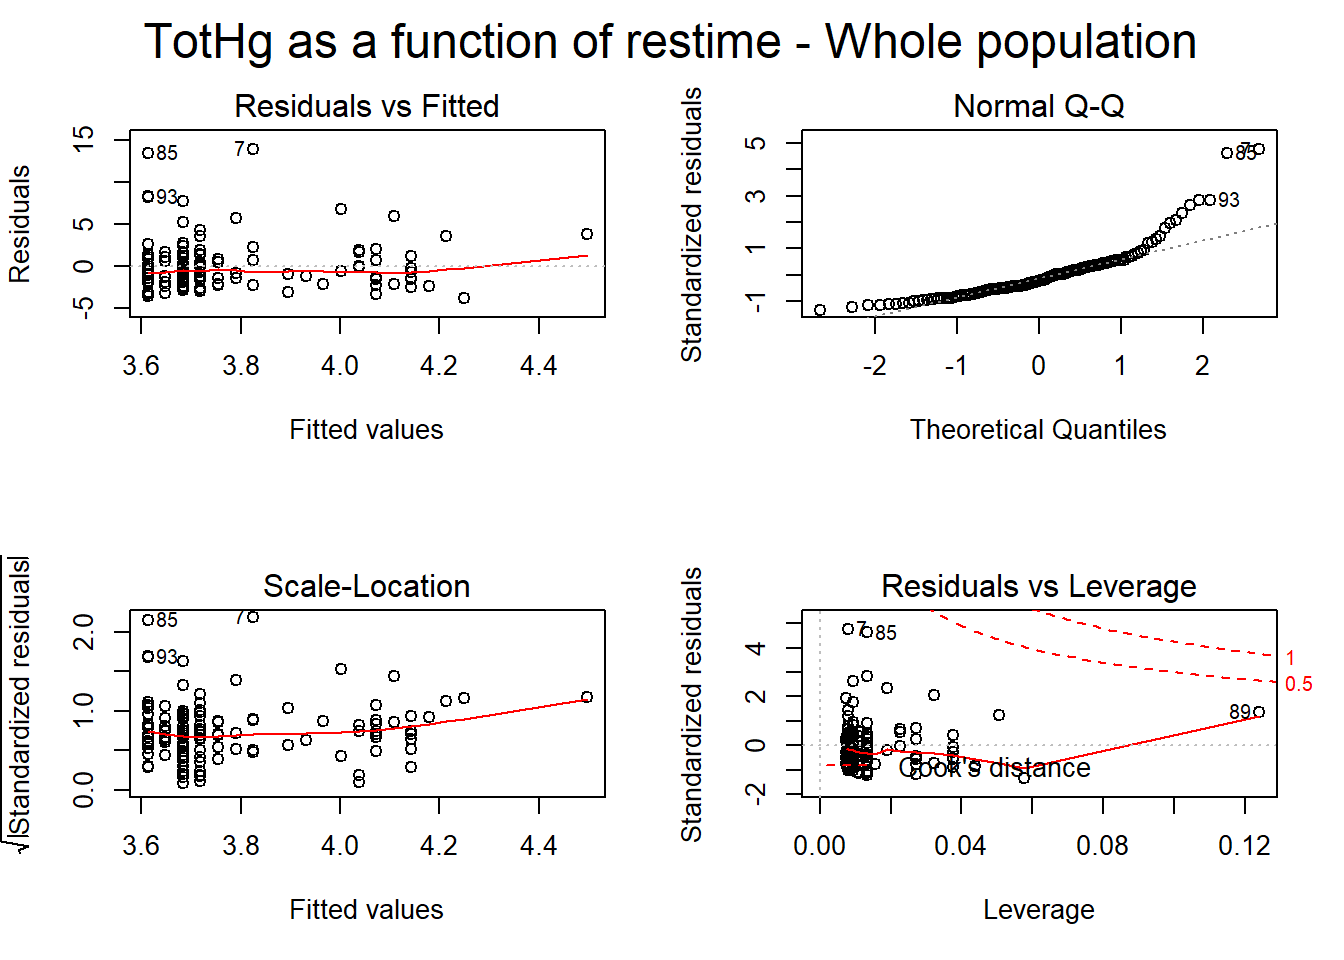
\includegraphics{Data_analysis_files/figure-latex/unnamed-chunk-10-1.pdf}

\begin{Shaded}
\begin{Highlighting}[]
\KeywordTok{par}\NormalTok{(}\DataTypeTok{mfrow=}\KeywordTok{c}\NormalTok{(}\DecValTok{2}\NormalTok{,}\DecValTok{2}\NormalTok{))}
\KeywordTok{plot}\NormalTok{(hg.lmFi.restime)}
\KeywordTok{mtext}\NormalTok{(}\StringTok{"TotHg as a function of restime - Fishermen population"}\NormalTok{, }\DataTypeTok{side =} \DecValTok{3}\NormalTok{, }\DataTypeTok{line =} \OperatorTok{-}\DecValTok{2}\NormalTok{, }\DataTypeTok{outer =} \OtherTok{TRUE}\NormalTok{, }\DataTypeTok{cex =} \FloatTok{1.5}\NormalTok{)}
\end{Highlighting}
\end{Shaded}

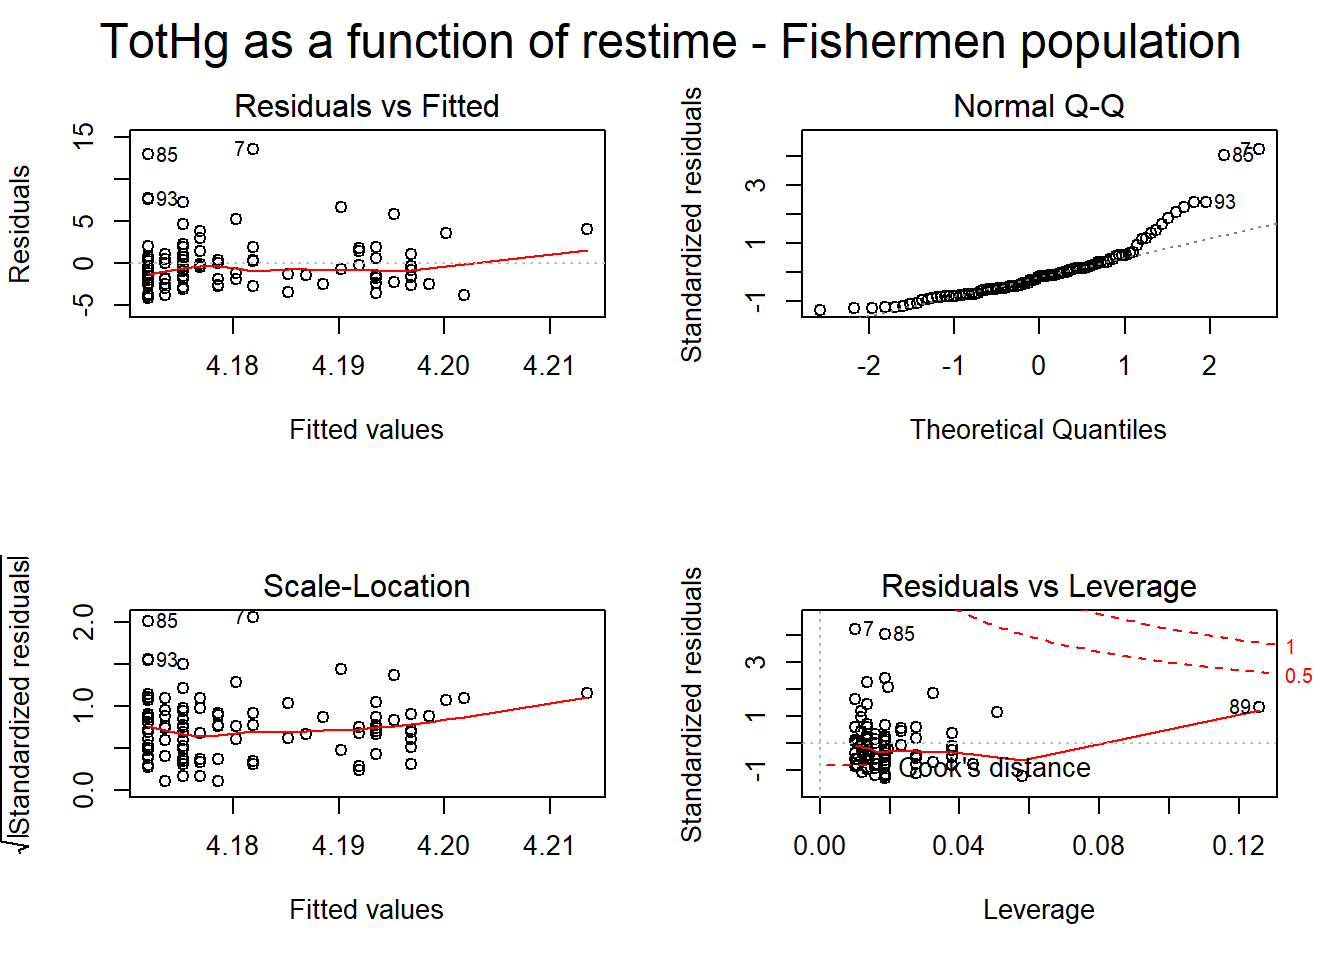
\includegraphics{Data_analysis_files/figure-latex/unnamed-chunk-10-2.pdf}

\begin{Shaded}
\begin{Highlighting}[]
\KeywordTok{par}\NormalTok{(}\DataTypeTok{mfrow=}\KeywordTok{c}\NormalTok{(}\DecValTok{2}\NormalTok{,}\DecValTok{2}\NormalTok{))}
\KeywordTok{plot}\NormalTok{(hg.lmNF.restime)}
\KeywordTok{mtext}\NormalTok{(}\StringTok{"TotHg as a function of restime - Non-Fishermen population"}\NormalTok{, }\DataTypeTok{side =} \DecValTok{3}\NormalTok{, }\DataTypeTok{line =} \OperatorTok{-}\DecValTok{2}\NormalTok{, }\DataTypeTok{outer =} \OtherTok{TRUE}\NormalTok{, }\DataTypeTok{cex =} \FloatTok{1.5}\NormalTok{)}
\end{Highlighting}
\end{Shaded}

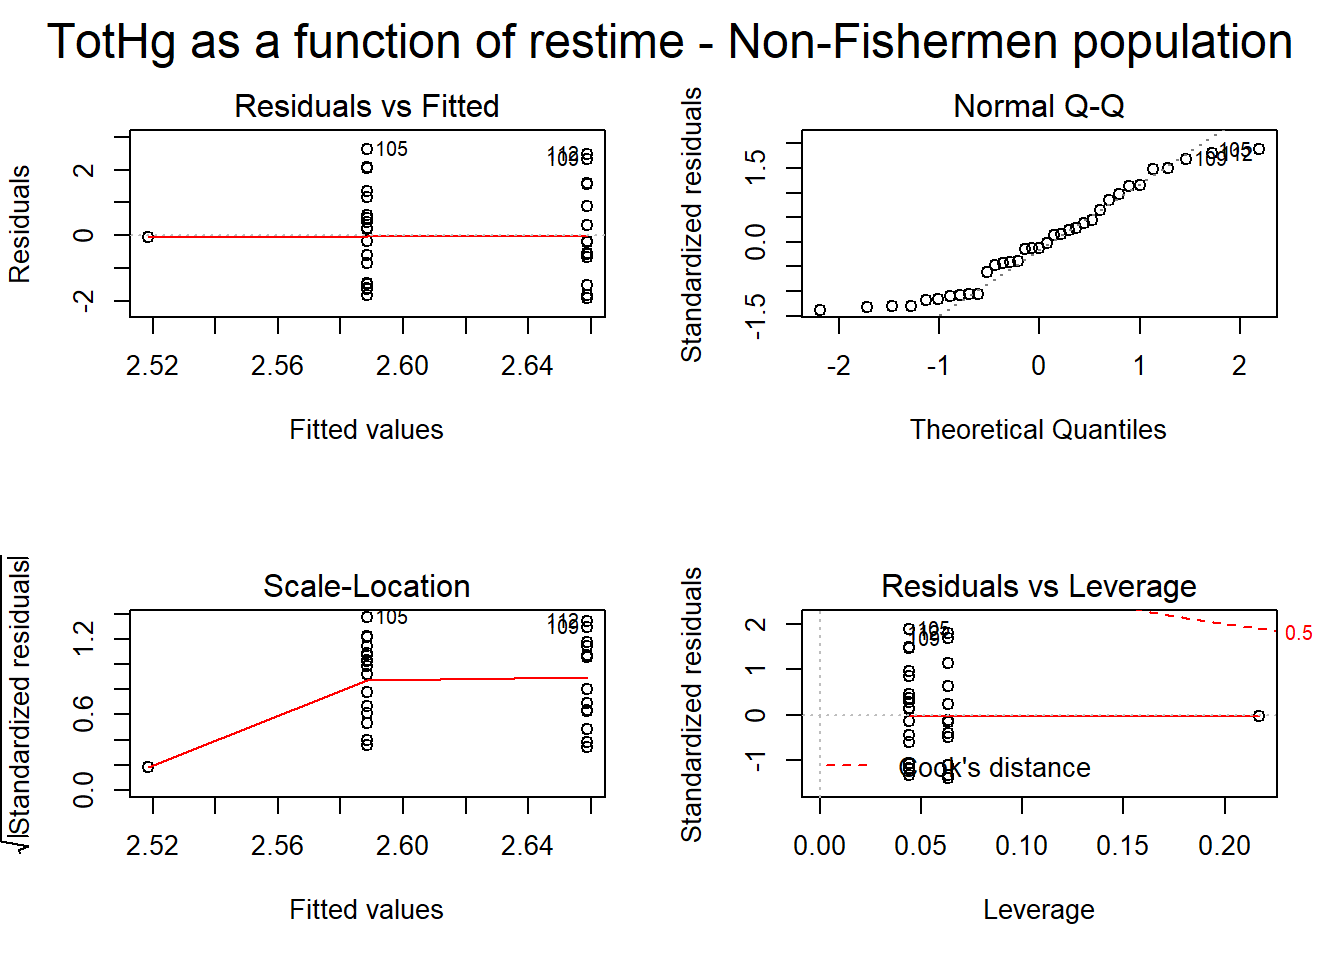
\includegraphics{Data_analysis_files/figure-latex/unnamed-chunk-10-3.pdf}

\subparagraph{Comments}\label{comments-1}

\begin{itemize}
\item
  There is a great difference of the distribution of \emph{restime}
  between Fishermen and control population. In the control population it
  takes a complete range of values whereas in the control population,
  the distribution is discrete and takes only 3 (even 2) different
  values. Thus it might be difficult to draw conclusions on whether
  \emph{restime} is correlated or not with the \emph{TotHg} value.
\item
  There also is this problem in Fishermen population of the right long
  tail and the left short tail for \emph{TotHg} distribution. \textbf{It
  might be useful to use a log scale.}
\item
  Residuals in Fishermen population for fitted \emph{TotHg} as a
  function of \emph{restime} are all in all well distributed around 0
  for all values of \emph{restime} suggesting an homoscedasticity of the
  distribution of \emph{TotHg} according to \emph{restime}.
\item
  However, there are some residuals with very high positive values when
  there are none with very ``high'' negative values, suggesting some
  possible bias in the distribution.
\end{itemize}

\subparagraph{Test of homoskedasticity with a Breusch-Pagan test
(Joseph)}\label{test-of-homoskedasticity-with-a-breusch-pagan-test-joseph-1}

\begin{itemize}
\tightlist
\item
  This is a test for homoskedasticity of the data. The null hypothesis
  is homoskedasticity, and ncvTest calculates a p-value.
\end{itemize}

\begin{Shaded}
\begin{Highlighting}[]
\KeywordTok{ncvTest}\NormalTok{(hg.lm.restime ) }\CommentTok{# Output: Chisquare = 0.2252327, Df = 1, p = 0.63508}
\end{Highlighting}
\end{Shaded}

\begin{verbatim}
## Non-constant Variance Score Test 
## Variance formula: ~ fitted.values 
## Chisquare = 0.2252327, Df = 1, p = 0.63508
\end{verbatim}

\begin{Shaded}
\begin{Highlighting}[]
\KeywordTok{ncvTest}\NormalTok{(hg.lmFi.restime ) }\CommentTok{# Output: Chisquare = 0.9487475, Df = 1, p = 0.33004}
\end{Highlighting}
\end{Shaded}

\begin{verbatim}
## Non-constant Variance Score Test 
## Variance formula: ~ fitted.values 
## Chisquare = 0.9487475, Df = 1, p = 0.33004
\end{verbatim}

\begin{Shaded}
\begin{Highlighting}[]
\KeywordTok{ncvTest}\NormalTok{(hg.lmNF.restime ) }\CommentTok{# Output: Chisquare = 0.2388775, Df = 1, p = 0.62502}
\end{Highlighting}
\end{Shaded}

\begin{verbatim}
## Non-constant Variance Score Test 
## Variance formula: ~ fitted.values 
## Chisquare = 0.2388775, Df = 1, p = 0.62502
\end{verbatim}

This time those results suggest that all 3 pop have homoskedastic HgTot
vs.~restime values.

\paragraph{LogWeight}\label{logweight}

\begin{Shaded}
\begin{Highlighting}[]
\NormalTok{hg.form.logWeight =}\StringTok{ }\NormalTok{LogTotHg }\OperatorTok{~}\StringTok{ }\NormalTok{weight}

\NormalTok{hg.lm.logWeight =}\StringTok{ }\KeywordTok{lm}\NormalTok{(hg.form.logWeight, }\DataTypeTok{data=}\NormalTok{dataset)}
\NormalTok{hg.lmFi.logWeight =}\StringTok{ }\KeywordTok{lm}\NormalTok{(hg.form.logWeight, }\DataTypeTok{data=}\NormalTok{dataset.fisherman)}
\NormalTok{hg.lmNF.logWeight =}\StringTok{ }\KeywordTok{lm}\NormalTok{(hg.form.logWeight, }\DataTypeTok{data=}\NormalTok{dataset.non_fisherman)}

\KeywordTok{par}\NormalTok{(}\DataTypeTok{mfrow=}\KeywordTok{c}\NormalTok{(}\DecValTok{2}\NormalTok{,}\DecValTok{2}\NormalTok{))}
\KeywordTok{plot}\NormalTok{(hg.lm.logWeight)}
\KeywordTok{mtext}\NormalTok{(}\StringTok{"LogTotHg as a function of weight - Whole population"}\NormalTok{, }\DataTypeTok{side =} \DecValTok{3}\NormalTok{, }\DataTypeTok{line =} \OperatorTok{-}\DecValTok{2}\NormalTok{, }\DataTypeTok{outer =} \OtherTok{TRUE}\NormalTok{, }\DataTypeTok{cex =} \FloatTok{1.5}\NormalTok{)}
\end{Highlighting}
\end{Shaded}

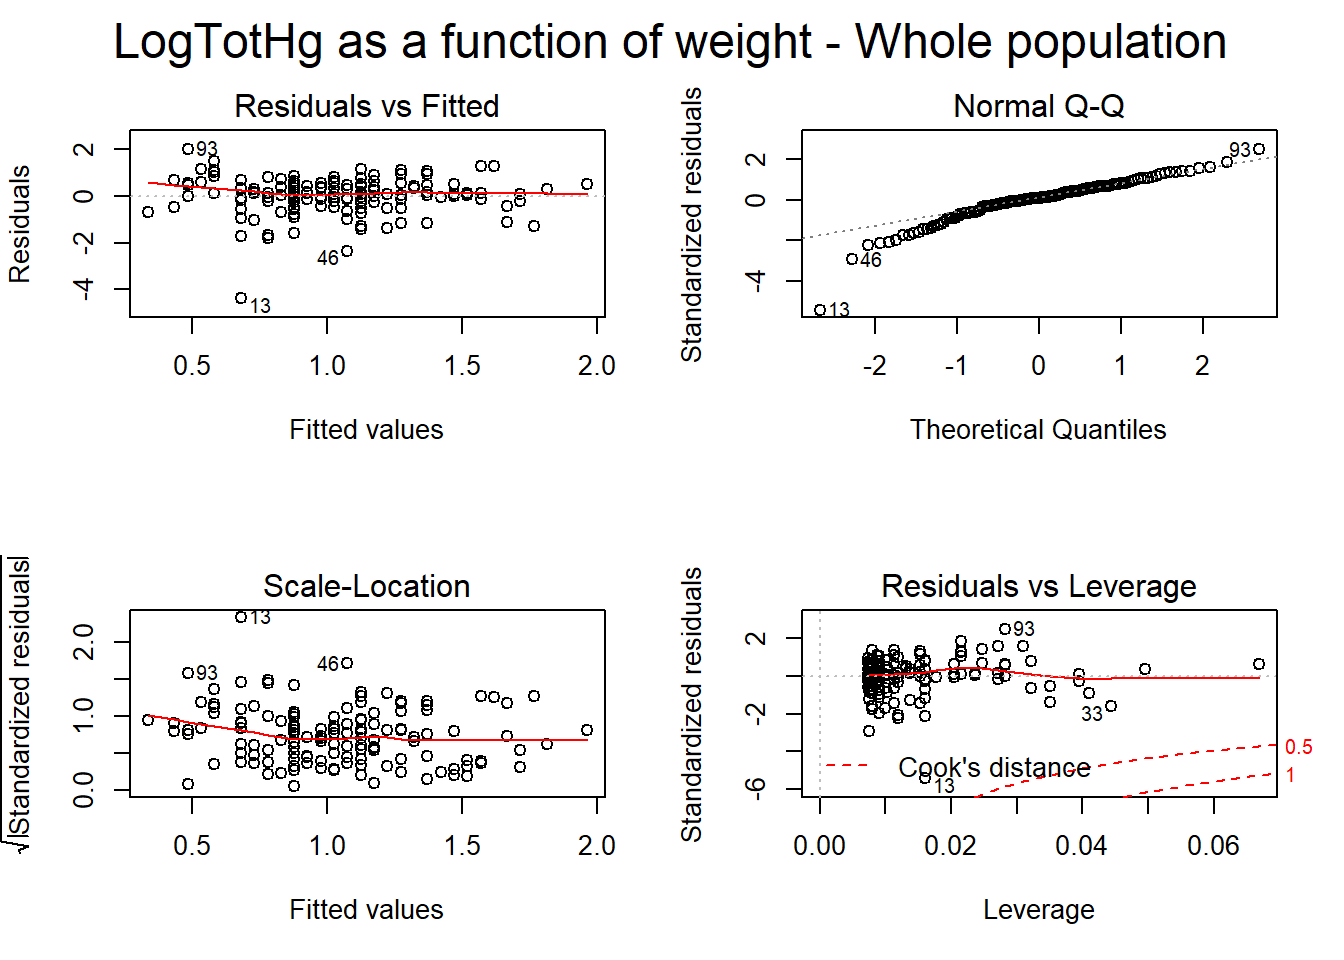
\includegraphics{Data_analysis_files/figure-latex/unnamed-chunk-12-1.pdf}

\begin{Shaded}
\begin{Highlighting}[]
\KeywordTok{par}\NormalTok{(}\DataTypeTok{mfrow=}\KeywordTok{c}\NormalTok{(}\DecValTok{2}\NormalTok{,}\DecValTok{2}\NormalTok{))}
\KeywordTok{plot}\NormalTok{(hg.lmFi.logWeight)}
\KeywordTok{mtext}\NormalTok{(}\StringTok{"LogTotHg as a function of weight - Fishermen population"}\NormalTok{, }\DataTypeTok{side =} \DecValTok{3}\NormalTok{, }\DataTypeTok{line =} \OperatorTok{-}\DecValTok{2}\NormalTok{, }\DataTypeTok{outer =} \OtherTok{TRUE}\NormalTok{, }\DataTypeTok{cex =} \FloatTok{1.5}\NormalTok{)}
\end{Highlighting}
\end{Shaded}

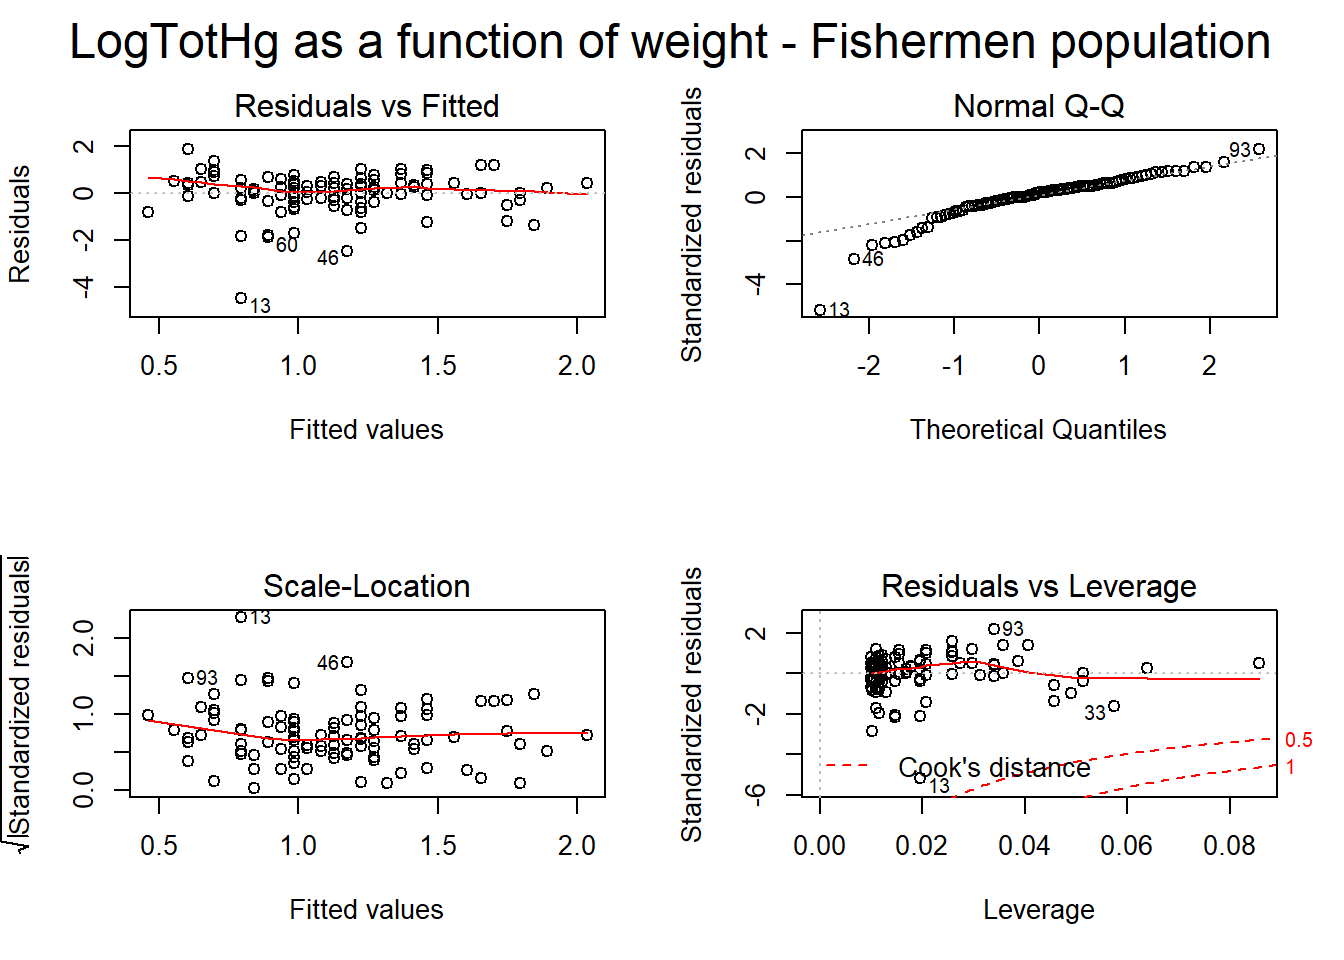
\includegraphics{Data_analysis_files/figure-latex/unnamed-chunk-12-2.pdf}

\begin{Shaded}
\begin{Highlighting}[]
\KeywordTok{par}\NormalTok{(}\DataTypeTok{mfrow=}\KeywordTok{c}\NormalTok{(}\DecValTok{2}\NormalTok{,}\DecValTok{2}\NormalTok{))}
\KeywordTok{plot}\NormalTok{(hg.lmNF.logWeight)}
\KeywordTok{mtext}\NormalTok{(}\StringTok{"LogTotHg as a function of weight - Non-Fishermen population"}\NormalTok{, }\DataTypeTok{side =} \DecValTok{3}\NormalTok{, }\DataTypeTok{line =} \OperatorTok{-}\DecValTok{2}\NormalTok{, }\DataTypeTok{outer =} \OtherTok{TRUE}\NormalTok{, }\DataTypeTok{cex =} \FloatTok{1.5}\NormalTok{)}
\end{Highlighting}
\end{Shaded}

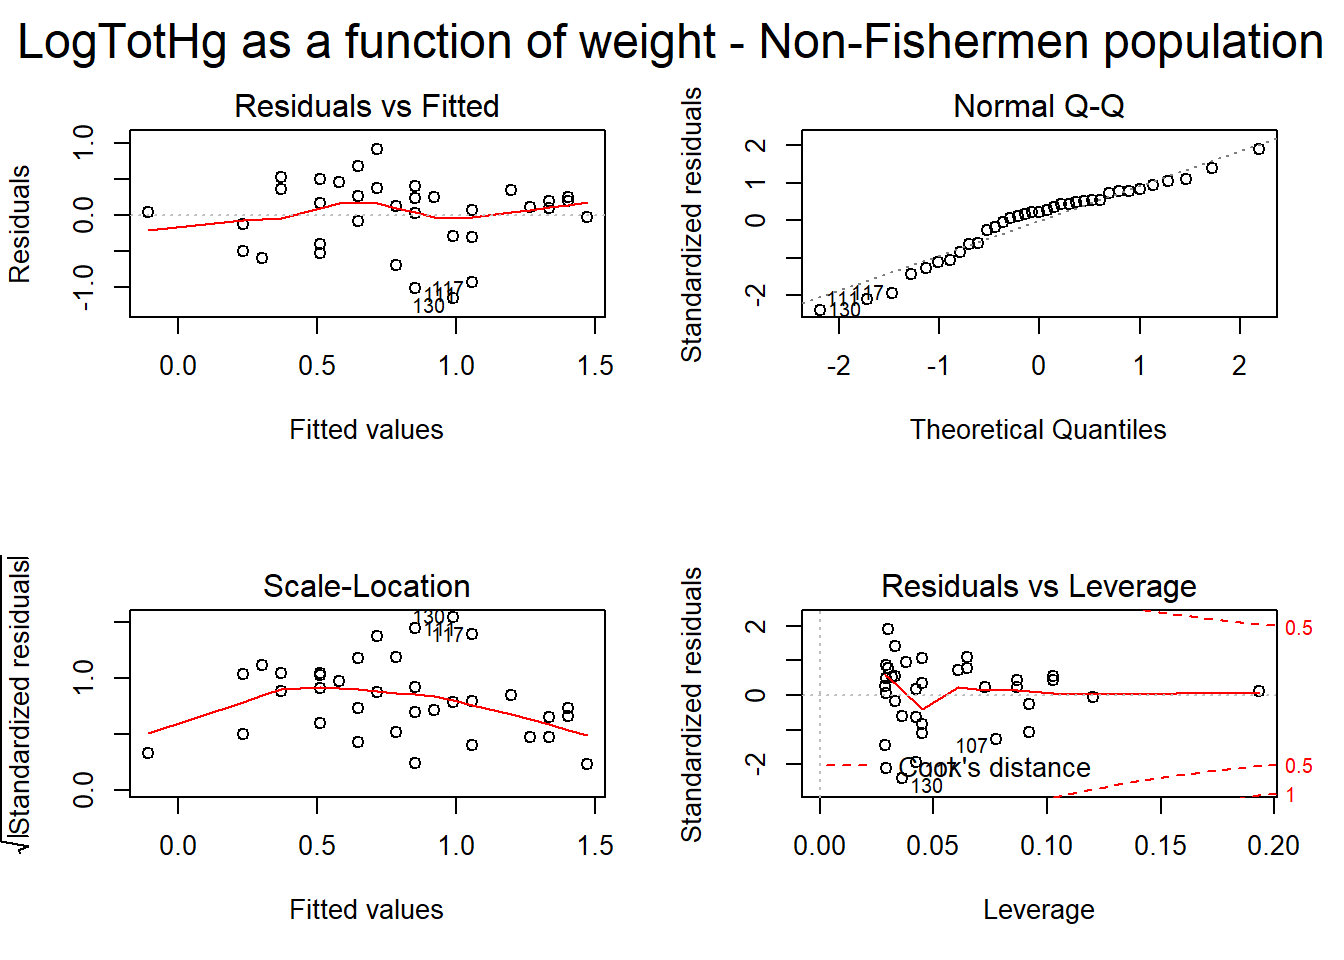
\includegraphics{Data_analysis_files/figure-latex/unnamed-chunk-12-3.pdf}

\paragraph{Weight}\label{weight}

\subparagraph{Code}\label{code-2}

\begin{Shaded}
\begin{Highlighting}[]
\NormalTok{hg.form.weight =}\StringTok{ }\NormalTok{TotHg }\OperatorTok{~}\StringTok{ }\NormalTok{weight}

\NormalTok{hg.lm.weight =}\StringTok{ }\KeywordTok{lm}\NormalTok{(hg.form.weight, }\DataTypeTok{data=}\NormalTok{dataset)}
\NormalTok{hg.lmFi.weight =}\StringTok{ }\KeywordTok{lm}\NormalTok{(hg.form.weight, }\DataTypeTok{data=}\NormalTok{dataset.fisherman)}
\NormalTok{hg.lmNF.weight =}\StringTok{ }\KeywordTok{lm}\NormalTok{(hg.form.weight, }\DataTypeTok{data=}\NormalTok{dataset.non_fisherman)}

\KeywordTok{par}\NormalTok{(}\DataTypeTok{mfrow=}\KeywordTok{c}\NormalTok{(}\DecValTok{2}\NormalTok{,}\DecValTok{2}\NormalTok{))}
\KeywordTok{plot}\NormalTok{(hg.lm.weight)}
\KeywordTok{mtext}\NormalTok{(}\StringTok{"TotHg as a function of weight - Whole population"}\NormalTok{, }\DataTypeTok{side =} \DecValTok{3}\NormalTok{, }\DataTypeTok{line =} \OperatorTok{-}\DecValTok{2}\NormalTok{, }\DataTypeTok{outer =} \OtherTok{TRUE}\NormalTok{, }\DataTypeTok{cex =} \FloatTok{1.5}\NormalTok{)}
\end{Highlighting}
\end{Shaded}

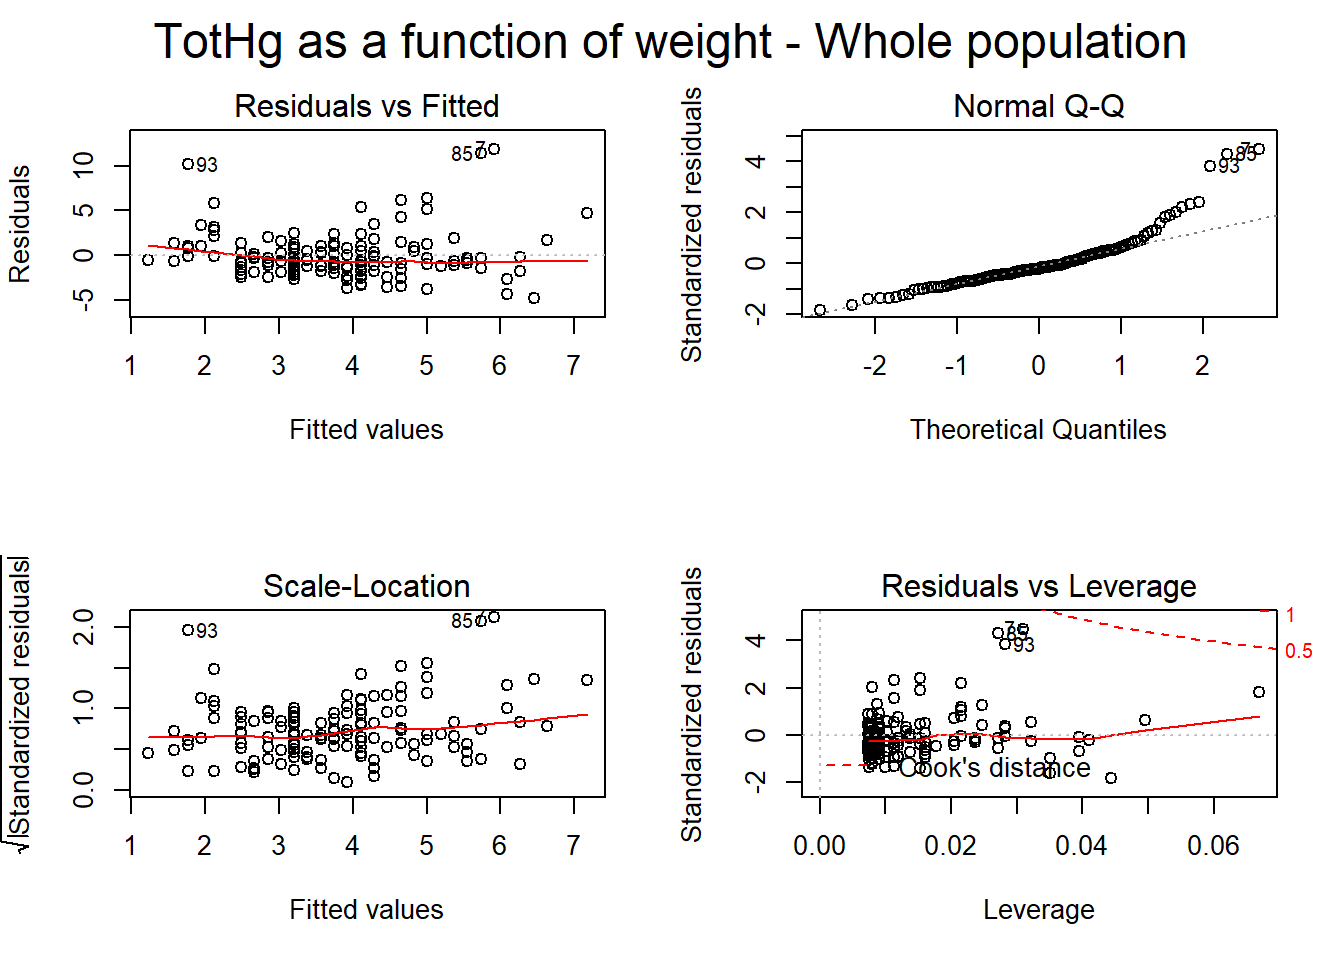
\includegraphics{Data_analysis_files/figure-latex/unnamed-chunk-13-1.pdf}

\begin{Shaded}
\begin{Highlighting}[]
\KeywordTok{par}\NormalTok{(}\DataTypeTok{mfrow=}\KeywordTok{c}\NormalTok{(}\DecValTok{2}\NormalTok{,}\DecValTok{2}\NormalTok{))}
\KeywordTok{plot}\NormalTok{(hg.lmFi.weight)}
\KeywordTok{mtext}\NormalTok{(}\StringTok{"TotHg as a function of weight - Fishermen population"}\NormalTok{, }\DataTypeTok{side =} \DecValTok{3}\NormalTok{, }\DataTypeTok{line =} \OperatorTok{-}\DecValTok{2}\NormalTok{, }\DataTypeTok{outer =} \OtherTok{TRUE}\NormalTok{, }\DataTypeTok{cex =} \FloatTok{1.5}\NormalTok{)}
\end{Highlighting}
\end{Shaded}

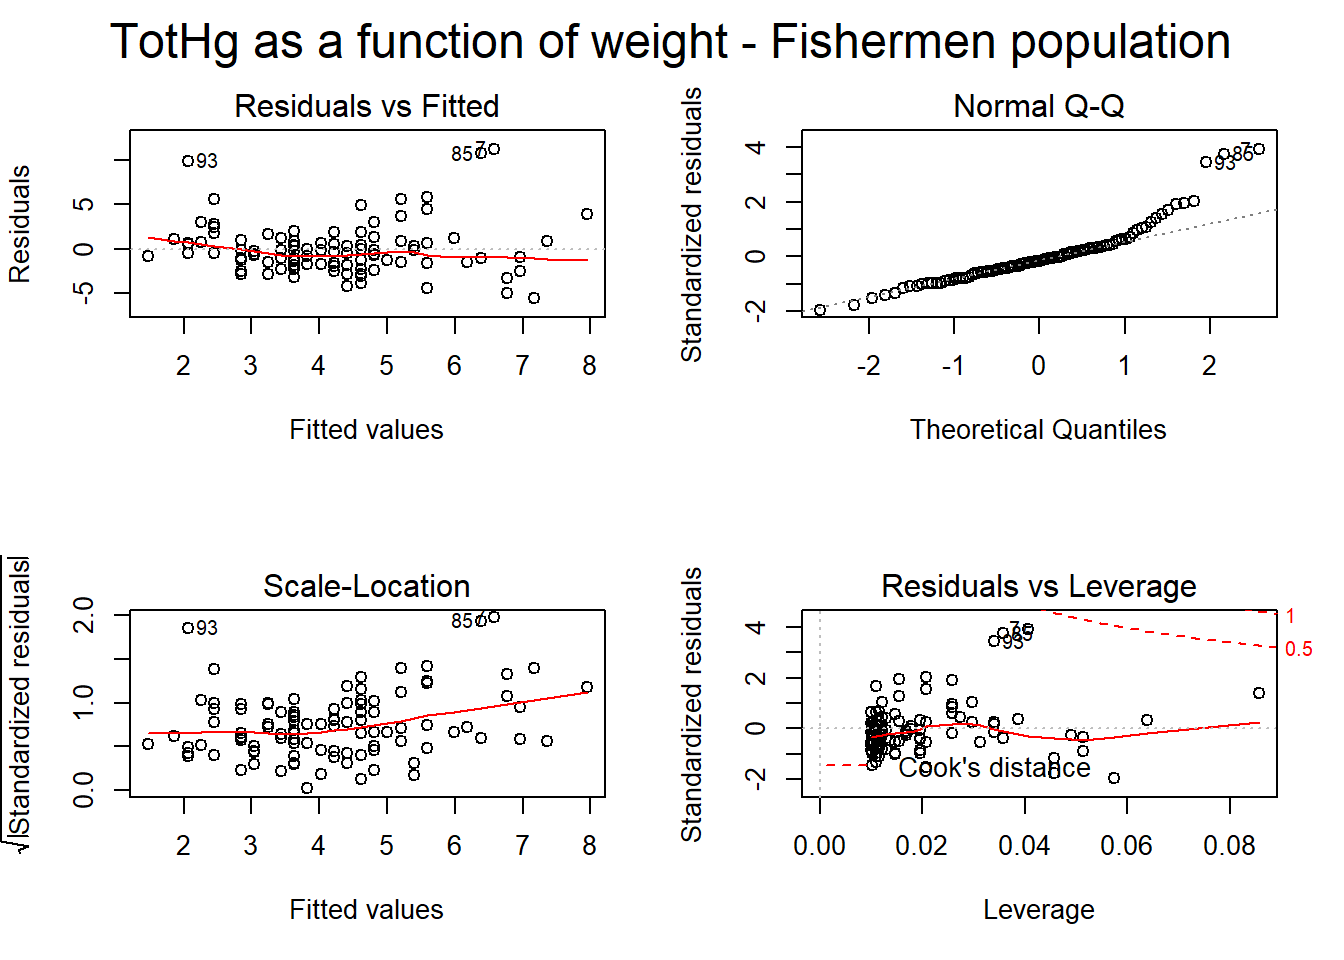
\includegraphics{Data_analysis_files/figure-latex/unnamed-chunk-13-2.pdf}

\begin{Shaded}
\begin{Highlighting}[]
\KeywordTok{par}\NormalTok{(}\DataTypeTok{mfrow=}\KeywordTok{c}\NormalTok{(}\DecValTok{2}\NormalTok{,}\DecValTok{2}\NormalTok{))}
\KeywordTok{plot}\NormalTok{(hg.lmNF.weight)}
\KeywordTok{mtext}\NormalTok{(}\StringTok{"TotHg as a function of weight - Non-Fishermen population"}\NormalTok{, }\DataTypeTok{side =} \DecValTok{3}\NormalTok{, }\DataTypeTok{line =} \OperatorTok{-}\DecValTok{2}\NormalTok{, }\DataTypeTok{outer =} \OtherTok{TRUE}\NormalTok{, }\DataTypeTok{cex =} \FloatTok{1.5}\NormalTok{)}
\end{Highlighting}
\end{Shaded}

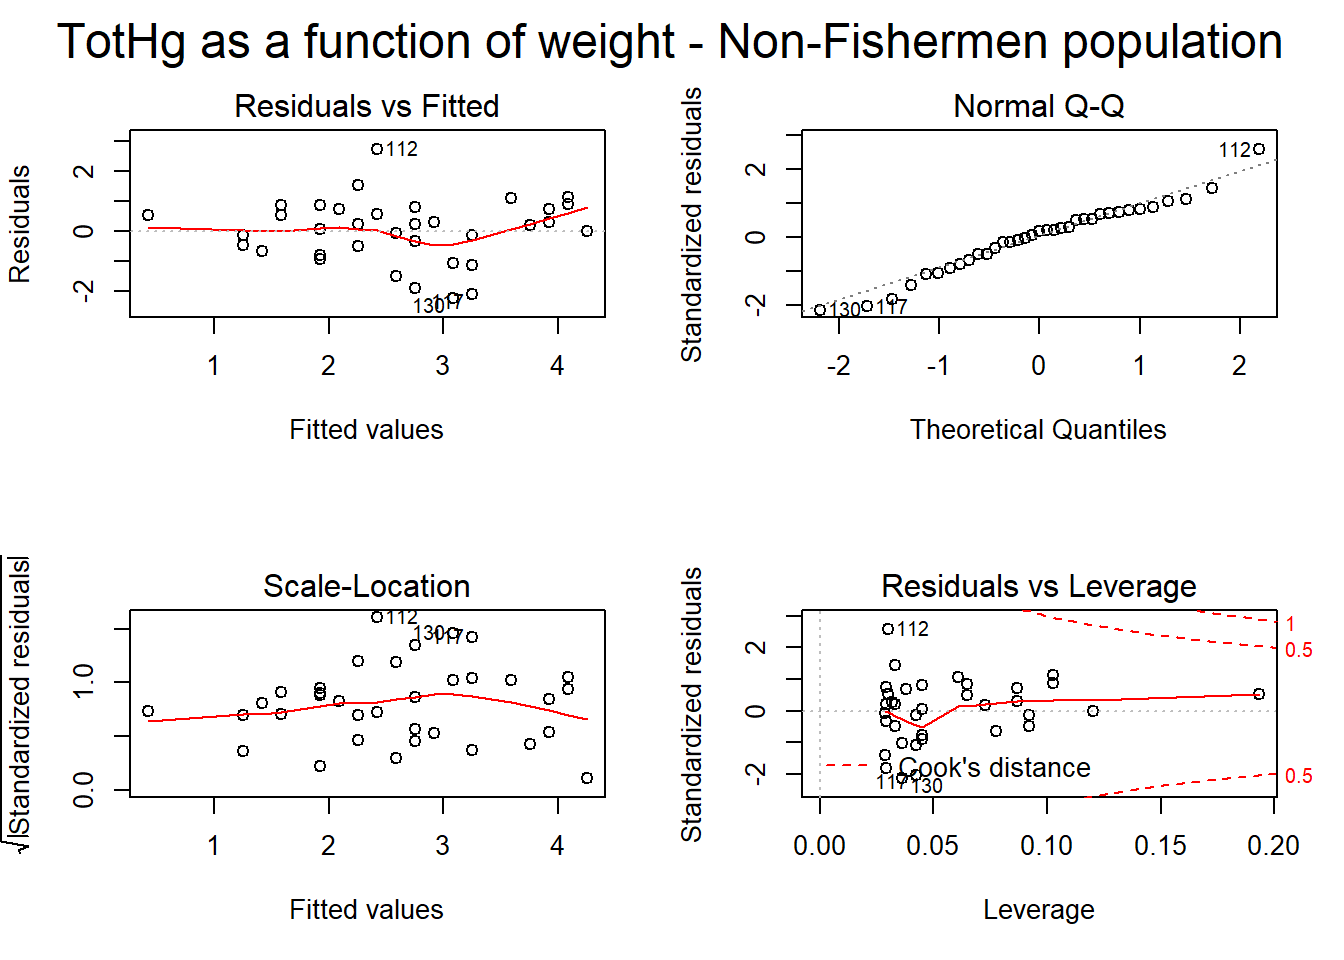
\includegraphics{Data_analysis_files/figure-latex/unnamed-chunk-13-3.pdf}
\#\#\#\#\# Comments

\paragraph{Height}\label{height}

\subparagraph{Code}\label{code-3}

\begin{Shaded}
\begin{Highlighting}[]
\NormalTok{hg.form.height =}\StringTok{ }\NormalTok{TotHg }\OperatorTok{~}\StringTok{ }\NormalTok{height}

\NormalTok{hg.lm.height =}\StringTok{ }\KeywordTok{lm}\NormalTok{(hg.form.height, }\DataTypeTok{data=}\NormalTok{dataset)}
\NormalTok{hg.lmFi.height =}\StringTok{ }\KeywordTok{lm}\NormalTok{(hg.form.height, }\DataTypeTok{data=}\NormalTok{dataset.fisherman)}
\NormalTok{hg.lmNF.height =}\StringTok{ }\KeywordTok{lm}\NormalTok{(hg.form.height, }\DataTypeTok{data=}\NormalTok{dataset.non_fisherman)}

\KeywordTok{par}\NormalTok{(}\DataTypeTok{mfrow=}\KeywordTok{c}\NormalTok{(}\DecValTok{2}\NormalTok{,}\DecValTok{2}\NormalTok{))}
\KeywordTok{plot}\NormalTok{(hg.lm.height)}
\KeywordTok{mtext}\NormalTok{(}\StringTok{"TotHg as a function of height - Whole population"}\NormalTok{, }\DataTypeTok{side =} \DecValTok{3}\NormalTok{, }\DataTypeTok{line =} \OperatorTok{-}\DecValTok{2}\NormalTok{, }\DataTypeTok{outer =} \OtherTok{TRUE}\NormalTok{, }\DataTypeTok{cex =} \FloatTok{1.5}\NormalTok{)}
\end{Highlighting}
\end{Shaded}

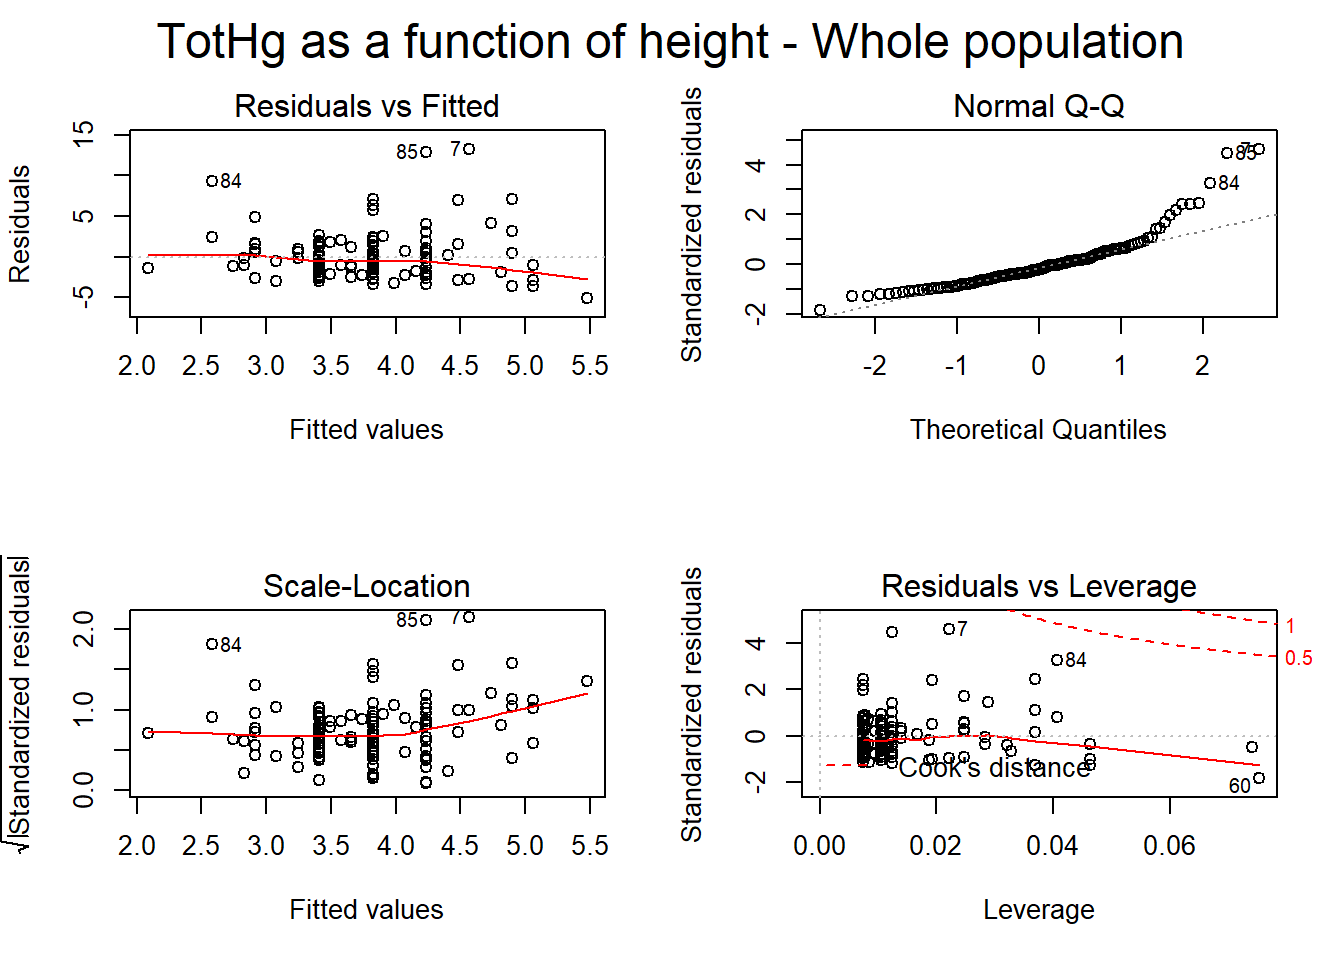
\includegraphics{Data_analysis_files/figure-latex/unnamed-chunk-14-1.pdf}

\begin{Shaded}
\begin{Highlighting}[]
\KeywordTok{par}\NormalTok{(}\DataTypeTok{mfrow=}\KeywordTok{c}\NormalTok{(}\DecValTok{2}\NormalTok{,}\DecValTok{2}\NormalTok{))}
\KeywordTok{plot}\NormalTok{(hg.lmFi.height)}
\KeywordTok{mtext}\NormalTok{(}\StringTok{"TotHg as a function of height - Fishermen population"}\NormalTok{, }\DataTypeTok{side =} \DecValTok{3}\NormalTok{, }\DataTypeTok{line =} \OperatorTok{-}\DecValTok{2}\NormalTok{, }\DataTypeTok{outer =} \OtherTok{TRUE}\NormalTok{, }\DataTypeTok{cex =} \FloatTok{1.5}\NormalTok{)}
\end{Highlighting}
\end{Shaded}

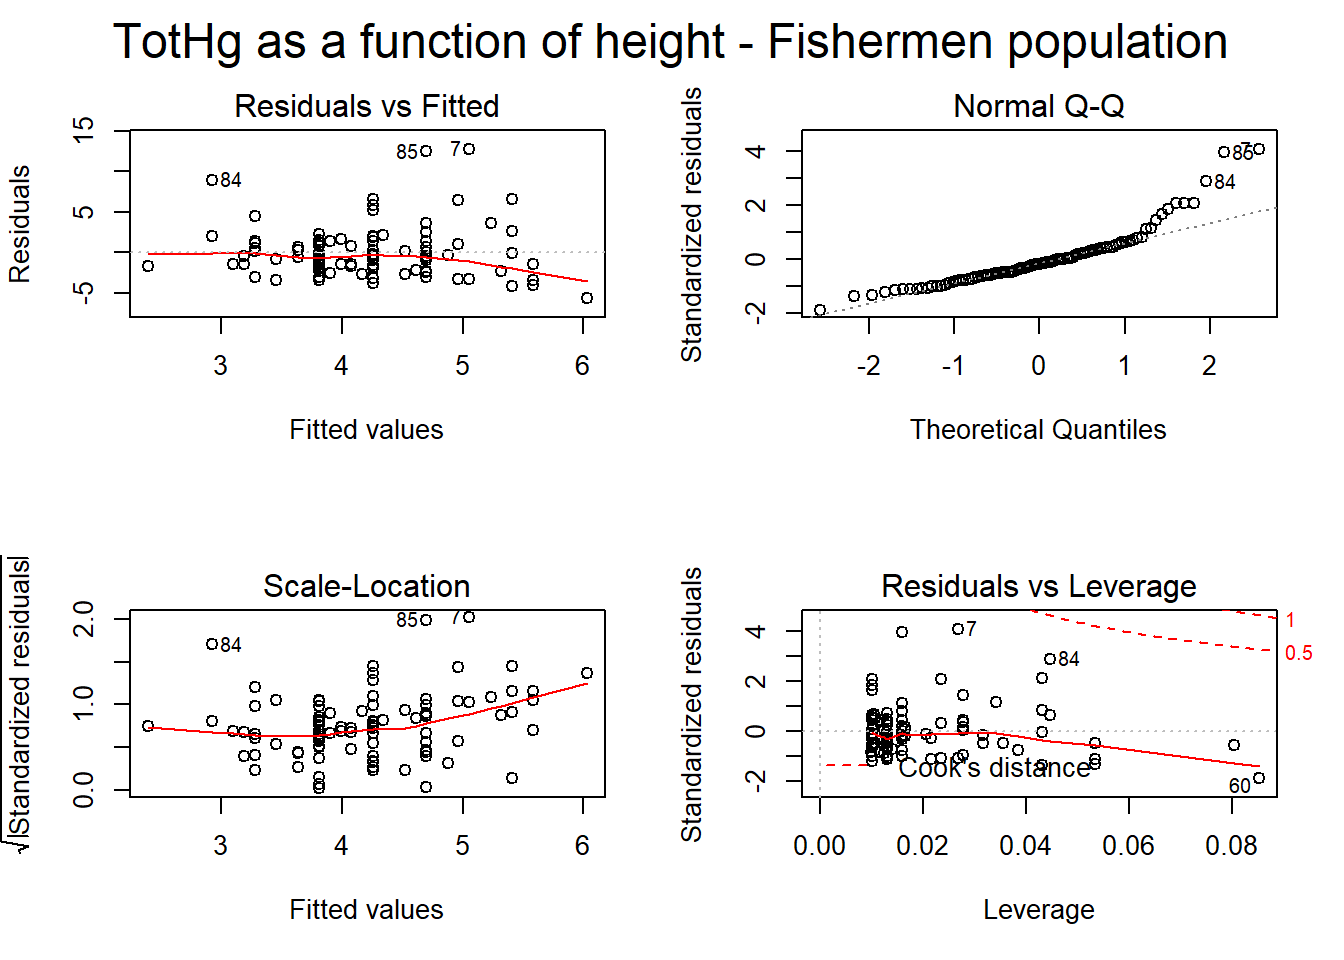
\includegraphics{Data_analysis_files/figure-latex/unnamed-chunk-14-2.pdf}

\begin{Shaded}
\begin{Highlighting}[]
\KeywordTok{par}\NormalTok{(}\DataTypeTok{mfrow=}\KeywordTok{c}\NormalTok{(}\DecValTok{2}\NormalTok{,}\DecValTok{2}\NormalTok{))}
\KeywordTok{plot}\NormalTok{(hg.lmNF.height)}
\KeywordTok{mtext}\NormalTok{(}\StringTok{"TotHg as a function of height - Non-Fishermen population"}\NormalTok{, }\DataTypeTok{side =} \DecValTok{3}\NormalTok{, }\DataTypeTok{line =} \OperatorTok{-}\DecValTok{2}\NormalTok{, }\DataTypeTok{outer =} \OtherTok{TRUE}\NormalTok{, }\DataTypeTok{cex =} \FloatTok{1.5}\NormalTok{)}
\end{Highlighting}
\end{Shaded}

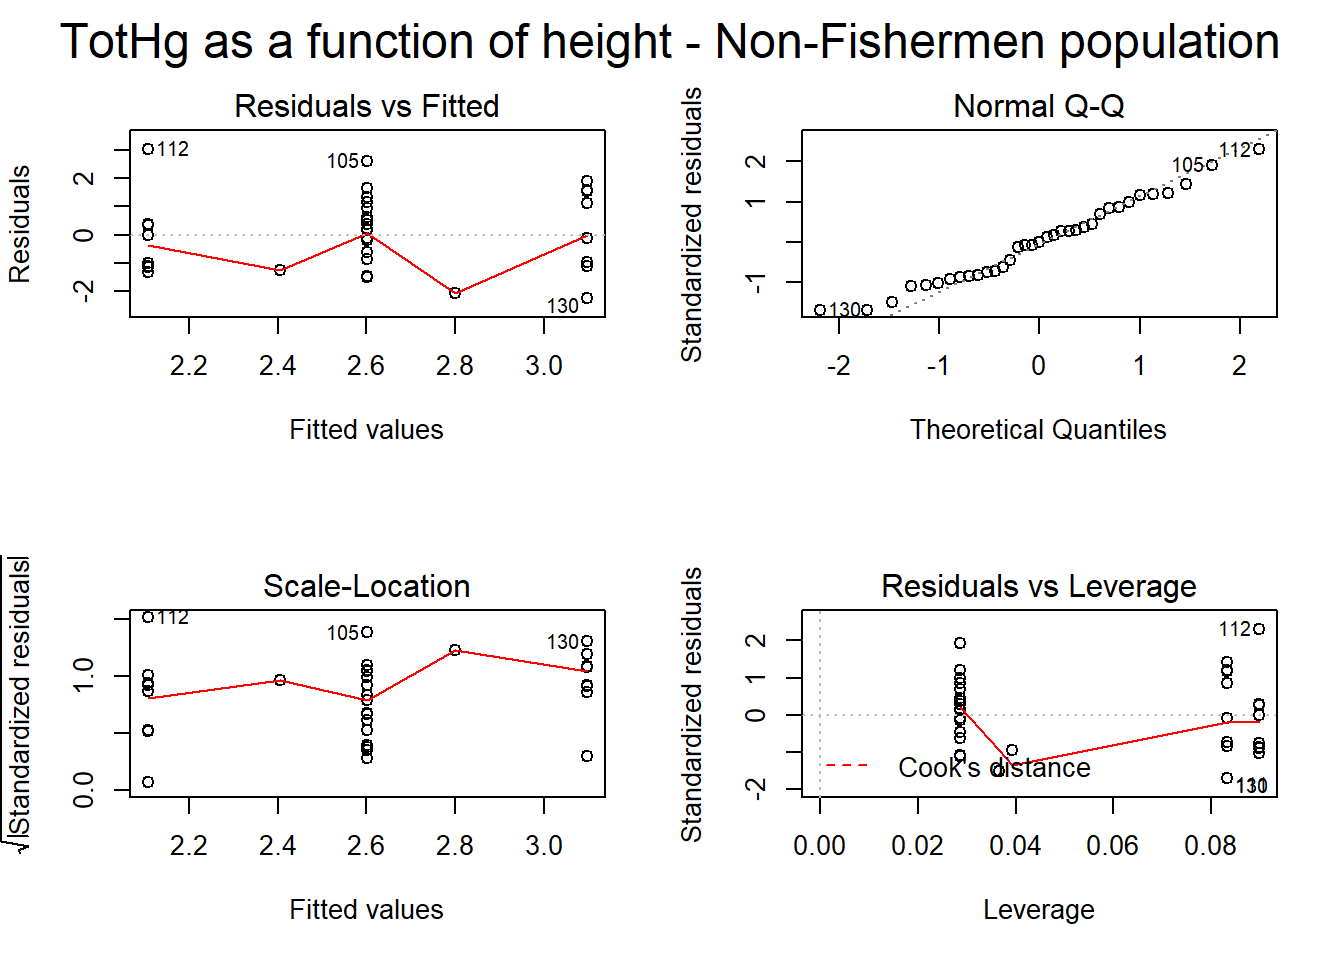
\includegraphics{Data_analysis_files/figure-latex/unnamed-chunk-14-3.pdf}

\subparagraph{Comments}\label{comments-2}

\paragraph{Fish meal per week}\label{fish-meal-per-week}

\subparagraph{Code}\label{code-4}

\begin{Shaded}
\begin{Highlighting}[]
\NormalTok{hg.form.fishmlwk =}\StringTok{ }\NormalTok{TotHg }\OperatorTok{~}\StringTok{ }\NormalTok{fishmlwk}

\NormalTok{hg.lm.fishmlwk =}\StringTok{ }\KeywordTok{lm}\NormalTok{(hg.form.fishmlwk, }\DataTypeTok{data=}\NormalTok{dataset)}
\NormalTok{hg.lmFi.fishmlwk =}\StringTok{ }\KeywordTok{lm}\NormalTok{(hg.form.fishmlwk, }\DataTypeTok{data=}\NormalTok{dataset.fisherman)}
\NormalTok{hg.lmNF.fishmlwk =}\StringTok{ }\KeywordTok{lm}\NormalTok{(hg.form.fishmlwk, }\DataTypeTok{data=}\NormalTok{dataset.non_fisherman)}

\KeywordTok{par}\NormalTok{(}\DataTypeTok{mfrow=}\KeywordTok{c}\NormalTok{(}\DecValTok{2}\NormalTok{,}\DecValTok{2}\NormalTok{))}
\KeywordTok{plot}\NormalTok{(hg.lm.fishmlwk)}
\KeywordTok{mtext}\NormalTok{(}\StringTok{"TotHg as a function of fishmlwk - Whole population"}\NormalTok{, }\DataTypeTok{side =} \DecValTok{3}\NormalTok{, }\DataTypeTok{line =} \OperatorTok{-}\DecValTok{2}\NormalTok{, }\DataTypeTok{outer =} \OtherTok{TRUE}\NormalTok{, }\DataTypeTok{cex =} \FloatTok{1.5}\NormalTok{)}
\end{Highlighting}
\end{Shaded}

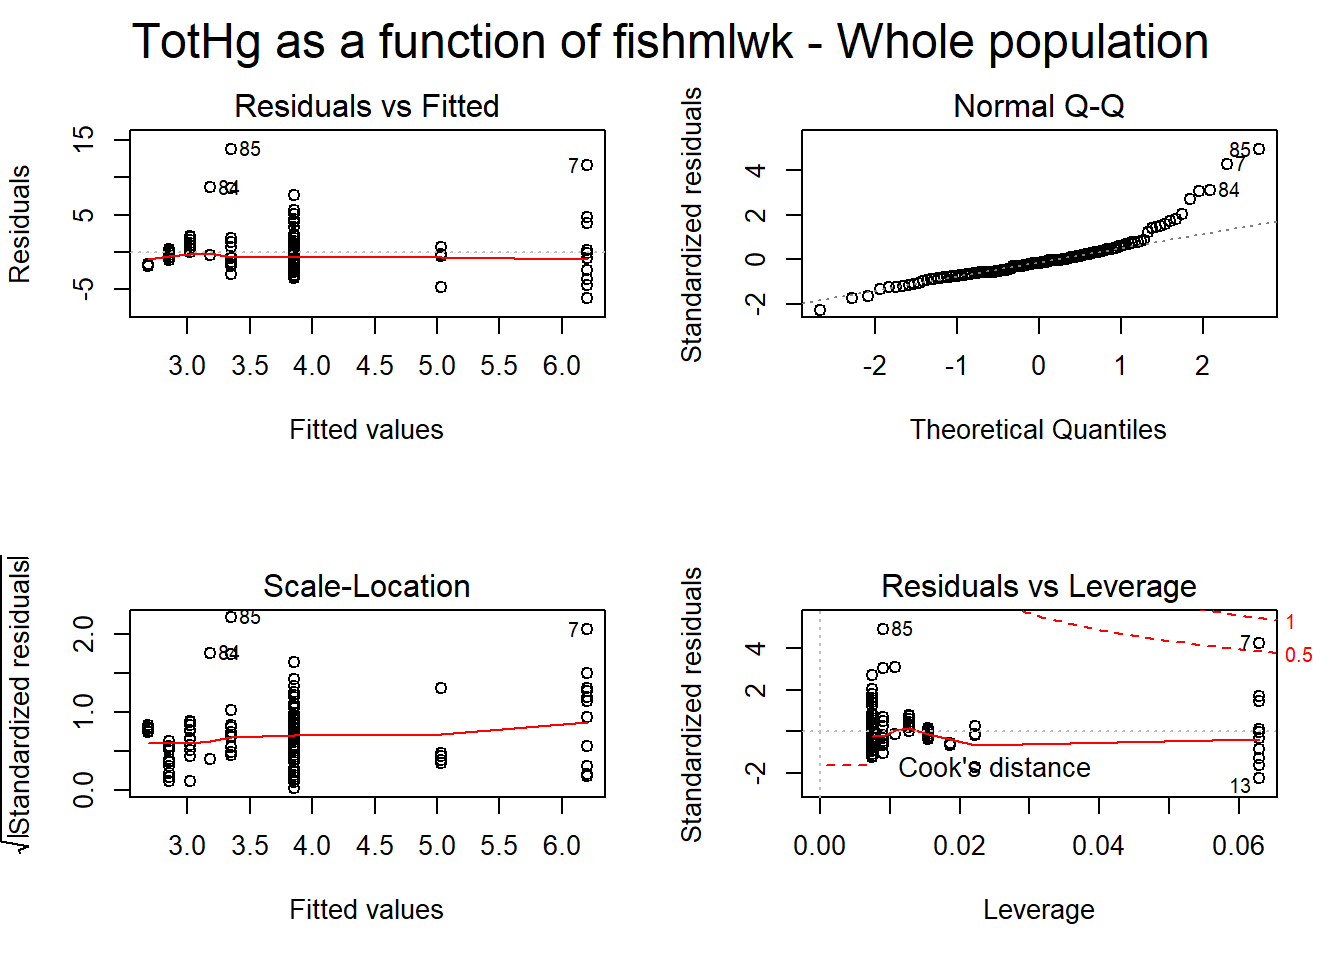
\includegraphics{Data_analysis_files/figure-latex/unnamed-chunk-15-1.pdf}

\begin{Shaded}
\begin{Highlighting}[]
\KeywordTok{par}\NormalTok{(}\DataTypeTok{mfrow=}\KeywordTok{c}\NormalTok{(}\DecValTok{2}\NormalTok{,}\DecValTok{2}\NormalTok{))}
\KeywordTok{plot}\NormalTok{(hg.lmFi.fishmlwk)}
\KeywordTok{mtext}\NormalTok{(}\StringTok{"TotHg as a function of fishmlwk - Fishermen population"}\NormalTok{, }\DataTypeTok{side =} \DecValTok{3}\NormalTok{, }\DataTypeTok{line =} \OperatorTok{-}\DecValTok{2}\NormalTok{, }\DataTypeTok{outer =} \OtherTok{TRUE}\NormalTok{, }\DataTypeTok{cex =} \FloatTok{1.5}\NormalTok{)}
\end{Highlighting}
\end{Shaded}

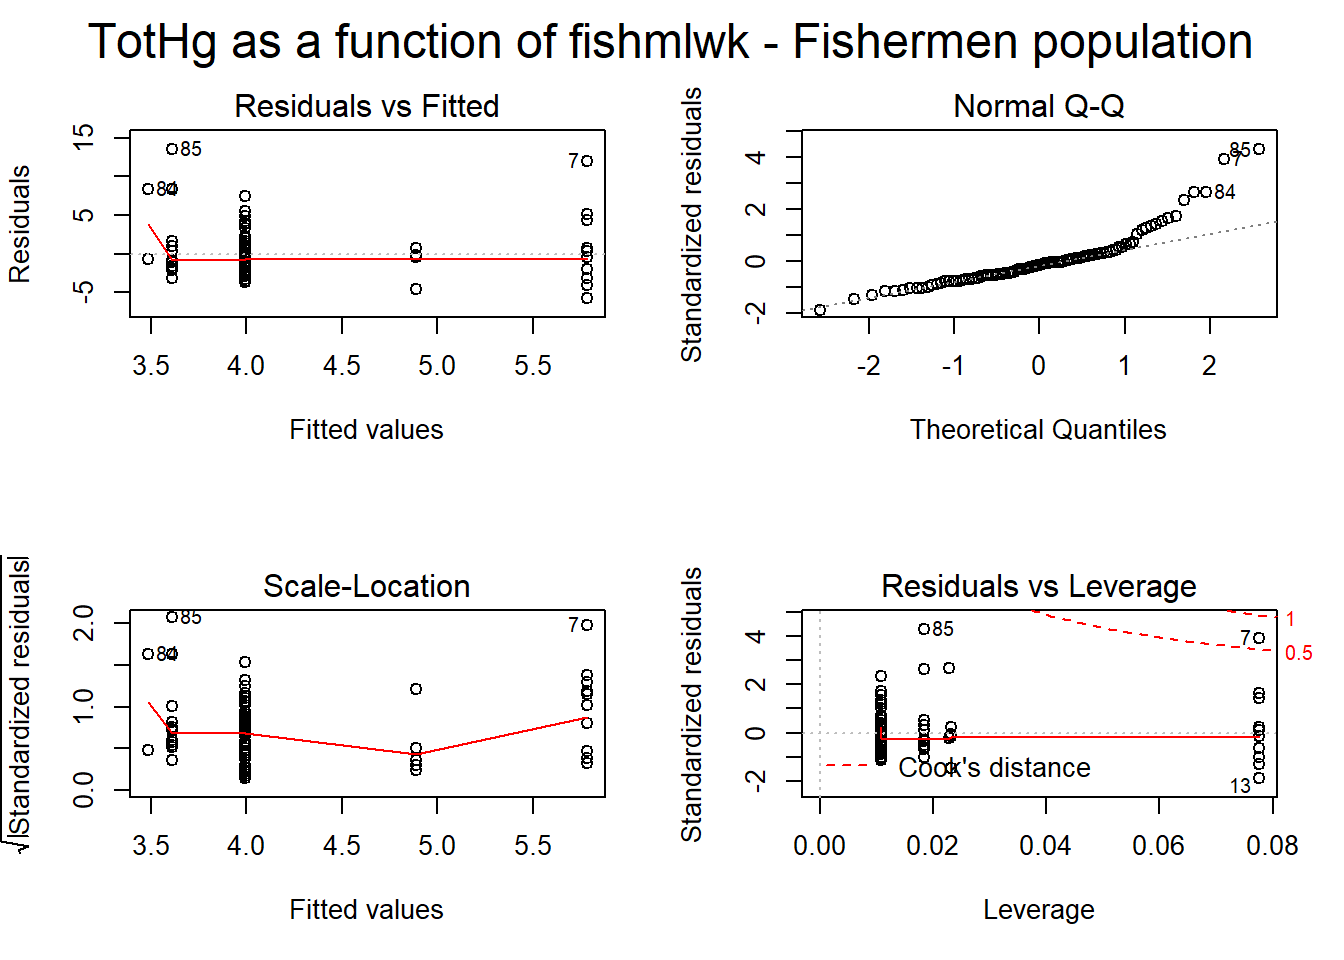
\includegraphics{Data_analysis_files/figure-latex/unnamed-chunk-15-2.pdf}

\begin{Shaded}
\begin{Highlighting}[]
\KeywordTok{par}\NormalTok{(}\DataTypeTok{mfrow=}\KeywordTok{c}\NormalTok{(}\DecValTok{2}\NormalTok{,}\DecValTok{2}\NormalTok{))}
\KeywordTok{plot}\NormalTok{(hg.lmNF.fishmlwk)}
\KeywordTok{mtext}\NormalTok{(}\StringTok{"TotHg as a function of fishmlwk - Non-Fishermen population"}\NormalTok{, }\DataTypeTok{side =} \DecValTok{3}\NormalTok{, }\DataTypeTok{line =} \OperatorTok{-}\DecValTok{2}\NormalTok{, }\DataTypeTok{outer =} \OtherTok{TRUE}\NormalTok{, }\DataTypeTok{cex =} \FloatTok{1.5}\NormalTok{)}
\end{Highlighting}
\end{Shaded}

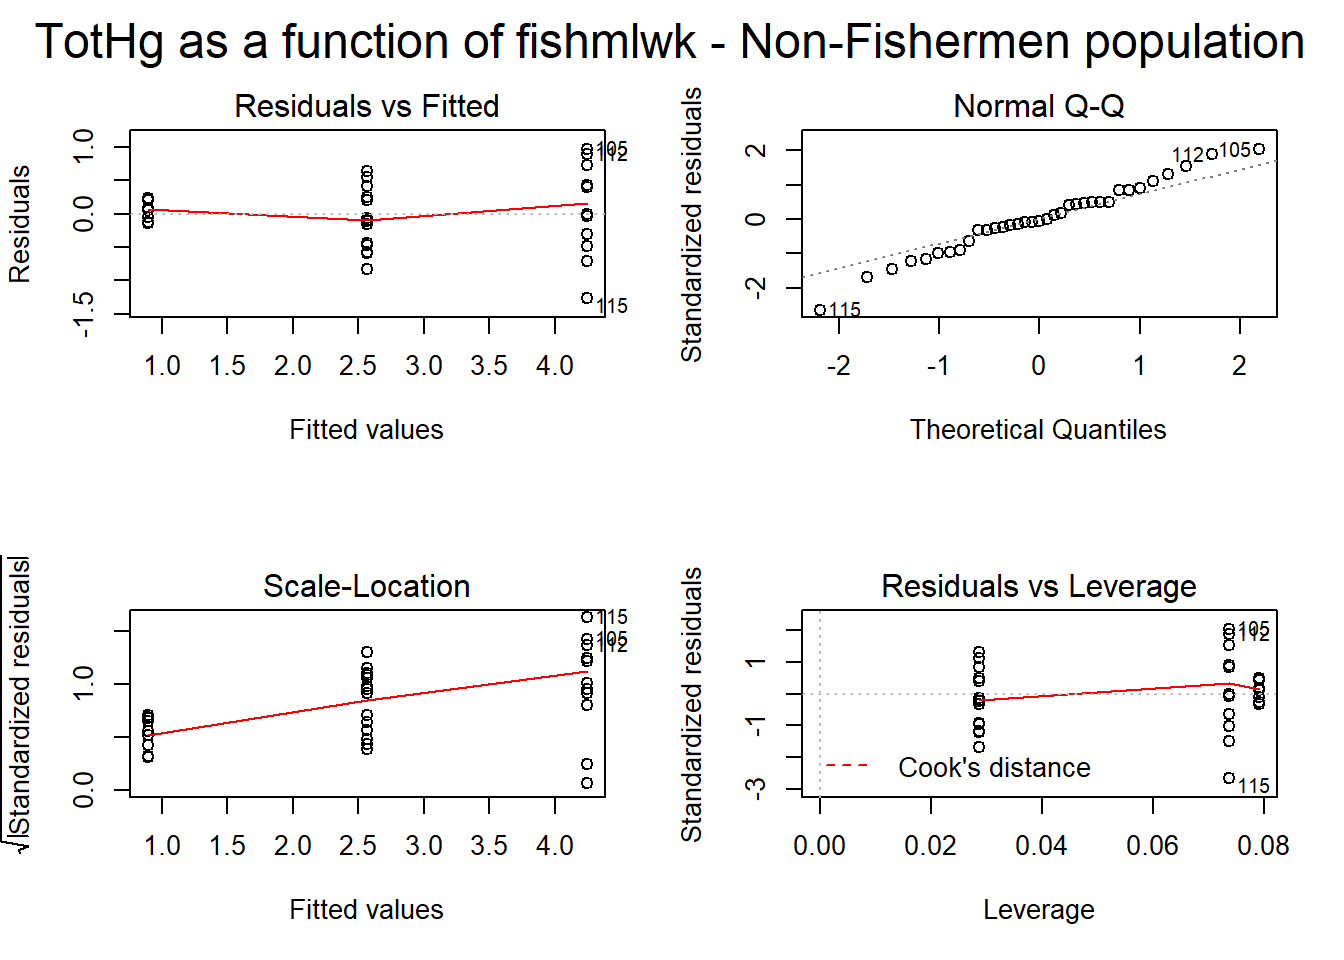
\includegraphics{Data_analysis_files/figure-latex/unnamed-chunk-15-3.pdf}

\subparagraph{Comments}\label{comments-3}

\subsubsection{Two groups significantly
different}\label{two-groups-significantly-different}

The fishermen have higher levels of mercury in their hair.

Test of the difference between fishermen and non-fishermen

\begin{Shaded}
\begin{Highlighting}[]
\NormalTok{hg.form.fisherman =}\StringTok{ }\NormalTok{TotHg }\OperatorTok{~}\StringTok{ }\NormalTok{fisherman}
\NormalTok{hg.aov.fisherman =}\StringTok{ }\KeywordTok{aov}\NormalTok{(hg.form.fisherman, }\DataTypeTok{data=}\NormalTok{ dataset)}
\KeywordTok{summary}\NormalTok{(hg.aov.fisherman)}
\end{Highlighting}
\end{Shaded}

\begin{verbatim}
##              Df Sum Sq Mean Sq F value  Pr(>F)   
## fisherman     1   63.4   63.43   7.714 0.00627 **
## Residuals   133 1093.7    8.22                   
## ---
## Signif. codes:  0 '***' 0.001 '**' 0.01 '*' 0.05 '.' 0.1 ' ' 1
\end{verbatim}

There is indeed a significant difference between these two groups. What
are the differences between the two populations that can explain such
observations?

Comments:

\begin{itemize}
\item
  The population of non-fishermen is between 25 and 35 years while the
  population of fishermen is between 15 and 60 years. As there seem to
  be a little correlation between age and mercury levels this could
  affect our other results.
\item
  The variable restime seems difficult to interpret (poor correlation
  with Hg levels, narrow range of values for non-fishermen).
\item
  The height indicator for non-fishermen is not very precise (it takes
  only 3 different values: 170cm, 175cm, 180cm).
\item
  There seems to be a correlation between weight and mercury levels.
  Should we study mercury levels per kg instead? (that may be not very
  relevant because the mercury levels are the mercury levels in the hair
  so there have no reason to be linearly correlated with the total mass
  of the body)
\item
  There is a clear difference in way of life between fishermen and
  non-fishermen: the first ones eat fish more often than the second. We
  have to be very careful in interpreting our results because any
  correlation found between high levels of fish consumption and mercury
  can reflect the correlation between being a fisherman and having high
  levels of mercury without meaning that it is fish consumption that
  causes high levels of Hg. However, among the non-fishermen population
  there seems to be a clear trend between fish consumption and Hg
  mercury.
\item
  No clear trend between fishpart and Hg levels, maybe we need to put in
  relation fishpart and fish consumption.
\item
  Unbalanced design (more fishermen than controls)
\end{itemize}

\begin{Shaded}
\begin{Highlighting}[]
\NormalTok{hg.form.fishpart =}\StringTok{ }\NormalTok{TotHg }\OperatorTok{~}\StringTok{ }\NormalTok{fishpart}
\NormalTok{hg.aov.fishpart =}\StringTok{ }\KeywordTok{aov}\NormalTok{(hg.form.fishpart, }\DataTypeTok{data=}\NormalTok{ dataset)}
\KeywordTok{summary}\NormalTok{(hg.aov.fishpart)}
\end{Highlighting}
\end{Shaded}

\begin{verbatim}
##              Df Sum Sq Mean Sq F value   Pr(>F)    
## fishpart      3  149.1   49.71   6.461 0.000411 ***
## Residuals   131 1007.9    7.69                     
## ---
## Signif. codes:  0 '***' 0.001 '**' 0.01 '*' 0.05 '.' 0.1 ' ' 1
\end{verbatim}

\subsection{Possible analysis}\label{possible-analysis}

\begin{itemize}
\item
  Add a correlation coefficient to the scatterplots
\item
  Check homoscedasticity
\item
  Fit a linear model to the data
\item
  Model selection:
\item
  Compare models using F-tests, AIC, BIC
\item
  If the number of variables is small enough, could compare all possible
  models. Usually this is not practical, use automatic procedures:
  forward selection, backward elimination, stepwise selection
\item
  Adjusted \(R^2\), ANOVA
\item
  Look for influential points (studentized residuals, Cook's distance)
\item
  Other diagnostic plots: residuals against predicted values, normal
  QQ-plot, scale location, residual vs leverage
\end{itemize}

\subsection{Plan}\label{plan}

\begin{itemize}
\item
  VIF to check for multicolinearity between variables + choose which we
  want to keep
\item
  stepwise selection on the model with interactions
\item
  fit the model, with the whole population, the fishermen, and the non
  fishermen
\item
  diagnostic plots
\item
  eventually robust regression
\item
  conclude for the values of the parameters + some nice plots
\end{itemize}

\subsubsection{Selection of the model}\label{selection-of-the-model}

\begin{Shaded}
\begin{Highlighting}[]
\NormalTok{hg.form.full =}\StringTok{ }\NormalTok{TotHg}\OperatorTok{~}\StringTok{ }\NormalTok{age }\OperatorTok{+}\StringTok{ }\NormalTok{restime }\OperatorTok{+}\StringTok{ }\NormalTok{height }\OperatorTok{+}\StringTok{ }\NormalTok{weight }\OperatorTok{+}\StringTok{ }\NormalTok{fishmlwk }\OperatorTok{+}\StringTok{ }\NormalTok{fishpart }
\NormalTok{hg.form.full2 =}\StringTok{ }\NormalTok{TotHg}\OperatorTok{~}\StringTok{ }\NormalTok{(age }\OperatorTok{+}\StringTok{ }\NormalTok{restime }\OperatorTok{+}\StringTok{ }\NormalTok{height }\OperatorTok{+}\StringTok{ }\NormalTok{weight }\OperatorTok{+}\StringTok{ }\NormalTok{fishmlwk }\OperatorTok{+}\StringTok{ }\NormalTok{fishpart)}\OperatorTok{^}\DecValTok{2}

\KeywordTok{vif}\NormalTok{(}\KeywordTok{lm}\NormalTok{(hg.form.full,}\DataTypeTok{data=}\NormalTok{dataset))}
\end{Highlighting}
\end{Shaded}

\begin{verbatim}
##              GVIF Df GVIF^(1/(2*Df))
## age      1.606389  1        1.267434
## restime  1.562206  1        1.249882
## height   1.137883  1        1.066716
## weight   1.188214  1        1.090052
## fishmlwk 1.211887  1        1.100857
## fishpart 1.368546  3        1.053683
\end{verbatim}

\begin{itemize}
\tightlist
\item
  The Variance Inflation Factors tends to show there is no case of too
  high colinearity here. (BUT problem with the fact we have categorical
  var vs.~continuous var ?)
\end{itemize}

\paragraph{Whole population, non-squared
model}\label{whole-population-non-squared-model}

\begin{Shaded}
\begin{Highlighting}[]
\NormalTok{fit <-}\StringTok{ }\KeywordTok{lm}\NormalTok{(hg.form.full,}\DataTypeTok{data=}\NormalTok{dataset)}
\NormalTok{step <-}\StringTok{ }\KeywordTok{stepAIC}\NormalTok{(fit, }\DataTypeTok{direction=}\StringTok{"both"}\NormalTok{)}
\end{Highlighting}
\end{Shaded}

\begin{verbatim}
## Start:  AIC=260.18
## TotHg ~ age + restime + height + weight + fishmlwk + fishpart
## 
##            Df Sum of Sq    RSS    AIC
## - height    1     4.793 816.53 258.97
## - age       1     8.814 820.55 259.63
## - fishpart  3    33.660 845.39 259.66
## - restime   1    10.460 822.19 259.90
## <none>                  811.73 260.18
## - fishmlwk  1    46.822 858.55 265.75
## - weight    1   115.001 926.73 276.06
## 
## Step:  AIC=258.97
## TotHg ~ age + restime + weight + fishmlwk + fishpart
## 
##            Df Sum of Sq    RSS    AIC
## - age       1     9.289 825.81 258.50
## - fishpart  3    36.427 852.95 258.86
## <none>                  816.53 258.97
## - restime   1    12.200 828.73 258.97
## + height    1     4.793 811.73 260.18
## - fishmlwk  1    45.206 861.73 264.25
## - weight    1   139.057 955.58 278.20
## 
## Step:  AIC=258.5
## TotHg ~ restime + weight + fishmlwk + fishpart
## 
##            Df Sum of Sq    RSS    AIC
## - restime   1     4.799 830.61 257.28
## <none>                  825.81 258.50
## + age       1     9.289 816.53 258.97
## - fishpart  3    40.857 866.67 259.02
## + height    1     5.267 820.55 259.63
## - fishmlwk  1    52.912 878.73 264.88
## - weight    1   135.101 960.92 276.95
## 
## Step:  AIC=257.28
## TotHg ~ weight + fishmlwk + fishpart
## 
##            Df Sum of Sq    RSS    AIC
## - fishpart  3    37.460 868.07 257.24
## <none>                  830.61 257.28
## + height    1     6.330 824.28 258.25
## + restime   1     4.799 825.81 258.50
## + age       1     1.888 828.73 258.97
## - fishmlwk  1    49.571 880.19 263.11
## - weight    1   133.220 963.83 275.36
## 
## Step:  AIC=257.24
## TotHg ~ weight + fishmlwk
## 
##            Df Sum of Sq     RSS    AIC
## <none>                   868.07 257.24
## + fishpart  3    37.460  830.61 257.28
## + height    1     9.170  858.90 257.80
## + age       1     5.744  862.33 258.34
## + restime   1     1.402  866.67 259.02
## - fishmlwk  1    95.208  963.28 269.29
## - weight    1   182.853 1050.93 281.04
\end{verbatim}

\begin{Shaded}
\begin{Highlighting}[]
\NormalTok{step}\OperatorTok{$}\NormalTok{anova }\CommentTok{# display results}
\end{Highlighting}
\end{Shaded}

\begin{verbatim}
## Stepwise Model Path 
## Analysis of Deviance Table
## 
## Initial Model:
## TotHg ~ age + restime + height + weight + fishmlwk + fishpart
## 
## Final Model:
## TotHg ~ weight + fishmlwk
## 
## 
##         Step Df  Deviance Resid. Df Resid. Dev      AIC
## 1                               126   811.7328 260.1760
## 2   - height  1  4.793058       127   816.5259 258.9708
## 3      - age  1  9.288674       128   825.8146 258.4979
## 4  - restime  1  4.799172       129   830.6137 257.2802
## 5 - fishpart  3 37.459773       132   868.0735 257.2352
\end{verbatim}

\begin{Shaded}
\begin{Highlighting}[]
\KeywordTok{summary}\NormalTok{(step)}
\end{Highlighting}
\end{Shaded}

\begin{verbatim}
## 
## Call:
## lm(formula = TotHg ~ weight + fishmlwk, data = dataset)
## 
## Residuals:
##     Min      1Q  Median      3Q     Max 
## -4.8344 -1.3096 -0.2953  0.6279 11.8572 
## 
## Coefficients:
##              Estimate Std. Error t value Pr(>|t|)    
## (Intercept) -10.07682    2.44481  -4.122 6.60e-05 ***
## weight        0.17518    0.03322   5.273 5.34e-07 ***
## fishmlwk      0.15884    0.04175   3.805 0.000216 ***
## ---
## Signif. codes:  0 '***' 0.001 '**' 0.01 '*' 0.05 '.' 0.1 ' ' 1
## 
## Residual standard error: 2.564 on 132 degrees of freedom
## Multiple R-squared:  0.2498, Adjusted R-squared:  0.2384 
## F-statistic: 21.97 on 2 and 132 DF,  p-value: 5.787e-09
\end{verbatim}

\begin{Shaded}
\begin{Highlighting}[]
\KeywordTok{plot}\NormalTok{(step)}
\end{Highlighting}
\end{Shaded}

\includegraphics{Data_analysis_files/figure-latex/unnamed-chunk-19-1.pdf}
\includegraphics{Data_analysis_files/figure-latex/unnamed-chunk-19-2.pdf}
\includegraphics{Data_analysis_files/figure-latex/unnamed-chunk-19-3.pdf}
\includegraphics{Data_analysis_files/figure-latex/unnamed-chunk-19-4.pdf}
With this method of stewise selection, it seems that the best model
would be : TotHg \textasciitilde{} weight + fishmlwk The Multiple
R-squared is only 0.2498: it seems we are unable to explain most of the
variability of TotHg between individuals. However as the p-values for
those two parameters are excellents, their influence on TotHg seems well
established.

\paragraph{Attempt of backward
selection}\label{attempt-of-backward-selection}

\begin{Shaded}
\begin{Highlighting}[]
\NormalTok{hg.form.custom =}\StringTok{ }\NormalTok{TotHg }\OperatorTok{~}\StringTok{ }\NormalTok{age }\OperatorTok{+}\StringTok{ }\NormalTok{restime }\OperatorTok{+}\StringTok{ }\NormalTok{height }\OperatorTok{+}\StringTok{ }\NormalTok{weight }\OperatorTok{+}\StringTok{ }\NormalTok{fishmlwk }\OperatorTok{+}\StringTok{ }\NormalTok{fishpart}
\KeywordTok{drop1}\NormalTok{(}\KeywordTok{lm}\NormalTok{(hg.form.custom, }\DataTypeTok{data =}\NormalTok{ dataset), }\DataTypeTok{test=}\StringTok{"F"}\NormalTok{)}
\end{Highlighting}
\end{Shaded}

\begin{verbatim}
## Single term deletions
## 
## Model:
## TotHg ~ age + restime + height + weight + fishmlwk + fishpart
##          Df Sum of Sq    RSS    AIC F value    Pr(>F)    
## <none>                811.73 260.18                      
## age       1     8.814 820.55 259.63  1.3682   0.24433    
## restime   1    10.460 822.19 259.90  1.6236   0.20494    
## height    1     4.793 816.53 258.97  0.7440   0.39002    
## weight    1   115.001 926.73 276.06 17.8508 4.545e-05 ***
## fishmlwk  1    46.822 858.55 265.75  7.2678   0.00798 ** 
## fishpart  3    33.660 845.39 259.66  1.7416   0.16186    
## ---
## Signif. codes:  0 '***' 0.001 '**' 0.01 '*' 0.05 '.' 0.1 ' ' 1
\end{verbatim}

\begin{Shaded}
\begin{Highlighting}[]
\CommentTok{# > delete age}

\NormalTok{hg.form.custom =}\StringTok{ }\NormalTok{TotHg }\OperatorTok{~}\StringTok{ }\NormalTok{restime }\OperatorTok{+}\StringTok{ }\NormalTok{height }\OperatorTok{+}\StringTok{ }\NormalTok{weight }\OperatorTok{+}\StringTok{ }\NormalTok{fishmlwk }\OperatorTok{+}\StringTok{ }\NormalTok{fishpart}
\KeywordTok{drop1}\NormalTok{(}\KeywordTok{lm}\NormalTok{(hg.form.custom, }\DataTypeTok{data =}\NormalTok{ dataset), }\DataTypeTok{test=}\StringTok{"F"}\NormalTok{)}
\end{Highlighting}
\end{Shaded}

\begin{verbatim}
## Single term deletions
## 
## Model:
## TotHg ~ restime + height + weight + fishmlwk + fishpart
##          Df Sum of Sq    RSS    AIC F value    Pr(>F)    
## <none>                820.55 259.63                      
## restime   1     3.737 824.28 258.25  0.5784  0.448352    
## height    1     5.267 825.81 258.50  0.8153  0.368277    
## weight    1   111.119 931.67 274.78 17.1984 6.115e-05 ***
## fishmlwk  1    54.606 875.15 266.33  8.4516  0.004305 ** 
## fishpart  3    37.469 858.02 259.66  1.9331  0.127544    
## ---
## Signif. codes:  0 '***' 0.001 '**' 0.01 '*' 0.05 '.' 0.1 ' ' 1
\end{verbatim}

\begin{Shaded}
\begin{Highlighting}[]
\CommentTok{# > delete height}

\NormalTok{hg.form.custom =}\StringTok{ }\NormalTok{TotHg }\OperatorTok{~}\StringTok{ }\NormalTok{restime }\OperatorTok{+}\StringTok{ }\NormalTok{weight }\OperatorTok{+}\StringTok{ }\NormalTok{fishmlwk }\OperatorTok{+}\StringTok{ }\NormalTok{fishpart}
\KeywordTok{drop1}\NormalTok{(}\KeywordTok{lm}\NormalTok{(hg.form.custom, }\DataTypeTok{data =}\NormalTok{ dataset), }\DataTypeTok{test=}\StringTok{"F"}\NormalTok{)}
\end{Highlighting}
\end{Shaded}

\begin{verbatim}
## Single term deletions
## 
## Model:
## TotHg ~ restime + weight + fishmlwk + fishpart
##          Df Sum of Sq    RSS    AIC F value    Pr(>F)    
## <none>                825.81 258.50                      
## restime   1     4.799 830.61 257.28  0.7439  0.390039    
## weight    1   135.101 960.92 276.95 20.9404 1.106e-05 ***
## fishmlwk  1    52.912 878.73 264.88  8.2013  0.004893 ** 
## fishpart  3    40.857 866.67 259.02  2.1109  0.102047    
## ---
## Signif. codes:  0 '***' 0.001 '**' 0.01 '*' 0.05 '.' 0.1 ' ' 1
\end{verbatim}

\begin{Shaded}
\begin{Highlighting}[]
\CommentTok{# > delete fishpart}

\NormalTok{hg.form.custom =}\StringTok{ }\NormalTok{TotHg }\OperatorTok{~}\StringTok{ }\NormalTok{restime }\OperatorTok{+}\StringTok{ }\NormalTok{weight }\OperatorTok{+}\StringTok{ }\NormalTok{fishmlwk}
\KeywordTok{drop1}\NormalTok{(}\KeywordTok{lm}\NormalTok{(hg.form.custom, }\DataTypeTok{data =}\NormalTok{ dataset), }\DataTypeTok{test=}\StringTok{"F"}\NormalTok{)}
\end{Highlighting}
\end{Shaded}

\begin{verbatim}
## Single term deletions
## 
## Model:
## TotHg ~ restime + weight + fishmlwk
##          Df Sum of Sq     RSS    AIC F value    Pr(>F)    
## <none>                 866.67 259.02                      
## restime   1     1.402  868.07 257.24  0.2119 0.6460703    
## weight    1   184.226 1050.90 283.04 27.8464 5.292e-07 ***
## fishmlwk  1    96.183  962.85 271.23 14.5383 0.0002105 ***
## ---
## Signif. codes:  0 '***' 0.001 '**' 0.01 '*' 0.05 '.' 0.1 ' ' 1
\end{verbatim}

\begin{Shaded}
\begin{Highlighting}[]
\CommentTok{# > delete restime}

\NormalTok{hg.form.custom =}\StringTok{ }\NormalTok{TotHg }\OperatorTok{~}\StringTok{ }\NormalTok{weight }\OperatorTok{+}\StringTok{ }\NormalTok{fishmlwk}
\KeywordTok{drop1}\NormalTok{(}\KeywordTok{lm}\NormalTok{(hg.form.custom, }\DataTypeTok{data =}\NormalTok{ dataset), }\DataTypeTok{test=}\StringTok{"F"}\NormalTok{)}
\end{Highlighting}
\end{Shaded}

\begin{verbatim}
## Single term deletions
## 
## Model:
## TotHg ~ weight + fishmlwk
##          Df Sum of Sq     RSS    AIC F value    Pr(>F)    
## <none>                 868.07 257.24                      
## weight    1   182.853 1050.93 281.04  27.805 5.337e-07 ***
## fishmlwk  1    95.208  963.28 269.29  14.477 0.0002161 ***
## ---
## Signif. codes:  0 '***' 0.001 '**' 0.01 '*' 0.05 '.' 0.1 ' ' 1
\end{verbatim}

\begin{Shaded}
\begin{Highlighting}[]
\KeywordTok{summary}\NormalTok{(}\KeywordTok{lm}\NormalTok{(hg.form.custom, }\DataTypeTok{data =}\NormalTok{ dataset))}
\end{Highlighting}
\end{Shaded}

\begin{verbatim}
## 
## Call:
## lm(formula = hg.form.custom, data = dataset)
## 
## Residuals:
##     Min      1Q  Median      3Q     Max 
## -4.8344 -1.3096 -0.2953  0.6279 11.8572 
## 
## Coefficients:
##              Estimate Std. Error t value Pr(>|t|)    
## (Intercept) -10.07682    2.44481  -4.122 6.60e-05 ***
## weight        0.17518    0.03322   5.273 5.34e-07 ***
## fishmlwk      0.15884    0.04175   3.805 0.000216 ***
## ---
## Signif. codes:  0 '***' 0.001 '**' 0.01 '*' 0.05 '.' 0.1 ' ' 1
## 
## Residual standard error: 2.564 on 132 degrees of freedom
## Multiple R-squared:  0.2498, Adjusted R-squared:  0.2384 
## F-statistic: 21.97 on 2 and 132 DF,  p-value: 5.787e-09
\end{verbatim}

\begin{Shaded}
\begin{Highlighting}[]
\CommentTok{# > seems ok !}
\CommentTok{# The backward selection gives the same model than stepwise.}
\end{Highlighting}
\end{Shaded}

\paragraph{Whole population, squared
model}\label{whole-population-squared-model}

\begin{Shaded}
\begin{Highlighting}[]
\NormalTok{fit <-}\StringTok{ }\KeywordTok{lm}\NormalTok{(hg.form.full2,}\DataTypeTok{data=}\NormalTok{dataset)}
\NormalTok{step <-}\StringTok{ }\KeywordTok{stepAIC}\NormalTok{(fit, }\DataTypeTok{direction=}\StringTok{"both"}\NormalTok{)}
\end{Highlighting}
\end{Shaded}

\begin{verbatim}
## Start:  AIC=243.9
## TotHg ~ (age + restime + height + weight + fishmlwk + fishpart)^2
## 
##                     Df Sum of Sq    RSS    AIC
## - restime:height     1     0.002 504.25 241.90
## - weight:fishmlwk    1     0.302 504.55 241.98
## - age:restime        1     1.880 506.13 242.41
## - fishmlwk:fishpart  2    12.231 516.48 243.14
## - height:weight      1     5.721 509.97 243.43
## - restime:weight     1     5.915 510.17 243.48
## <none>                           504.25 243.90
## - age:height         1    10.902 515.15 244.79
## - height:fishmlwk    1    14.327 518.58 245.69
## - age:fishmlwk       1    17.863 522.11 246.60
## - restime:fishmlwk   1    20.409 524.66 247.26
## - height:fishpart    3    46.197 550.45 249.74
## - age:weight         1    35.393 539.64 251.06
## - restime:fishpart   3    57.649 561.90 252.52
## - weight:fishpart    3    63.049 567.30 253.81
## - age:fishpart       3    67.828 572.08 254.94
## 
## Step:  AIC=241.9
## TotHg ~ age + restime + height + weight + fishmlwk + fishpart + 
##     age:restime + age:height + age:weight + age:fishmlwk + age:fishpart + 
##     restime:weight + restime:fishmlwk + restime:fishpart + height:weight + 
##     height:fishmlwk + height:fishpart + weight:fishmlwk + weight:fishpart + 
##     fishmlwk:fishpart
## 
##                     Df Sum of Sq    RSS    AIC
## - weight:fishmlwk    1     0.308 504.56 239.99
## - age:restime        1     1.878 506.13 240.41
## - fishmlwk:fishpart  2    12.343 516.60 241.17
## - height:weight      1     5.785 510.04 241.44
## - restime:weight     1     6.753 511.01 241.70
## <none>                           504.25 241.90
## - height:fishmlwk    1    14.416 518.67 243.71
## + restime:height     1     0.002 504.25 243.90
## - age:fishmlwk       1    18.098 522.35 244.66
## - age:height         1    18.414 522.67 244.75
## - restime:fishmlwk   1    20.424 524.68 245.26
## - height:fishpart    3    46.213 550.46 247.74
## - age:weight         1    36.417 540.67 249.32
## - restime:fishpart   3    59.700 563.95 251.01
## - weight:fishpart    3    63.170 567.42 251.84
## - age:fishpart       3    69.159 573.41 253.25
## 
## Step:  AIC=239.99
## TotHg ~ age + restime + height + weight + fishmlwk + fishpart + 
##     age:restime + age:height + age:weight + age:fishmlwk + age:fishpart + 
##     restime:weight + restime:fishmlwk + restime:fishpart + height:weight + 
##     height:fishmlwk + height:fishpart + weight:fishpart + fishmlwk:fishpart
## 
##                     Df Sum of Sq    RSS    AIC
## - age:restime        1     1.792 506.35 238.46
## - fishmlwk:fishpart  2    13.155 517.71 239.46
## - height:weight      1     5.594 510.15 239.47
## - restime:weight     1     6.777 511.34 239.79
## <none>                           504.56 239.99
## + weight:fishmlwk    1     0.308 504.25 241.90
## + restime:height     1     0.008 504.55 241.98
## - age:fishmlwk       1    18.736 523.30 242.91
## - age:height         1    18.862 523.42 242.94
## - restime:fishmlwk   1    20.165 524.73 243.28
## - height:fishpart    3    45.969 550.53 245.76
## - height:fishmlwk    1    36.522 541.08 247.42
## - age:weight         1    39.041 543.60 248.05
## - restime:fishpart   3    59.513 564.07 249.04
## - weight:fishpart    3    63.349 567.91 249.95
## - age:fishpart       3    69.355 573.92 251.37
## 
## Step:  AIC=238.46
## TotHg ~ age + restime + height + weight + fishmlwk + fishpart + 
##     age:height + age:weight + age:fishmlwk + age:fishpart + restime:weight + 
##     restime:fishmlwk + restime:fishpart + height:weight + height:fishmlwk + 
##     height:fishpart + weight:fishpart + fishmlwk:fishpart
## 
##                     Df Sum of Sq    RSS    AIC
## - fishmlwk:fishpart  2    11.612 517.96 237.53
## - height:weight      1     6.388 512.74 238.16
## - restime:weight     1     7.396 513.75 238.42
## <none>                           506.35 238.46
## + age:restime        1     1.792 504.56 239.99
## + weight:fishmlwk    1     0.222 506.13 240.41
## + restime:height     1     0.000 506.35 240.46
## - age:fishmlwk       1    17.148 523.50 240.96
## - age:height         1    17.858 524.21 241.14
## - restime:fishmlwk   1    18.534 524.89 241.32
## - height:fishpart    3    44.300 550.65 243.79
## - height:fishmlwk    1    36.641 542.99 245.90
## - age:weight         1    37.779 544.13 246.18
## - restime:fishpart   3    58.078 564.43 247.12
## - weight:fishpart    3    63.919 570.27 248.51
## - age:fishpart       3    67.694 574.05 249.40
## 
## Step:  AIC=237.53
## TotHg ~ age + restime + height + weight + fishmlwk + fishpart + 
##     age:height + age:weight + age:fishmlwk + age:fishpart + restime:weight + 
##     restime:fishmlwk + restime:fishpart + height:weight + height:fishmlwk + 
##     height:fishpart + weight:fishpart
## 
##                     Df Sum of Sq    RSS    AIC
## - height:weight      1     5.735 523.70 237.01
## <none>                           517.96 237.53
## - age:fishmlwk       1     8.142 526.11 237.63
## + fishmlwk:fishpart  2    11.612 506.35 238.46
## - age:height         1    13.483 531.45 238.99
## + weight:fishmlwk    1     1.040 516.92 239.25
## - restime:weight     1    15.250 533.21 239.44
## + age:restime        1     0.249 517.71 239.46
## + restime:height     1     0.144 517.82 239.49
## - restime:fishmlwk   1    19.252 537.22 240.45
## - height:fishpart    3    43.067 561.03 242.31
## - restime:fishpart   3    50.611 568.58 244.11
## - height:fishmlwk    1    39.744 557.71 245.51
## - weight:fishpart    3    66.997 584.96 247.95
## - age:weight         1    50.936 568.90 248.19
## - age:fishpart       3    84.404 602.37 251.91
## 
## Step:  AIC=237.01
## TotHg ~ age + restime + height + weight + fishmlwk + fishpart + 
##     age:height + age:weight + age:fishmlwk + age:fishpart + restime:weight + 
##     restime:fishmlwk + restime:fishpart + height:fishmlwk + height:fishpart + 
##     weight:fishpart
## 
##                     Df Sum of Sq    RSS    AIC
## <none>                           523.70 237.01
## - age:fishmlwk       1     9.067 532.77 237.33
## + height:weight      1     5.735 517.96 237.53
## + fishmlwk:fishpart  2    10.959 512.74 238.16
## - age:height         1    13.280 536.98 238.39
## + age:restime        1     0.585 523.11 238.86
## + weight:fishmlwk    1     0.580 523.12 238.86
## + restime:height     1     0.001 523.70 239.01
## - restime:fishmlwk   1    19.219 542.92 239.88
## - restime:weight     1    21.955 545.65 240.56
## - restime:fishpart   3    45.739 569.44 242.32
## - height:fishpart    3    50.550 574.25 243.45
## - height:fishmlwk    1    41.420 565.12 245.29
## - weight:fishpart    3    63.468 587.17 246.46
## - age:fishpart       3    79.611 603.31 250.12
## - age:weight         1    70.408 594.11 252.04
\end{verbatim}

\begin{Shaded}
\begin{Highlighting}[]
\NormalTok{step}\OperatorTok{$}\NormalTok{anova }\CommentTok{# display results}
\end{Highlighting}
\end{Shaded}

\begin{verbatim}
## Stepwise Model Path 
## Analysis of Deviance Table
## 
## Initial Model:
## TotHg ~ (age + restime + height + weight + fishmlwk + fishpart)^2
## 
## Final Model:
## TotHg ~ age + restime + height + weight + fishmlwk + fishpart + 
##     age:height + age:weight + age:fishmlwk + age:fishpart + restime:weight + 
##     restime:fishmlwk + restime:fishpart + height:fishmlwk + height:fishpart + 
##     weight:fishpart
## 
## 
##                  Step Df    Deviance Resid. Df Resid. Dev      AIC
## 1                                          102   504.2502 243.9027
## 2    - restime:height  1  0.00210511       103   504.2523 241.9033
## 3   - weight:fishmlwk  1  0.30810010       104   504.5604 239.9857
## 4       - age:restime  1  1.79187890       105   506.3522 238.4643
## 5 - fishmlwk:fishpart  2 11.61165927       107   517.9639 237.5252
## 6     - height:weight  1  5.73511231       108   523.6990 237.0117
\end{verbatim}

\begin{Shaded}
\begin{Highlighting}[]
\KeywordTok{summary}\NormalTok{(step)}
\end{Highlighting}
\end{Shaded}

\begin{verbatim}
## 
## Call:
## lm(formula = TotHg ~ age + restime + height + weight + fishmlwk + 
##     fishpart + age:height + age:weight + age:fishmlwk + age:fishpart + 
##     restime:weight + restime:fishmlwk + restime:fishpart + height:fishmlwk + 
##     height:fishpart + weight:fishpart, data = dataset)
## 
## Residuals:
##     Min      1Q  Median      3Q     Max 
## -4.9677 -1.1398 -0.1562  1.0264  6.1050 
## 
## Coefficients:
##                     Estimate Std. Error t value Pr(>|t|)    
## (Intercept)       19.9549895 53.1245877   0.376 0.707932    
## age               -0.2374601  0.9984923  -0.238 0.812472    
## restime            1.7362487  2.3850789   0.728 0.468212    
## height             0.1711573  0.3193397   0.536 0.593080    
## weight            -0.7075644  0.2917650  -2.425 0.016962 *  
## fishmlwk          -3.2102060  1.1976842  -2.680 0.008507 ** 
## fishpart1         14.7472272 49.5530215   0.298 0.766576    
## fishpart2         -9.0236684 46.4920822  -0.194 0.846470    
## fishpart3         10.5651405 51.3047913   0.206 0.837234    
## age:height        -0.0087869  0.0053097  -1.655 0.100850    
## age:weight         0.0250575  0.0065759   3.811 0.000231 ***
## age:fishmlwk      -0.0095060  0.0069516  -1.367 0.174323    
## age:fishpart1      0.2134939  0.3557009   0.600 0.549626    
## age:fishpart2      0.0000465  0.3361351   0.000 0.999890    
## age:fishpart3      0.5583238  0.3658675   1.526 0.129926    
## restime:weight    -0.0165245  0.0077659  -2.128 0.035625 *  
## restime:fishmlwk   0.0199387  0.0100153   1.991 0.049027 *  
## restime:fishpart1 -1.0401209  2.2903922  -0.454 0.650651    
## restime:fishpart2 -0.6501172  2.2882553  -0.284 0.776870    
## restime:fishpart3 -1.0158480  2.2933712  -0.443 0.658688    
## height:fishmlwk    0.0205744  0.0070396   2.923 0.004228 ** 
## height:fishpart1  -0.1289446  0.3065165  -0.421 0.674826    
## height:fishpart2   0.0636703  0.2885678   0.221 0.825787    
## height:fishpart3  -0.4762967  0.3385023  -1.407 0.162278    
## weight:fishpart1   0.0818027  0.2457439   0.333 0.739872    
## weight:fishpart2   0.0153310  0.2298895   0.067 0.946953    
## weight:fishpart3   0.8112189  0.3147254   2.578 0.011298 *  
## ---
## Signif. codes:  0 '***' 0.001 '**' 0.01 '*' 0.05 '.' 0.1 ' ' 1
## 
## Residual standard error: 2.202 on 108 degrees of freedom
## Multiple R-squared:  0.5474, Adjusted R-squared:  0.4384 
## F-statistic: 5.024 on 26 and 108 DF,  p-value: 1.109e-09
\end{verbatim}

\subsubsection{Fit of the selected
model}\label{fit-of-the-selected-model}

\paragraph{Code}\label{code-5}

\begin{Shaded}
\begin{Highlighting}[]
\NormalTok{selected.model =}\StringTok{ }\NormalTok{TotHg }\OperatorTok{~}\StringTok{ }\NormalTok{age }\OperatorTok{+}\StringTok{ }\NormalTok{restime }\OperatorTok{+}\StringTok{ }\NormalTok{height }\OperatorTok{+}\StringTok{ }\NormalTok{weight }\OperatorTok{+}\StringTok{ }\NormalTok{fishmlwk }\OperatorTok{+}\StringTok{ }\NormalTok{fishpart }\OperatorTok{+}\StringTok{ }\NormalTok{age}\OperatorTok{:}\NormalTok{height }\OperatorTok{+}\StringTok{ }\NormalTok{age}\OperatorTok{:}\NormalTok{weight }\OperatorTok{+}\StringTok{ }\NormalTok{age}\OperatorTok{:}\NormalTok{fishpart }\OperatorTok{+}\StringTok{ }\NormalTok{restime}\OperatorTok{:}\NormalTok{weight }\OperatorTok{+}\StringTok{ }\NormalTok{restime}\OperatorTok{:}\NormalTok{fishmlwk }\OperatorTok{+}\StringTok{ }\NormalTok{restime}\OperatorTok{:}\NormalTok{fishpart }\OperatorTok{+}\StringTok{ }\NormalTok{height}\OperatorTok{:}\NormalTok{fishmlwk }\OperatorTok{+}\StringTok{ }\NormalTok{height}\OperatorTok{:}\NormalTok{fishpart }\OperatorTok{+}\StringTok{ }\NormalTok{weight}\OperatorTok{:}\NormalTok{fishpart}

\NormalTok{hg.lm.selected.model=}\KeywordTok{lm}\NormalTok{(selected.model, }\DataTypeTok{data=}\NormalTok{dataset)}
\NormalTok{hg.lmFi.selected.model=}\KeywordTok{lm}\NormalTok{(selected.model, }\DataTypeTok{data=}\NormalTok{dataset.fisherman)}
\NormalTok{hg.lmNF.selected.model=}\KeywordTok{lm}\NormalTok{(selected.model, }\DataTypeTok{data=}\NormalTok{dataset.non_fisherman)}

\KeywordTok{summary}\NormalTok{(hg.lm.selected.model)}
\end{Highlighting}
\end{Shaded}

\begin{verbatim}
## 
## Call:
## lm(formula = selected.model, data = dataset)
## 
## Residuals:
##     Min      1Q  Median      3Q     Max 
## -4.7826 -1.0144 -0.2124  0.8760  6.1297 
## 
## Coefficients:
##                    Estimate Std. Error t value Pr(>|t|)    
## (Intercept)       24.981784  53.208315   0.470 0.639644    
## age               -0.412173   0.994228  -0.415 0.679274    
## restime            1.795995   2.394176   0.750 0.454779    
## height             0.140765   0.319834   0.440 0.660723    
## weight            -0.704960   0.292921  -2.407 0.017781 *  
## fishmlwk          -3.241359   1.202236  -2.696 0.008129 ** 
## fishpart1         12.627404  49.726018   0.254 0.800021    
## fishpart2         -7.524995  46.664268  -0.161 0.872189    
## fishpart3         10.527728  51.509107   0.204 0.838433    
## age:height        -0.007766   0.005278  -1.471 0.144063    
## age:weight         0.025053   0.006602   3.795 0.000243 ***
## age:fishpart1      0.067387   0.340625   0.198 0.843545    
## age:fishpart2     -0.068695   0.333678  -0.206 0.837275    
## age:fishpart3      0.468567   0.361365   1.297 0.197487    
## restime:weight    -0.017359   0.007773  -2.233 0.027571 *  
## restime:fishmlwk   0.012259   0.008325   1.472 0.143784    
## restime:fishpart1 -0.891040   2.296907  -0.388 0.698824    
## restime:fishpart2 -0.594226   2.297002  -0.259 0.796357    
## restime:fishpart3 -0.903354   2.301023  -0.393 0.695390    
## height:fishmlwk    0.019042   0.006978   2.729 0.007407 ** 
## height:fishpart1  -0.094828   0.306716  -0.309 0.757780    
## height:fishpart2   0.065931   0.289712   0.228 0.820405    
## height:fishpart3  -0.463851   0.339728  -1.365 0.174950    
## weight:fishpart1   0.085785   0.246705   0.348 0.728721    
## weight:fishpart2   0.018290   0.230795   0.079 0.936980    
## weight:fishpart3   0.819267   0.315924   2.593 0.010812 *  
## ---
## Signif. codes:  0 '***' 0.001 '**' 0.01 '*' 0.05 '.' 0.1 ' ' 1
## 
## Residual standard error: 2.211 on 109 degrees of freedom
## Multiple R-squared:  0.5396, Adjusted R-squared:  0.434 
## F-statistic: 5.109 on 25 and 109 DF,  p-value: 1.025e-09
\end{verbatim}

\begin{Shaded}
\begin{Highlighting}[]
\KeywordTok{summary}\NormalTok{(hg.lmFi.selected.model)}
\end{Highlighting}
\end{Shaded}

\begin{verbatim}
## 
## Call:
## lm(formula = selected.model, data = dataset.fisherman)
## 
## Residuals:
##     Min      1Q  Median      3Q     Max 
## -5.3642 -1.5448 -0.0712  1.4663  5.6957 
## 
## Coefficients:
##                     Estimate Std. Error t value Pr(>|t|)   
## (Intercept)        41.714299  46.590508   0.895  0.37333   
## age                -0.456802   1.130905  -0.404  0.68736   
## restime             0.843434   0.721336   1.169  0.24581   
## height             -0.003519   0.270079  -0.013  0.98964   
## weight             -0.545177   0.309911  -1.759  0.08243 . 
## fishmlwk           -2.916617   1.523614  -1.914  0.05921 . 
## fishpart2         -21.229382  20.833440  -1.019  0.31131   
## fishpart3          -1.770745  32.746970  -0.054  0.95701   
## age:height         -0.007250   0.006113  -1.186  0.23917   
## age:weight          0.025474   0.007897   3.226  0.00183 **
## age:fishpart2      -0.140504   0.095471  -1.472  0.14508   
## age:fishpart3       0.379636   0.186099   2.040  0.04470 * 
## restime:weight     -0.017988   0.009052  -1.987  0.05037 . 
## restime:fishmlwk    0.017535   0.010367   1.691  0.09469 . 
## restime:fishpart2   0.355986   0.156873   2.269  0.02598 * 
## restime:fishpart3   0.078375   0.219395   0.357  0.72187   
## height:fishmlwk     0.016742   0.008912   1.879  0.06399 . 
## height:fishpart2    0.204607   0.129904   1.575  0.11924   
## height:fishpart3   -0.333149   0.243637  -1.367  0.17538   
## weight:fishpart2   -0.161967   0.144947  -1.117  0.26720   
## weight:fishpart3    0.643322   0.293728   2.190  0.03146 * 
## ---
## Signif. codes:  0 '***' 0.001 '**' 0.01 '*' 0.05 '.' 0.1 ' ' 1
## 
## Residual standard error: 2.521 on 79 degrees of freedom
## Multiple R-squared:  0.5108, Adjusted R-squared:  0.3869 
## F-statistic: 4.124 on 20 and 79 DF,  p-value: 3.014e-06
\end{verbatim}

\begin{Shaded}
\begin{Highlighting}[]
\KeywordTok{summary}\NormalTok{(hg.lmNF.selected.model)}
\end{Highlighting}
\end{Shaded}

\begin{verbatim}
## 
## Call:
## lm(formula = selected.model, data = dataset.non_fisherman)
## 
## Residuals:
##      Min       1Q   Median       3Q      Max 
## -0.62234 -0.09610 -0.00379  0.08914  0.55459 
## 
## Coefficients:
##                     Estimate Std. Error t value Pr(>|t|)   
## (Intercept)        36.596286  80.012135   0.457  0.65441   
## age                -1.555857   2.604720  -0.597  0.55983   
## restime            -0.319986   4.142193  -0.077  0.93952   
## height             -0.424264   0.498117  -0.852  0.40869   
## weight              0.571077   0.250525   2.280  0.03883 * 
## fishmlwk          -24.011624  17.203224  -1.396  0.18453   
## fishpart1          95.745727  45.785381   2.091  0.05523 . 
## fishpart2          44.283630  29.031066   1.525  0.14943   
## age:height          0.016179   0.017723   0.913  0.37674   
## age:weight         -0.018116   0.009150  -1.980  0.06773 . 
## age:fishpart1       0.485522   0.135223   3.591  0.00295 **
## age:fishpart2      -0.001470   0.087674  -0.017  0.98686   
## restime:weight     -0.005438   0.055128  -0.099  0.92282   
## restime:fishmlwk    0.332154   0.732277   0.454  0.65708   
## restime:fishpart1  -1.104359   1.388306  -0.795  0.43962   
## restime:fishpart2   0.267880   0.916348   0.292  0.77432   
## height:fishmlwk     0.139328   0.104784   1.330  0.20489   
## height:fishpart1   -0.589596   0.273646  -2.155  0.04910 * 
## height:fishpart2   -0.278770   0.172470  -1.616  0.12832   
## weight:fishpart1   -0.047403   0.055493  -0.854  0.40736   
## weight:fishpart2    0.056973   0.053737   1.060  0.30700   
## ---
## Signif. codes:  0 '***' 0.001 '**' 0.01 '*' 0.05 '.' 0.1 ' ' 1
## 
## Residual standard error: 0.3245 on 14 degrees of freedom
## Multiple R-squared:  0.978,  Adjusted R-squared:  0.9466 
## F-statistic: 31.12 on 20 and 14 DF,  p-value: 2.396e-08
\end{verbatim}

\paragraph{Comments}\label{comments-4}

\subsubsection{Diagnostic plots}\label{diagnostic-plots}

\paragraph{Code}\label{code-6}

\begin{Shaded}
\begin{Highlighting}[]
\KeywordTok{plot}\NormalTok{(hg.lm.selected.model, }\DataTypeTok{which=}\DecValTok{1}\NormalTok{)}
\end{Highlighting}
\end{Shaded}

\includegraphics{Data_analysis_files/figure-latex/unnamed-chunk-23-1.pdf}

\begin{Shaded}
\begin{Highlighting}[]
\KeywordTok{plot}\NormalTok{(hg.lm.selected.model, }\DataTypeTok{which=}\DecValTok{2}\NormalTok{)}
\end{Highlighting}
\end{Shaded}

\includegraphics{Data_analysis_files/figure-latex/unnamed-chunk-23-2.pdf}

\begin{Shaded}
\begin{Highlighting}[]
\KeywordTok{plot}\NormalTok{(hg.lm.selected.model, }\DataTypeTok{which=}\DecValTok{3}\NormalTok{)}
\end{Highlighting}
\end{Shaded}

\includegraphics{Data_analysis_files/figure-latex/unnamed-chunk-23-3.pdf}

\begin{Shaded}
\begin{Highlighting}[]
\KeywordTok{plot}\NormalTok{(hg.lm.selected.model, }\DataTypeTok{which=}\DecValTok{4}\NormalTok{)}
\end{Highlighting}
\end{Shaded}

\includegraphics{Data_analysis_files/figure-latex/unnamed-chunk-23-4.pdf}

\begin{Shaded}
\begin{Highlighting}[]
\KeywordTok{plot}\NormalTok{(hg.lm.selected.model, }\DataTypeTok{which=}\DecValTok{5}\NormalTok{)}
\end{Highlighting}
\end{Shaded}

\includegraphics{Data_analysis_files/figure-latex/unnamed-chunk-23-5.pdf}

\begin{Shaded}
\begin{Highlighting}[]
\KeywordTok{plot}\NormalTok{(hg.lm.selected.model, }\DataTypeTok{which=}\DecValTok{6}\NormalTok{)}
\end{Highlighting}
\end{Shaded}

\includegraphics{Data_analysis_files/figure-latex/unnamed-chunk-23-6.pdf}

\paragraph{Comments}\label{comments-5}

It seems that there are some influencial points and we sould maybe
remove them to analyse the results without them.

\subsubsection{Removing the influencial
points}\label{removing-the-influencial-points}

\begin{Shaded}
\begin{Highlighting}[]
\NormalTok{dataset.without.inf=dataset[}\KeywordTok{c}\NormalTok{(}\OperatorTok{-}\DecValTok{6}\NormalTok{,}\OperatorTok{-}\DecValTok{56}\NormalTok{,}\OperatorTok{-}\DecValTok{70}\NormalTok{,}\OperatorTok{-}\DecValTok{85}\NormalTok{),]}
\NormalTok{dataset.fisherman.without.inf=dataset.fisherman[}\KeywordTok{c}\NormalTok{(}\OperatorTok{-}\DecValTok{6}\NormalTok{,}\OperatorTok{-}\DecValTok{56}\NormalTok{,}\OperatorTok{-}\DecValTok{70}\NormalTok{,}\OperatorTok{-}\DecValTok{85}\NormalTok{),]}
\NormalTok{dataset.non_fisherman.without.inf=dataset.non_fisherman[}\KeywordTok{c}\NormalTok{(}\OperatorTok{-}\DecValTok{6}\NormalTok{,}\OperatorTok{-}\DecValTok{56}\NormalTok{,}\OperatorTok{-}\DecValTok{70}\NormalTok{,}\OperatorTok{-}\DecValTok{85}\NormalTok{),]}
\end{Highlighting}
\end{Shaded}

\subsubsection{New fit}\label{new-fit}

\begin{Shaded}
\begin{Highlighting}[]
\NormalTok{hg.lm.new.selected.model=}\KeywordTok{lm}\NormalTok{(selected.model, }\DataTypeTok{data=}\NormalTok{dataset.without.inf)}
\NormalTok{hg.lmFi.new.selected.model=}\KeywordTok{lm}\NormalTok{(selected.model, }\DataTypeTok{data=}\NormalTok{dataset.fisherman.without.inf)}
\NormalTok{hg.lmNF.new.selected.model=}\KeywordTok{lm}\NormalTok{(selected.model, }\DataTypeTok{data=}\NormalTok{dataset.non_fisherman.without.inf)}

\KeywordTok{summary}\NormalTok{(hg.lm.new.selected.model)}
\end{Highlighting}
\end{Shaded}

\begin{verbatim}
## 
## Call:
## lm(formula = selected.model, data = dataset.without.inf)
## 
## Residuals:
##     Min      1Q  Median      3Q     Max 
## -4.6566 -1.0609 -0.1059  0.7876  6.9176 
## 
## Coefficients:
##                    Estimate Std. Error t value Pr(>|t|)    
## (Intercept)        2.661664  49.596348   0.054 0.957303    
## age                0.256819   0.954104   0.269 0.788325    
## restime            0.861760   2.208321   0.390 0.697155    
## height             0.195453   0.295391   0.662 0.509630    
## weight            -0.509945   0.273526  -1.864 0.065067 .  
## fishmlwk          -4.746572   1.188419  -3.994 0.000121 ***
## fishpart1         33.540025  45.927883   0.730 0.466848    
## fishpart2          7.675486  42.974327   0.179 0.858591    
## fishpart3         44.135629  78.246045   0.564 0.573915    
## age:height        -0.008736   0.004948  -1.766 0.080358 .  
## age:weight         0.017727   0.006355   2.790 0.006269 ** 
## age:fishpart1      0.323090   0.319042   1.013 0.313537    
## age:fishpart2     -0.054656   0.305984  -0.179 0.858576    
## age:fishpart3      0.577663   0.701373   0.824 0.412024    
## restime:weight    -0.007359   0.007576  -0.971 0.333617    
## restime:fishmlwk   0.003968   0.008192   0.484 0.629140    
## restime:fishpart1 -0.932007   2.106658  -0.442 0.659102    
## restime:fishpart2 -0.335415   2.107046  -0.159 0.873827    
## restime:fishpart3 -0.429848   2.121973  -0.203 0.839863    
## height:fishmlwk    0.028101   0.006921   4.060 9.46e-05 ***
## height:fishpart1  -0.255528   0.284106  -0.899 0.370491    
## height:fishpart2  -0.033702   0.266874  -0.126 0.899749    
## height:fishpart3  -0.759303   1.004839  -0.756 0.451553    
## weight:fishpart1   0.080102   0.226317   0.354 0.724097    
## weight:fishpart2   0.030988   0.211663   0.146 0.883883    
## weight:fishpart3   0.959723   1.296247   0.740 0.460718    
## ---
## Signif. codes:  0 '***' 0.001 '**' 0.01 '*' 0.05 '.' 0.1 ' ' 1
## 
## Residual standard error: 2.027 on 105 degrees of freedom
## Multiple R-squared:  0.5519, Adjusted R-squared:  0.4452 
## F-statistic: 5.173 on 25 and 105 DF,  p-value: 1.021e-09
\end{verbatim}

\begin{Shaded}
\begin{Highlighting}[]
\KeywordTok{summary}\NormalTok{(hg.lmFi.new.selected.model)}
\end{Highlighting}
\end{Shaded}

\begin{verbatim}
## 
## Call:
## lm(formula = selected.model, data = dataset.fisherman.without.inf)
## 
## Residuals:
##     Min      1Q  Median      3Q     Max 
## -5.2003 -1.3465  0.0311  1.1577  6.6744 
## 
## Coefficients:
##                     Estimate Std. Error t value Pr(>|t|)    
## (Intercept)        43.872355  43.336649   1.012 0.314620    
## age                 0.524010   1.112808   0.471 0.639086    
## restime            -0.171606   0.730707  -0.235 0.814966    
## height             -0.137731   0.251259  -0.548 0.585207    
## weight             -0.339437   0.291889  -1.163 0.248558    
## fishmlwk           -4.676130   1.529576  -3.057 0.003096 ** 
## fishpart2         -29.417772  19.330365  -1.522 0.132254    
## fishpart3           1.048212  74.634176   0.014 0.988832    
## age:height         -0.008473   0.005757  -1.472 0.145256    
## age:weight          0.018041   0.007607   2.372 0.020281 *  
## age:fishpart2      -0.386600   0.114424  -3.379 0.001158 ** 
## age:fishpart3       0.196775   0.729221   0.270 0.788022    
## restime:weight     -0.007513   0.008904  -0.844 0.401480    
## restime:fishmlwk    0.006829   0.010209   0.669 0.505615    
## restime:fishpart2   0.682339   0.174803   3.903 0.000205 ***
## restime:fishpart3   0.587924   0.324639   1.811 0.074144 .  
## height:fishmlwk     0.027426   0.008983   3.053 0.003131 ** 
## height:fishpart2    0.287966   0.121858   2.363 0.020714 *  
## height:fishpart3   -0.361388   1.099962  -0.329 0.743415    
## weight:fishpart2   -0.165095   0.133261  -1.239 0.219252    
## weight:fishpart3    0.688826   1.488082   0.463 0.644780    
## ---
## Signif. codes:  0 '***' 0.001 '**' 0.01 '*' 0.05 '.' 0.1 ' ' 1
## 
## Residual standard error: 2.316 on 75 degrees of freedom
## Multiple R-squared:  0.522,  Adjusted R-squared:  0.3945 
## F-statistic: 4.095 on 20 and 75 DF,  p-value: 4.24e-06
\end{verbatim}

\begin{Shaded}
\begin{Highlighting}[]
\KeywordTok{summary}\NormalTok{(hg.lmNF.new.selected.model)}
\end{Highlighting}
\end{Shaded}

\begin{verbatim}
## 
## Call:
## lm(formula = selected.model, data = dataset.non_fisherman.without.inf)
## 
## Residuals:
##      Min       1Q   Median       3Q      Max 
## -0.62736 -0.07481 -0.02919  0.06583  0.55047 
## 
## Coefficients:
##                     Estimate Std. Error t value Pr(>|t|)   
## (Intercept)        33.734918  82.126444   0.411  0.68793   
## age                -1.412222   2.680184  -0.527  0.60713   
## restime             0.298330   4.375769   0.068  0.94668   
## height             -0.421240   0.510383  -0.825  0.42407   
## weight              0.591213   0.259017   2.283  0.03993 * 
## fishmlwk          -23.097006  17.696314  -1.305  0.21446   
## fishpart1          91.163570  47.570751   1.916  0.07757 . 
## fishpart2          40.558609  30.429616   1.333  0.20547   
## age:height          0.015324   0.018218   0.841  0.41546   
## age:weight         -0.017776   0.009394  -1.892  0.08093 . 
## age:fishpart1       0.468472   0.141629   3.308  0.00566 **
## age:fishpart2      -0.020205   0.095457  -0.212  0.83565   
## restime:weight     -0.012227   0.057682  -0.212  0.83542   
## restime:fishmlwk    0.403277   0.760222   0.530  0.60473   
## restime:fishpart1  -1.331245   1.475208  -0.902  0.38325   
## restime:fishpart2   0.069161   0.999403   0.069  0.94588   
## height:fishmlwk     0.133199   0.107878   1.235  0.23879   
## height:fishpart1   -0.551152   0.288096  -1.913  0.07802 . 
## height:fishpart2   -0.245249   0.185915  -1.319  0.20989   
## weight:fishpart1   -0.062699   0.062673  -1.000  0.33537   
## weight:fishpart2    0.041797   0.060956   0.686  0.50495   
## ---
## Signif. codes:  0 '***' 0.001 '**' 0.01 '*' 0.05 '.' 0.1 ' ' 1
## 
## Residual standard error: 0.3325 on 13 degrees of freedom
## Multiple R-squared:  0.9778, Adjusted R-squared:  0.9436 
## F-statistic: 28.62 on 20 and 13 DF,  p-value: 1.148e-07
\end{verbatim}

\subsubsection{New diagnostic plots}\label{new-diagnostic-plots}

\begin{Shaded}
\begin{Highlighting}[]
\KeywordTok{plot}\NormalTok{(hg.lm.new.selected.model, }\DataTypeTok{which=}\DecValTok{1}\NormalTok{)}
\end{Highlighting}
\end{Shaded}

\includegraphics{Data_analysis_files/figure-latex/unnamed-chunk-26-1.pdf}

\begin{Shaded}
\begin{Highlighting}[]
\KeywordTok{plot}\NormalTok{(hg.lm.new.selected.model, }\DataTypeTok{which=}\DecValTok{2}\NormalTok{)}
\end{Highlighting}
\end{Shaded}

\includegraphics{Data_analysis_files/figure-latex/unnamed-chunk-26-2.pdf}

\begin{Shaded}
\begin{Highlighting}[]
\KeywordTok{plot}\NormalTok{(hg.lm.new.selected.model, }\DataTypeTok{which=}\DecValTok{3}\NormalTok{)}
\end{Highlighting}
\end{Shaded}

\includegraphics{Data_analysis_files/figure-latex/unnamed-chunk-26-3.pdf}

\begin{Shaded}
\begin{Highlighting}[]
\KeywordTok{plot}\NormalTok{(hg.lm.new.selected.model, }\DataTypeTok{which=}\DecValTok{4}\NormalTok{)}
\end{Highlighting}
\end{Shaded}

\includegraphics{Data_analysis_files/figure-latex/unnamed-chunk-26-4.pdf}

\begin{Shaded}
\begin{Highlighting}[]
\KeywordTok{plot}\NormalTok{(hg.lm.new.selected.model, }\DataTypeTok{which=}\DecValTok{5}\NormalTok{)}
\end{Highlighting}
\end{Shaded}

\begin{verbatim}
## Warning in sqrt(crit * p * (1 - hh)/hh): production de NaN

## Warning in sqrt(crit * p * (1 - hh)/hh): production de NaN
\end{verbatim}

\includegraphics{Data_analysis_files/figure-latex/unnamed-chunk-26-5.pdf}

\begin{Shaded}
\begin{Highlighting}[]
\KeywordTok{plot}\NormalTok{(hg.lm.new.selected.model, }\DataTypeTok{which=}\DecValTok{6}\NormalTok{)}
\end{Highlighting}
\end{Shaded}

\includegraphics{Data_analysis_files/figure-latex/unnamed-chunk-26-6.pdf}

We should maybe use the robust regression because we have now other
influencial points.

\subsubsection{Robust regression}\label{robust-regression}

\begin{Shaded}
\begin{Highlighting}[]
\NormalTok{hg.rlm.selected.model <-}\StringTok{ }\KeywordTok{rlm}\NormalTok{(selected.model, }\DataTypeTok{data=}\NormalTok{dataset)  }\CommentTok{# robust reg model}
\CommentTok{#hg.rlmFi.selected.model <- rlm(selected.model, data=dataset.fisherman)}
\CommentTok{#hg.rlmNF.selected.model <- rlm(selected.model, data=dataset.non_fisherman)}

\KeywordTok{summary}\NormalTok{(hg.rlm.selected.model)}
\end{Highlighting}
\end{Shaded}

\begin{verbatim}
## 
## Call: rlm(formula = selected.model, data = dataset)
## Residuals:
##      Min       1Q   Median       3Q      Max 
## -6.07936 -0.75778 -0.07816  0.84256  9.23039 
## 
## Coefficients:
##                   Value   Std. Error t value
## (Intercept)       20.4116 45.1313     0.4523
## age               -0.4640  0.8433    -0.5502
## restime            0.6663  2.0307     0.3281
## height             0.0164  0.2713     0.0603
## weight            -0.3164  0.2485    -1.2734
## fishmlwk          -3.9053  1.0197    -3.8297
## fishpart1         21.0513 42.1776     0.4991
## fishpart2          9.3541 39.5807     0.2363
## fishpart3         29.3766 43.6901     0.6724
## age:height        -0.0020  0.0045    -0.4432
## age:weight         0.0114  0.0056     2.0290
## age:fishpart1      0.1756  0.2889     0.6077
## age:fishpart2     -0.0361  0.2830    -0.1276
## age:fishpart3      0.2872  0.3065     0.9371
## restime:weight    -0.0072  0.0066    -1.0976
## restime:fishmlwk   0.0113  0.0071     1.6070
## restime:fishpart1 -0.5709  1.9482    -0.2930
## restime:fishpart2 -0.1594  1.9483    -0.0818
## restime:fishpart3 -0.4054  1.9517    -0.2077
## height:fishmlwk    0.0229  0.0059     3.8759
## height:fishpart1  -0.1753  0.2602    -0.6737
## height:fishpart2  -0.0701  0.2457    -0.2851
## height:fishpart3  -0.3925  0.2882    -1.3620
## weight:fishpart1   0.1062  0.2093     0.5076
## weight:fishpart2   0.0818  0.1958     0.4179
## weight:fishpart3   0.4477  0.2680     1.6709
## 
## Residual standard error: 1.214 on 109 degrees of freedom
\end{verbatim}

\begin{Shaded}
\begin{Highlighting}[]
\CommentTok{#summary(hg.rlmFi.selected.model)}
\CommentTok{#summary(hg.rlmNF.selected.model)}
\end{Highlighting}
\end{Shaded}

Now we have no significant result anymore. Do we remove by hand some
more influencial points so that we don't remove everything?

=\textgreater{} \emph{What is the scientific question we want to
answer?} =\textgreater{} In our model, how do we deal with correlated
explanatory variables??

\subsection{\texorpdfstring{What I think we should do to answer the
``scientific question''
(Joseph)}{What I think we should do to answer the scientific question (Joseph)}}\label{what-i-think-we-should-do-to-answer-the-scientific-question-joseph}

\subsubsection{Model selection}\label{model-selection}

\paragraph{Whole population}\label{whole-population}

\begin{Shaded}
\begin{Highlighting}[]
\NormalTok{fit <-}\StringTok{ }\KeywordTok{lm}\NormalTok{(hg.form.full,}\DataTypeTok{data=}\NormalTok{dataset)}
\NormalTok{step <-}\StringTok{ }\KeywordTok{stepAIC}\NormalTok{(fit, }\DataTypeTok{direction=}\StringTok{"both"}\NormalTok{)}
\end{Highlighting}
\end{Shaded}

\begin{verbatim}
## Start:  AIC=260.18
## TotHg ~ age + restime + height + weight + fishmlwk + fishpart
## 
##            Df Sum of Sq    RSS    AIC
## - height    1     4.793 816.53 258.97
## - age       1     8.814 820.55 259.63
## - fishpart  3    33.660 845.39 259.66
## - restime   1    10.460 822.19 259.90
## <none>                  811.73 260.18
## - fishmlwk  1    46.822 858.55 265.75
## - weight    1   115.001 926.73 276.06
## 
## Step:  AIC=258.97
## TotHg ~ age + restime + weight + fishmlwk + fishpart
## 
##            Df Sum of Sq    RSS    AIC
## - age       1     9.289 825.81 258.50
## - fishpart  3    36.427 852.95 258.86
## <none>                  816.53 258.97
## - restime   1    12.200 828.73 258.97
## + height    1     4.793 811.73 260.18
## - fishmlwk  1    45.206 861.73 264.25
## - weight    1   139.057 955.58 278.20
## 
## Step:  AIC=258.5
## TotHg ~ restime + weight + fishmlwk + fishpart
## 
##            Df Sum of Sq    RSS    AIC
## - restime   1     4.799 830.61 257.28
## <none>                  825.81 258.50
## + age       1     9.289 816.53 258.97
## - fishpart  3    40.857 866.67 259.02
## + height    1     5.267 820.55 259.63
## - fishmlwk  1    52.912 878.73 264.88
## - weight    1   135.101 960.92 276.95
## 
## Step:  AIC=257.28
## TotHg ~ weight + fishmlwk + fishpart
## 
##            Df Sum of Sq    RSS    AIC
## - fishpart  3    37.460 868.07 257.24
## <none>                  830.61 257.28
## + height    1     6.330 824.28 258.25
## + restime   1     4.799 825.81 258.50
## + age       1     1.888 828.73 258.97
## - fishmlwk  1    49.571 880.19 263.11
## - weight    1   133.220 963.83 275.36
## 
## Step:  AIC=257.24
## TotHg ~ weight + fishmlwk
## 
##            Df Sum of Sq     RSS    AIC
## <none>                   868.07 257.24
## + fishpart  3    37.460  830.61 257.28
## + height    1     9.170  858.90 257.80
## + age       1     5.744  862.33 258.34
## + restime   1     1.402  866.67 259.02
## - fishmlwk  1    95.208  963.28 269.29
## - weight    1   182.853 1050.93 281.04
\end{verbatim}

\begin{Shaded}
\begin{Highlighting}[]
\NormalTok{step}\OperatorTok{$}\NormalTok{anova }\CommentTok{# display results}
\end{Highlighting}
\end{Shaded}

\begin{verbatim}
## Stepwise Model Path 
## Analysis of Deviance Table
## 
## Initial Model:
## TotHg ~ age + restime + height + weight + fishmlwk + fishpart
## 
## Final Model:
## TotHg ~ weight + fishmlwk
## 
## 
##         Step Df  Deviance Resid. Df Resid. Dev      AIC
## 1                               126   811.7328 260.1760
## 2   - height  1  4.793058       127   816.5259 258.9708
## 3      - age  1  9.288674       128   825.8146 258.4979
## 4  - restime  1  4.799172       129   830.6137 257.2802
## 5 - fishpart  3 37.459773       132   868.0735 257.2352
\end{verbatim}

\begin{Shaded}
\begin{Highlighting}[]
\KeywordTok{summary}\NormalTok{(step)}
\end{Highlighting}
\end{Shaded}

\begin{verbatim}
## 
## Call:
## lm(formula = TotHg ~ weight + fishmlwk, data = dataset)
## 
## Residuals:
##     Min      1Q  Median      3Q     Max 
## -4.8344 -1.3096 -0.2953  0.6279 11.8572 
## 
## Coefficients:
##              Estimate Std. Error t value Pr(>|t|)    
## (Intercept) -10.07682    2.44481  -4.122 6.60e-05 ***
## weight        0.17518    0.03322   5.273 5.34e-07 ***
## fishmlwk      0.15884    0.04175   3.805 0.000216 ***
## ---
## Signif. codes:  0 '***' 0.001 '**' 0.01 '*' 0.05 '.' 0.1 ' ' 1
## 
## Residual standard error: 2.564 on 132 degrees of freedom
## Multiple R-squared:  0.2498, Adjusted R-squared:  0.2384 
## F-statistic: 21.97 on 2 and 132 DF,  p-value: 5.787e-09
\end{verbatim}

\begin{Shaded}
\begin{Highlighting}[]
\KeywordTok{plot}\NormalTok{(step)}
\end{Highlighting}
\end{Shaded}

\includegraphics{Data_analysis_files/figure-latex/unnamed-chunk-28-1.pdf}
\includegraphics{Data_analysis_files/figure-latex/unnamed-chunk-28-2.pdf}
\includegraphics{Data_analysis_files/figure-latex/unnamed-chunk-28-3.pdf}
\includegraphics{Data_analysis_files/figure-latex/unnamed-chunk-28-4.pdf}
With this method of stewise selection, it seems that the best model
would be : TotHg \textasciitilde{} weight + fishmlwk The Multiple
R-squared is only 0.2498: it seems we are unable to explain most of the
variability of TotHg between individuals. However as the p-values for
those two parameters are excellents, their influence on TotHg seems well
established.

\paragraph{Fishermen only}\label{fishermen-only}

\begin{Shaded}
\begin{Highlighting}[]
\NormalTok{fit <-}\StringTok{ }\KeywordTok{lm}\NormalTok{(hg.form.full,}\DataTypeTok{data=}\NormalTok{dataset.fisherman)}
\NormalTok{step <-}\StringTok{ }\KeywordTok{stepAIC}\NormalTok{(fit, }\DataTypeTok{direction=}\StringTok{"both"}\NormalTok{)}
\end{Highlighting}
\end{Shaded}

\begin{verbatim}
## Start:  AIC=221.2
## TotHg ~ age + restime + height + weight + fishmlwk + fishpart
## 
##            Df Sum of Sq    RSS    AIC
## - fishpart  2    12.485 790.84 218.79
## - height    1     5.743 784.09 219.94
## - age       1     7.787 786.14 220.20
## - fishmlwk  1    13.061 791.41 220.87
## - restime   1    14.307 792.66 221.02
## <none>                  778.35 221.20
## - weight    1   123.311 901.66 233.91
## 
## Step:  AIC=218.79
## TotHg ~ age + restime + height + weight + fishmlwk
## 
##            Df Sum of Sq    RSS    AIC
## - height    1     9.578 800.41 218.00
## - restime   1    10.815 801.65 218.15
## - age       1    11.071 801.91 218.18
## <none>                  790.84 218.79
## - fishmlwk  1    19.323 810.16 219.21
## + fishpart  2    12.485 778.35 221.20
## - weight    1   142.341 933.18 233.34
## 
## Step:  AIC=218
## TotHg ~ age + restime + weight + fishmlwk
## 
##            Df Sum of Sq    RSS    AIC
## - age       1    12.296 812.71 217.52
## - restime   1    13.146 813.56 217.62
## <none>                  800.41 218.00
## - fishmlwk  1    18.054 818.47 218.23
## + height    1     9.578 790.84 218.79
## + fishpart  2    16.320 784.09 219.94
## - weight    1   177.424 977.84 236.02
## 
## Step:  AIC=217.52
## TotHg ~ restime + weight + fishmlwk
## 
##            Df Sum of Sq    RSS    AIC
## - restime   1     4.006 816.72 216.01
## <none>                  812.71 217.52
## + age       1    12.296 800.41 218.00
## + height    1    10.803 801.91 218.18
## - fishmlwk  1    22.809 835.52 218.29
## + fishpart  2    20.425 792.29 218.97
## - weight    1   175.956 988.67 235.12
## 
## Step:  AIC=216.01
## TotHg ~ weight + fishmlwk
## 
##            Df Sum of Sq    RSS    AIC
## <none>                  816.72 216.01
## + height    1    11.883 804.83 216.55
## - fishmlwk  1    22.257 838.97 216.70
## + restime   1     4.006 812.71 217.52
## + age       1     3.156 813.56 217.62
## + fishpart  2    14.974 801.74 218.16
## - weight    1   171.982 988.70 233.12
\end{verbatim}

\begin{Shaded}
\begin{Highlighting}[]
\NormalTok{step}\OperatorTok{$}\NormalTok{anova }\CommentTok{# display results}
\end{Highlighting}
\end{Shaded}

\begin{verbatim}
## Stepwise Model Path 
## Analysis of Deviance Table
## 
## Initial Model:
## TotHg ~ age + restime + height + weight + fishmlwk + fishpart
## 
## Final Model:
## TotHg ~ weight + fishmlwk
## 
## 
##         Step Df  Deviance Resid. Df Resid. Dev      AIC
## 1                                92   778.3516 221.2008
## 2 - fishpart  2 12.485109        94   790.8367 218.7921
## 3   - height  1  9.578142        95   800.4149 217.9960
## 4      - age  1 12.295659        96   812.7105 217.5205
## 5  - restime  1  4.006176        97   816.7167 216.0122
\end{verbatim}

\begin{Shaded}
\begin{Highlighting}[]
\KeywordTok{summary}\NormalTok{(step)}
\end{Highlighting}
\end{Shaded}

\begin{verbatim}
## 
## Call:
## lm(formula = TotHg ~ weight + fishmlwk, data = dataset.fisherman)
## 
## Residuals:
##     Min      1Q  Median      3Q     Max 
## -5.2935 -1.7079 -0.3086  0.7564 11.2698 
## 
## Coefficients:
##              Estimate Std. Error t value Pr(>|t|)    
## (Intercept) -10.41533    3.04772  -3.417 0.000925 ***
## weight        0.18909    0.04184   4.520 1.75e-05 ***
## fishmlwk      0.09829    0.06045   1.626 0.107221    
## ---
## Signif. codes:  0 '***' 0.001 '**' 0.01 '*' 0.05 '.' 0.1 ' ' 1
## 
## Residual standard error: 2.902 on 97 degrees of freedom
## Multiple R-squared:  0.2045, Adjusted R-squared:  0.1881 
## F-statistic: 12.47 on 2 and 97 DF,  p-value: 1.52e-05
\end{verbatim}

\begin{Shaded}
\begin{Highlighting}[]
\KeywordTok{plot}\NormalTok{(step)}
\end{Highlighting}
\end{Shaded}

\includegraphics{Data_analysis_files/figure-latex/unnamed-chunk-29-1.pdf}
\includegraphics{Data_analysis_files/figure-latex/unnamed-chunk-29-2.pdf}
\includegraphics{Data_analysis_files/figure-latex/unnamed-chunk-29-3.pdf}
\includegraphics{Data_analysis_files/figure-latex/unnamed-chunk-29-4.pdf}
For the fishermen population only, with the same method of stewise
selection, the same best model is obtained : TotHg \textasciitilde{}
weight + fishmlwk The Multiple R-squared is still very low, and the
p-values is good only for the weight parameter. Moreover the weight
coefficient is higher than it was in the whole population model.
Therefore it seems weight is the dominant explanatory variable among
fishermen. Also we have among fishermen a non-negligible amount of very
high values for TotHg \textgreater{} The model do not explain that
obviously (maybe we can imagine that a small proportion of the pop are
fixing Hg much more / eliminating Hg much slower\ldots{})

\paragraph{Non-Fishermen only}\label{non-fishermen-only}

\begin{Shaded}
\begin{Highlighting}[]
\NormalTok{fit <-}\StringTok{ }\KeywordTok{lm}\NormalTok{(TotHg}\OperatorTok{~}\StringTok{ }\NormalTok{age }\OperatorTok{+}\StringTok{ }\NormalTok{restime }\OperatorTok{+}\StringTok{ }\NormalTok{height }\OperatorTok{+}\StringTok{ }\NormalTok{weight }\OperatorTok{+}\StringTok{ }\NormalTok{fishmlwk, }\DataTypeTok{data=}\NormalTok{dataset.non_fisherman) }\CommentTok{# hg.form.full}
\NormalTok{step <-}\StringTok{ }\KeywordTok{stepAIC}\NormalTok{(fit, }\DataTypeTok{direction=}\StringTok{"both"}\NormalTok{)}
\end{Highlighting}
\end{Shaded}

\begin{verbatim}
## Start:  AIC=-43.85
## TotHg ~ age + restime + height + weight + fishmlwk
## 
##            Df Sum of Sq    RSS     AIC
## - age       1    0.0027  7.099 -45.841
## - restime   1    0.0239  7.120 -45.737
## - height    1    0.2142  7.310 -44.813
## <none>                   7.096 -43.854
## - weight    1    0.9896  8.085 -41.285
## - fishmlwk  1   26.9473 34.043   9.030
## 
## Step:  AIC=-45.84
## TotHg ~ restime + height + weight + fishmlwk
## 
##            Df Sum of Sq    RSS     AIC
## - restime   1    0.0242  7.123 -47.722
## - height    1    0.2118  7.310 -46.812
## <none>                   7.099 -45.841
## + age       1    0.0027  7.096 -43.854
## - weight    1    0.9936  8.092 -43.255
## - fishmlwk  1   28.3067 35.405   8.403
## 
## Step:  AIC=-47.72
## TotHg ~ height + weight + fishmlwk
## 
##            Df Sum of Sq    RSS     AIC
## - height    1    0.2709  7.394 -48.415
## <none>                   7.123 -47.722
## + restime   1    0.0242  7.099 -45.841
## + age       1    0.0031  7.120 -45.737
## - weight    1    0.9821  8.105 -45.201
## - fishmlwk  1   28.5577 35.680   6.674
## 
## Step:  AIC=-48.42
## TotHg ~ weight + fishmlwk
## 
##            Df Sum of Sq    RSS     AIC
## <none>                   7.394 -48.415
## + height    1    0.2709  7.123 -47.722
## - weight    1    0.7145  8.108 -47.187
## + restime   1    0.0832  7.310 -46.812
## + age       1    0.0004  7.393 -46.417
## - fishmlwk  1   30.3881 37.782   6.677
\end{verbatim}

\begin{Shaded}
\begin{Highlighting}[]
\NormalTok{step}\OperatorTok{$}\NormalTok{anova }\CommentTok{# display results}
\end{Highlighting}
\end{Shaded}

\begin{verbatim}
## Stepwise Model Path 
## Analysis of Deviance Table
## 
## Initial Model:
## TotHg ~ age + restime + height + weight + fishmlwk
## 
## Final Model:
## TotHg ~ weight + fishmlwk
## 
## 
##        Step Df    Deviance Resid. Df Resid. Dev       AIC
## 1                                 29   7.095876 -43.85420
## 2     - age  1 0.002749234        30   7.098625 -45.84064
## 3 - restime  1 0.024173566        31   7.122799 -47.72166
## 4  - height  1 0.270881692        32   7.393680 -48.41529
\end{verbatim}

\begin{Shaded}
\begin{Highlighting}[]
\KeywordTok{summary}\NormalTok{(step)}
\end{Highlighting}
\end{Shaded}

\begin{verbatim}
## 
## Call:
## lm(formula = TotHg ~ weight + fishmlwk, data = dataset.non_fisherman)
## 
## Residuals:
##      Min       1Q   Median       3Q      Max 
## -1.15344 -0.26774 -0.02297  0.33987  1.07683 
## 
## Coefficients:
##             Estimate Std. Error t value Pr(>|t|)    
## (Intercept) -1.41565    1.31955  -1.073   0.2914    
## weight       0.03313    0.01884   1.759   0.0882 .  
## fishmlwk     1.53107    0.13351  11.468 7.17e-13 ***
## ---
## Signif. codes:  0 '***' 0.001 '**' 0.01 '*' 0.05 '.' 0.1 ' ' 1
## 
## Residual standard error: 0.4807 on 32 degrees of freedom
## Multiple R-squared:  0.8897, Adjusted R-squared:  0.8828 
## F-statistic:   129 on 2 and 32 DF,  p-value: 4.806e-16
\end{verbatim}

\begin{Shaded}
\begin{Highlighting}[]
\KeywordTok{plot}\NormalTok{(step)}
\end{Highlighting}
\end{Shaded}

\includegraphics{Data_analysis_files/figure-latex/unnamed-chunk-30-1.pdf}
\includegraphics{Data_analysis_files/figure-latex/unnamed-chunk-30-2.pdf}
\includegraphics{Data_analysis_files/figure-latex/unnamed-chunk-30-3.pdf}
\includegraphics{Data_analysis_files/figure-latex/unnamed-chunk-30-4.pdf}

For the non-fishermen population only, with the same method of stewise
selection, a model with weight, fishmlwk and fishpart is obtained.
However the values of the parameters for fishpart are absurd, or too
strange to be interpreted. If fishpart is removed from the formula, the
model obtained is the same as before : TotHg \textasciitilde{} weight +
fishmlwk The Multiple R-squared is now very good, and the p-values is
good only for the fishmlwk parameter. Moreover the fishmlwk coefficient
is higher than it was in the whole population model. Therefore it seems
fishmlwk is the dominant explanatory variable by a very large margin
among non-fishermen.


\end{document}
